%Vorlage fuer Thesen an der FFHS
\documentclass{FFHS_Thesis_Additions/ffhsthesis}

\usepackage[utf8]{inputenc}

\usepackage{listings}
\usepackage{algorithm}
\usepackage{verbatim}
\usepackage{xcolor}
\usepackage{soul}
\usepackage{todonotes}
\usepackage{amsmath}
\usepackage[noend]{algpseudocode}
\usepackage{amssymb}


\floatname{algorithm}{Algorithmus}

\begin{document}

\dokumentTyp{Bachelor-Thesis}
\studiengang{INF}
\title{Modellunabhängige Störwerte zur Bildklassifikation}
\subtitle{} % optional
\titelbild[height=6cm,width=10cm]{images/allestoerer}  % optional
\author{Maurus Kühne}
% \date{}
\wohnort{Wil}
%\referent{Name des Referenten\\ Titel\\Unterrichtetes Fach}
\referent{Dr. Beat Tödtli\\Departement Informatik\\Fernfachhochschule Schweiz}
\eingereichtBei{Dr. Oliver Kamin	\\Departement Informatik\\Departementsleiter} 

%\dedication{Diese Thesis widme ich\\\dots}

\maketitle



\begin{zusammenfassung}

Machine Learning-Modelle werden in immer mehr Bereichen eingesetzt. Insbesondere in der Bilderkennung wurden in den letzten Jahren durch den Einsatz von neuronalen Netzwerken grosse Fortschritte gemacht. Durch die grosse Verbreitung werden diese Modelle auch zum Ziel von Angriffen. Einige Angriffe generieren Störwerte, die teilweise transferierbar sind auf andere Modellstrukturen. In dieser Thesis wird ein Angriffsverfahren auf Bildklassifikatoren repliziert, das auf andere Modelle transferierbare Störwerte generiert. Darauf aufbauend werden vier Kombinationsverfahren definiert und getestet. Ziel der Kombinationsverfahren ist,    die Transferierbarkeit auf andere Modellstrukturen zu verbessern.

Die Ergebnisse der Originalarbeit konnten teilweise repliziert werden. Auf VGG-16 und VGG-19 Modellen wurden $20\%$ tiefere Störraten gemessen, als in der Originalarbeit angegeben wurde. Für andere Modellstrukturen konnten ähnliche Störraten wie in der Originalarbeit gemessen werden.

Von den getesteten Kombinationsverfahren konnten die besten Ergebnisse durch abwechselndes Training auf unterschiedlichen Modellen erzielt werden. Auf den zwei zum Training verwendeten Modellstrukturen wurden Störraten von über $60\%$ erzielt. Auf einem dritten Modell wurde die Störrate nur geringfügig besser. Die anderen Kombinationen erzielten keine besseren Ergebnisse, als auf einzelnen Modellen generierte Störwerte.

\end{zusammenfassung}

\pagebreak

\begin{abstract}

Machine learning models have seen a recent surge in popularity. Especially the image recognition task has seen a lot of progress in recent years. Due to the increased popularity, these models are increasingly the target of attacks. Some attacks generate perturbations that can be transferred between different model structures. This thesis replicates an attack method to generate transferrable perturbations. Based on these results, four combination methods are defined and tested. The goal of these combinations is to increase the transferability of these perturbations to other model structures.
	
The results of the original paper have been partially reproduced. On VGG-16 and VGG-19 models, $20\%$ lower fooling rates have been measured. The fooling rates for other models were similar to those published in the original paper.

Alternately generating a perturbation for two models resulted in the highest fooling rates across all tested combination methods. The perturbations achieved fooling rates above $60\%$ on the models used to generate. The fooling rate increased only marginally on a third model. The fooling rates on all other combination methods was below those of a perturbation that was generated on one model.

\end{abstract}

\tableofcontents


\begin{abkuerzungen}[MUSTER] % Das Muster dient zur Bestimmung der Einrueckungstiefe
\item[FFHS] Fernfachhochschule Schweiz
\item[DNN] Deep Neural Network
\item[UAP] Universal Adversarial Perturbations
\item[VGG] Visual Geometry Group
\item[ATN] Adversarial Transformation Network
\end{abkuerzungen}


\startThesis % Befehl muss vor dem ersten chapter stehen (Seitennummerierung!)




\chapter{Einleitung}

Machine Learning-Modelle lösen Probleme, die bis vor einigen Jahren kaum lösbar waren. 
Die Anwendungszwecke reichen von der Bild- und Spracherkennung über die Erkennung von Krankheitsmustern bis hin zur Prognose von Aktienverläufen \cite{dargan_survey_2019}. 
Dieses breite Einsatzgebiet macht diese Modelle zum Ziel von Angriffen \cite{isakov_survey_2019}. 
Störungen oder gezielte Angriffe können Schäden verursachen und Menschen gefährden. 
Bereits jetzt gibt es verschiedene Methoden, um Modelle zur Bilderkennung anzugreifen \cite{akhtar_threat_2018}. 

Die dafür nötigen Änderungen an den Bildern sind bei einigen Angriffen so gering, dass sie von blossem Auge gar nicht sichtbar sind \cite{su_one_2019}. 
Bei einem Angriff wird ein Störwert erstellt, welcher auf das zu klassifizierende Bild angewandt wird.
Dieses gestörte Bild wiederum löst beim Modell eine Falschklassifikation aus.
Um diese Störwerte zu berechnen, wird bei vielen Angriffsarten Zugriff auf das angegriffene Netzwerk selbst benötigt \cite{akhtar_threat_2018}. 
Das schränkt die Möglichkeiten für einen Angriff ein, da dabei üblicherweise kein Zugriff auf das System vorhanden ist.

Papernot et al. zeigen in \cite{papernot_transferability_2016}, dass Störwerte zwischen verschiedenen Machine Learning- und Deep Learning-Modellen transferierbar sind. 
D.h. Modelle sind anfällig für Störwerte, die ursprünglich für ein anderes Modell generiert wurden.


\section{Inhalt der Thesis}

 In \cite{papernot_transferability_2016} wurde die Transferierbarkeit mit kleineren neuronalen Netzwerken getestet, als für die Bildklassifikation üblich sind. 
 Moosavi-Dezfooli et al. zeigen in \cite{moosavi-dezfooli_universal_2017-1} ein Verfahren, das universelle Störwerte für aktuelle Modelle generiert. 
 Diese Störwerte stören nicht nur ein einzelnes Bild, sondern lassen sich auf beliebige Bilder anwenden. 
 Moosavi-Dezfooli et al. zeigen darin auch, dass diese Störwerte ebenfalls teilweise transferierbar sind. 
 Die Störwerte stören nicht nur das Modell, für das sie erstellt wurden, sondern auch andere Modelle.

Diese Thesis ist eine Engineering-Arbeit, die diese Transferierbarkeit von Störwerten anhand des Verfahrens von Moosavi-Dezfooli et al. aus \cite{moosavi-dezfooli_universal_2017-1} untersucht. 
Folgende Forschungsfragen sollen mit dieser Thesis beantwortet werden:

\begin{itemize}
	\item Kann die von Moosavi-Dezfooli et al. gemessene Transferierbarkeit der Störwerte reproduziert werden?
	\item Steigt die Transferierbarkeit von Störwerten, wenn das Universal Adversarial Perturbations-Verfahren \cite{moosavi-dezfooli_universal_2017-1} für mehrere Modelle kombiniert wird?
\end{itemize}

Um die Fragen zu beantworten, wird das von Moosavi-Dezfooli et al. beschriebene Verfahren implementiert und deren Ergebnisse reproduziert. 

Aufbauend auf diesen Ergebnissen werden verschiedene Modifikationen des Verfahrens implementiert und deren Einfluss auf die Störraten und die Transferierbarkeit auf andere Modelle untersucht. 
Ziel der Modifikationen ist die Optimierung der Transferierbarkeit von Störwerten auf andere Modelle.

\section{Abgrenzung}

Die Thesis untersucht nur das Verfahren von Moosavi-Dezfooli et al. \cite{moosavi-dezfooli_universal_2017-1} zur Generierung der universellen Störwerte. 
Die Transferierbarkeit von anderen Verfahren wird nicht untersucht. 
Die Thesis testet die Transferierbarkeit nur auf dem ImageNet-Datensatz \cite{russakovsky_imagenet_2015} und mit vortrainierten Modellen.
 Die in \cite{papernot_transferability_2016} untersuchte Transferierbarkeit zwischen gleichen Modellstrukturen mit unterschiedlichen Trainingssets wird nicht untersucht.



\section{Aufbau der Arbeit}


Die Arbeit ist in vier Abschnitte aufgeteilt. 
In Kapitel \ref{c_einfuehrung} bis \ref{c_optimieren_transfer} werden die Arten von Störwerten erläutert und die zur Generierung verwendeten Verfahren beschrieben. 
Im Abschnitt \ref{c_versuchsaufbau} ist beschrieben, wie die Störwerte generiert werden und welche Materialien für die Implementation verwendet wurden. 
Die erzielten Störraten und Resultate der Arbeit sind in Abschnitt \ref{c_resultate_reprod} und \ref{c_resultate_optimierung} beschrieben.


\chapter{Einführung}
\label{c_einfuehrung}


\section{Neuronale Netzwerke}

Neuronale Netzwerke haben sich für die Klassifikation von Bildern etabliert. 
Diese Netzwerke basieren auf dem Prinzip des (Multi-Layer-)Perzeptrons von Rosenblatt et al. \cite{rosenblatt_perceptron_1957}. 
Ein einzelnes Neuron (Perzeptron) besteht aus mehreren Eingabewerten $\bold{x}$, den Gewichten $\bold{w}$ und einer Schritt- / Aktivierungsfunktion $s$. 
Das Resultat des Neurons entspricht dem Resultat der Aktivierungsfunktion. 
Diese wird mit der gewichteten Summe der Eingabewerte und Gewichte berechnet: $\sum(\bold{w}^T \cdot \bold{x})$ (siehe Abbildung \ref{fig_perzeptron}). 
Je nach Wahl der Gewichte $\bold{w}$ lassen sich damit unterschiedliche Logikoperationen abbilden \cite{aurelien_geron_hands-machine_2017}. 


\begin{figure}[h]
\caption{Links: Einzelnes Perzeptron mit drei Eingabewerten. Rechts: Multi-Layer-Perteptron mit drei Layern. (Grafiken von \cite{aurelien_geron_hands-machine_2017}, eigene Darstellung)}
\centering
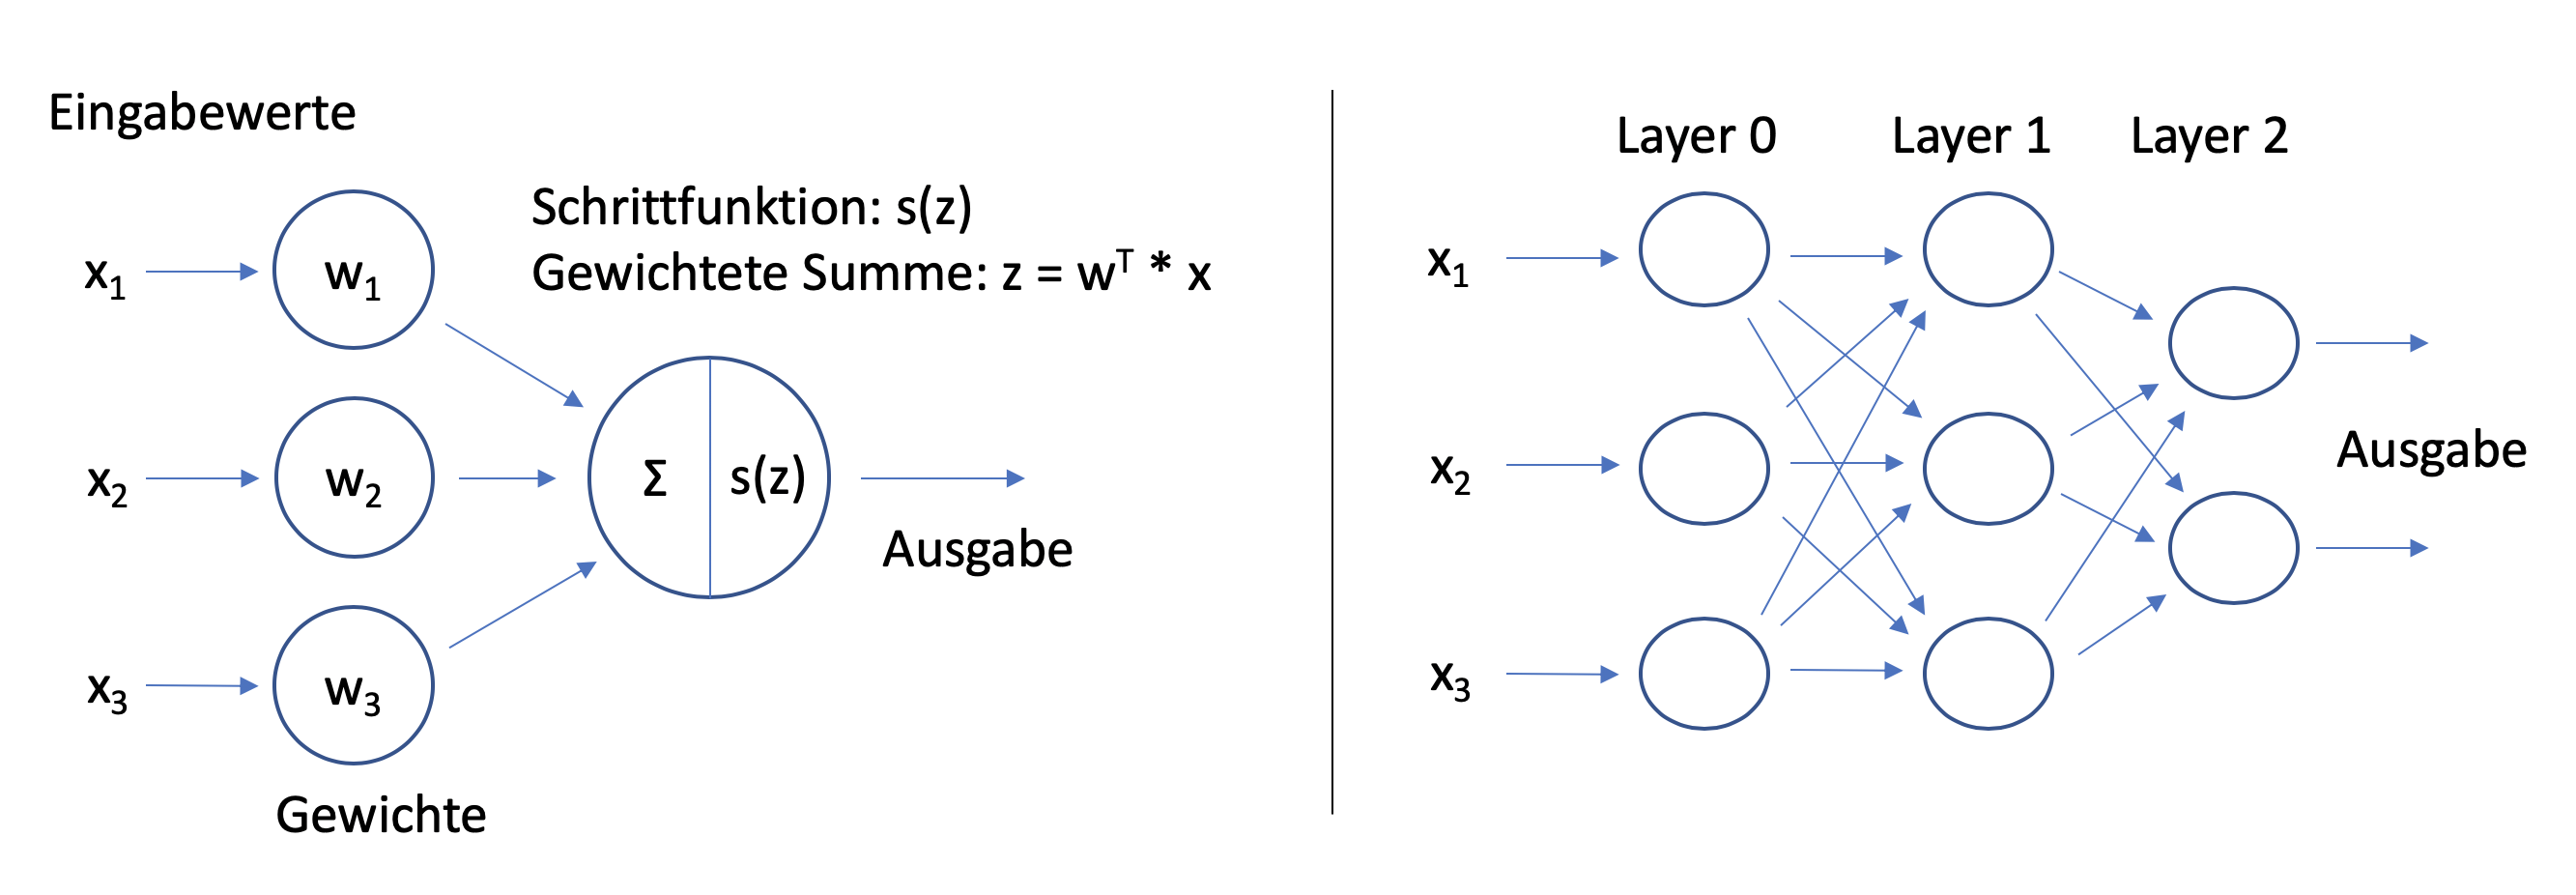
\includegraphics[width=\textwidth]{./images/perzeptron}
\label{fig_perzeptron}
\end{figure}

Für komplexere Aufgaben können Neuronen in mehreren Layern hintereinander geschalten werden (siehe Abbildung \ref{fig_perzeptron}). 
Die Neuronen in höheren Layern verwenden die Ausgabewerte des vorhergehenden Layers als Eingabewerte.
Die verwendete Modellstruktur sowie weitere Eigenschaften der einzelnen Neuronen (verwendete Schritt- / Aktivierungsfunktion, Anzahl Verbindungen zum vorherigen Layer) werden je nach der zu erledigenden Aufgabe gewählt \cite{francois_chollet_deep_nodate}.


\subsection{Bildklassifikation mit neuronalen Netzwerken}

Bei der Bildklassifikation sollen Bilder an Klassen zugeordnet werden. 
Für die Klassifikation mit neuronalen Netzwerken wird jeder Bildpunkt (bzw. Farbkanalwert) als Eingabewert für das Netzwerk verwendet. 
Das Netzwerk hat so viele Ausgabewerte, wie es auch Klassen erkennen soll. 
Jeder Ausgabewert wird einer Klasse zugeordnet. 
Dieser Ausgabewert entspricht der vom Netzwerk bestimmten Wahrscheinlichkeit, dass das Bild zu dieser Klasse gehört \cite{aurelien_geron_hands-machine_2017}. Dieser Ablauf ist in Abbildung \ref{fig_example_classifcation} visualisiert. Ein Bild einer Katze wird als Eingabewerte für den ersten Layer verwendet. Dessen Ausgabewerte wiederum gehen durch mehrere versteckte Layer. Die Ausgabe des letzten Layers entspricht den Wahrscheinlichkeiten pro Klasse, ob ein Objekt dieser Art im Bild vorhanden ist.

Zwischen Eingabe- und Ausgabe-Layer gibt es mehrere versteckte Layer. Analog des Multi-Layer-Perzeptrons verwenden sie jeweils die Ausgabe des vorhergehenden Layers als Eingabewerte. Die Neuronen in tieferen Layer (näher am Eingabe-Layer) sollen einfache Strukturen und Muster (z.B. Linien, Kanten) erlernen. Je höher der Layer liegt, umso komplexere Strukturen (z.B. Fell, Augen) werden von den Neuronen erlernt \cite{aurelien_geron_hands-machine_2017}.


\begin{figure}[h]
\caption{Eingabe- und Ausgabewerte eines neuronalen Netzwerkes für die Bildklassifikation}
\centering
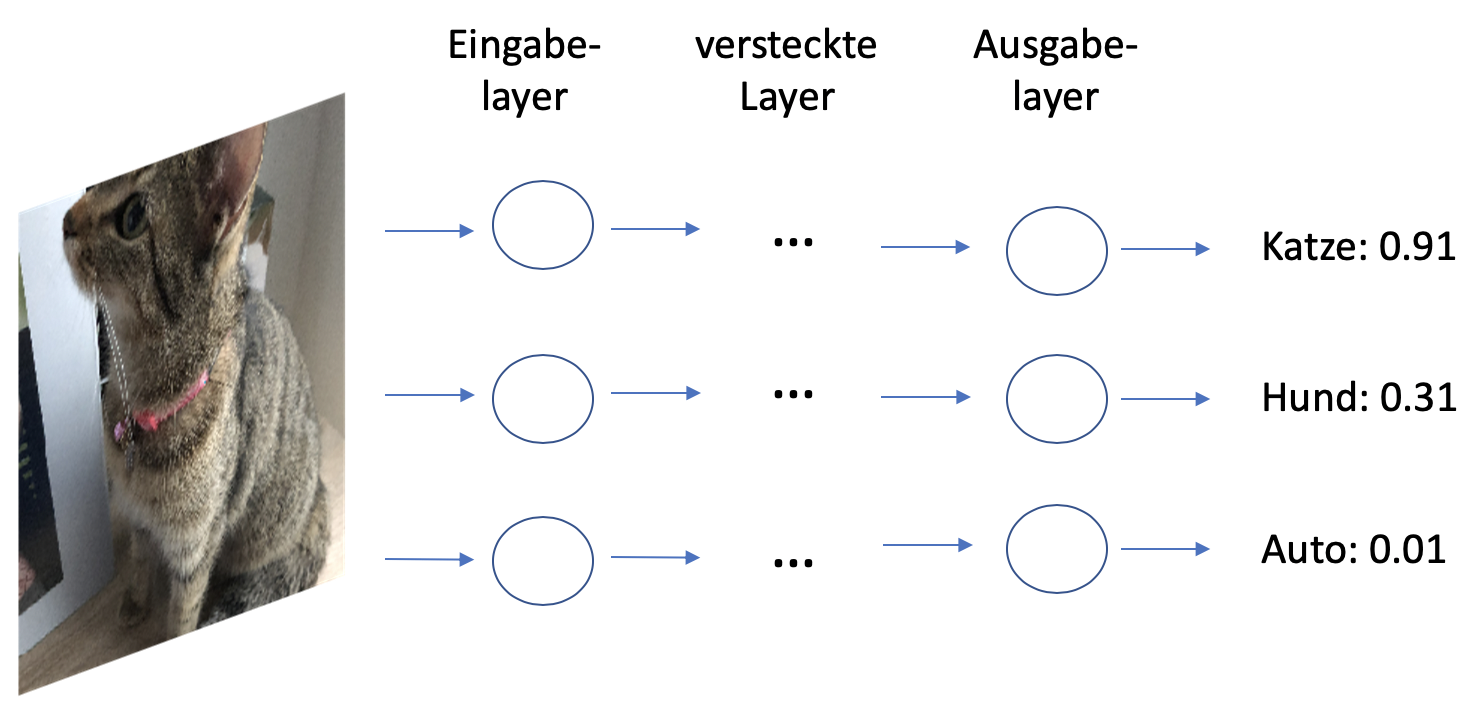
\includegraphics[width=0.8\textwidth]{./images/image_classification}
\label{fig_example_classifcation}
\end{figure}

In einem Multi-Layer-Perzeptron verwendet jedes Neuronen alle Ausgabewerte des vorherigen Layers zur Berechnung des eigenen Ausgabewertes. 
Das macht jedes einzelne Neuron sehr rechenaufwändig. Stattdessen werden in der Bilderkennung häufig Convolutional Layer verwendet.
Dabei handelt es sich um Layer, bei denen die einzelnen Neuronen nicht mehr jeden einzelnen Eingabewert des vorhergehenden Layers verwenden.
Stattdessen erhält jedes Neuron nur noch einen kleinen Bereich (z.B. ein $3 \times 3$-Bereich) aus dem vorhergehenden Layer (oder dem Eingabebild). Die Berechnung eines Neuron wird so bedeutend einfacher, da viel weniger Eingabewerte beachtet werden müssen \cite{aurelien_geron_hands-machine_2017}. Dadurch wird die nötige Rechenleistung während Anwendung und Training der Modelle verringert.


\section{Angriffe auf Bildklassifikatoren}

Angriffe auf Bildklassifikatoren haben zum Ziel, den angegriffenen Klassifikator zu täuschen. 
Der Klassifikator soll die wahre Klasse eines Bildes nicht mehr erkennen. 
Dafür wird das zu täuschende Bild verändert. 
In Abbildung \ref{fig_example_classifcation} wurde ein Modell visualisiert, das korrekt eine Katze erkennen kann. 
Die Klasse "Katze"{} hat die höchste Wahrscheinlichkeit aller möglicher Klassen. Durch eine Veränderung am Bild soll eine andere Klasse mit höchster Wahrscheinlichkeit erkannt werden.

Die Veränderung (der Störwert) soll üblicherweise so klein und unscheinbar wie möglich sein, damit sie sowohl maschinell als auch von Auge nicht erkannt werden kann. Sehr grosse Veränderungen am Bild werden von Auge sichtbar. Zudem könnte mit einer beliebigen Veränderung des Bildes auch die wahre Klasse des Bildes geändert werden (z.B. Bild der Katze durch ein Bild eines Autos ersetzen). 
Abbildung \ref{fig_example_misclassifcation} zeigt einen möglichen Störwert für das Katzenbild. 
Die Störungen im Bild sind klein genug, dass das Bild weiterhin für Menschen klar als Katze erkannt wird. 

\begin{figure}[h]
\caption{Beispiel eines Störwertes, das beim Inception-Modell beim Bild einer Katze eine Falschklassifikation verursacht. Unter dem Bild ist die Klasse angegeben, die Inception im Bild erkennt.}
\centering
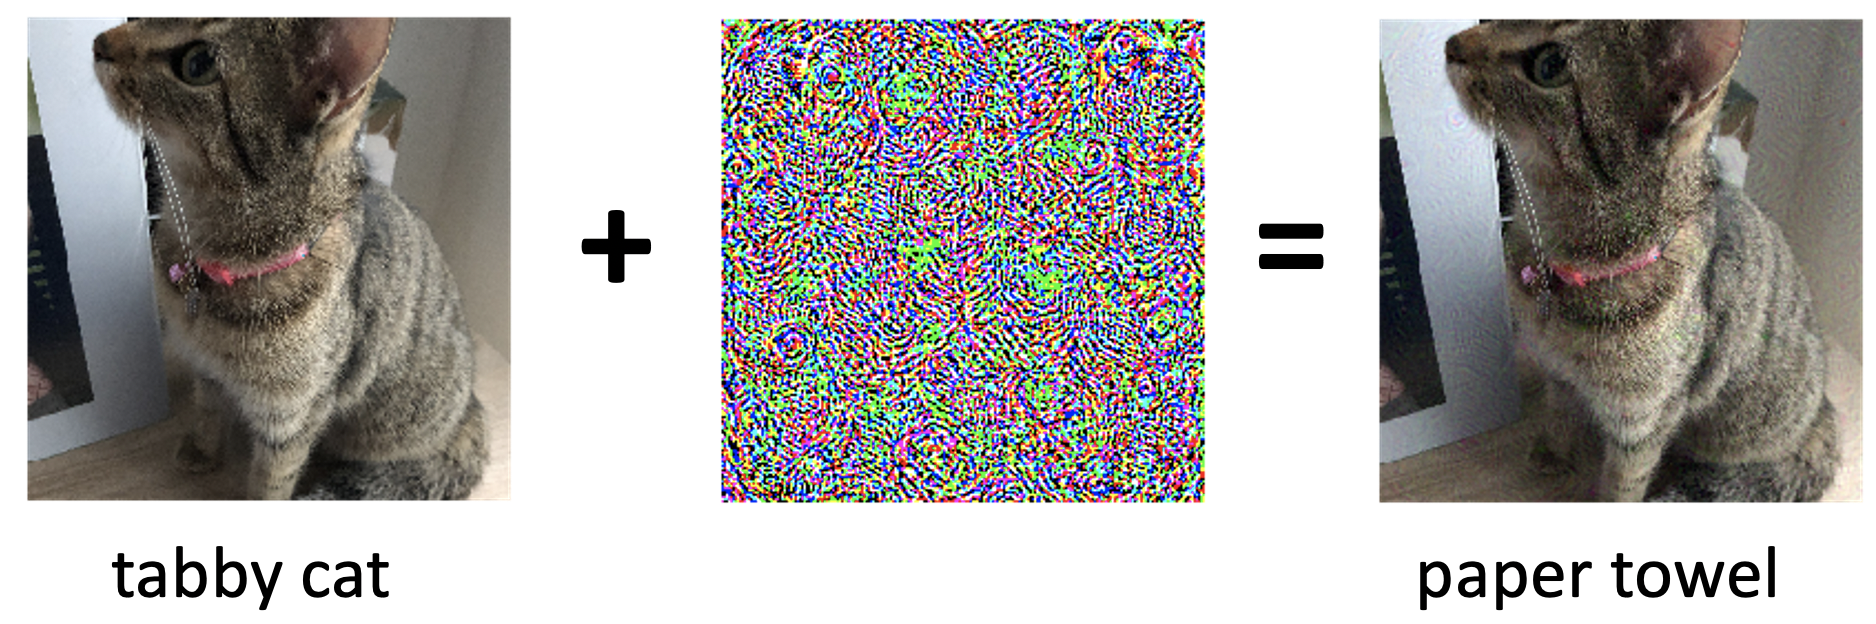
\includegraphics[width=0.8\textwidth]{./images/beispiel_falschklassifikation.png}
\label{fig_example_misclassifcation}
\end{figure}

\pagebreak

\subsection{Whitebox- und Blackbox-Angriffe}

Um den Störwert zu finden, braucht es Informationen über das anzugreifende Modell.
Je nach vorhandenen Informationen über das Modell wird zwischen zwei Arten unterschieden.
In einem Whitebox-Angriffsszenario kennt der Angreifer das anzugreifende System oder hat kompletten Zugriff auf das System. 
Für Bildklassifikatoren beinhaltet dies die verwendeten Modellstrukturen, Gewichte, verwendeten Trainingsdaten usw. 
Dieser direkte Zugang zum Modell erleichtert die Erstellung von Störwerten. 
Jede Veränderung am Bild kann überprüft werden, ob sie zum gewünschten Ziel hinführt. 
Der Angreifer sieht, wie sich die Wahrscheinlichkeiten der Klassen verändern. 

In einem Blackbox-Szenario sind diese Informationen nicht vorhanden \cite{sarkar_upset_2017}. 
Der Angreifer kennt das System nicht. 
Er erhält als einziges Feedback die Information, ob der Angriff erfolgreich war.
Er weiss nicht, ob eine Veränderung am Bild ihn näher ans Ziel führt oder nicht (wie die Störung die Wahrscheinlichkeiten veränderte). 

\subsection{Gezielte und ungezielte Störwerte}

Bei einem Angriff ist grundsätzlich das Ziel, dass das angegriffene Modell den Bildinhalt nicht mehr erkennt. Bei einem ungezielten Störwert wird nicht darauf geachtet, welche Klasse nach der Störung erkannt werden soll. Nach der Störung wird eine beliebige Klasse erkannt (ausser der wahren Klasse des Bildes).

Bei gezielten Angriffen soll durch die Störung eine spezifische Klasse erkannt werden.
Der Störwert muss also nicht mehr nur eine beliebige Falschklassifikation erzeugen, sondern das Modell eine spezifische Klasse erkennen lassen \cite{yuan_adversarial_2019}.

\subsection{Universelle Störwerte}

Störwerte werden in universelle und bildspezifische Störwerte unterteilt. 
Ein bildspezifischer Störwert wurde für ein einzelnes Bild erstellt. 
D.h. er soll genau bei einem Bild eine Falschklassifikation auslösen \cite{moosavi-dezfooli_deepfool_2016}. 
Ob der Störwert auch auf anderen Bildern die Klassifikation verändert, wird nicht geprüft. Möchte man ein anderes Bild stören, muss für dieses ein neuer Störwert generiert werden.

Universelle Störwerte sind bildunabhängig. Das heisst, der gleiche Störwert führt bei unterschiedlichen Bildern zu einer Falschklassifikation. Es muss nicht mehr pro Bild ein neuer Störwert errechnet werden \cite{moosavi-dezfooli_universal_2017-1, sarkar_upset_2017}. 




\subsection{Transferierbarkeit auf andere Modelle}

In \cite{papernot_transferability_2016} zeigen Papernot et al., dass Störwerte zum Angriff von Klassifikatoren zwischen Modellen übertragbar sind. Das heisst, ein Störwert, der für die Störung von Modell $A$ erstellt wurde, kann auch auf einem Modell $B$ eine Falschklassifikation verursachen.



Die Störwerte sind zu einem gewissen Grad unabhängig davon, mit welchen Daten der Klassifikator trainiert wurde. 
Die Störwerte sind auch auf andere Modellarchitekturen und Machine Learning-Verfahren übertragbar. Moosavi-Dezfooli et al. zeigen in \cite{moosavi-dezfooli_universal_2017-1}, dass auch grosse Modellstrukturen von transferierten Störwerten betroffen sind.

Baluja und Fischer zeigen in \cite{baluja_adversarial_2017}, wie mit einem ATN (Adversarial Transormation Network) Störwerte generiert werden können. Sie zeigen darin, dass das ATN durch Training auf mehreren Modellen Störwerte generiert, die auf allen zum Training verwendeten Modellen hohe Störraten erzielt.


\section{Definition einer Störung}

Wann ein Störwert ein Bild stört, ist je nach Literatur anders definiert. 
Die mit Störwert erkannte Klasse $\hat{y}$ wird entweder mit der wahren Klasse $y$ des Bildes oder der ohne Störwert erkannten Klasse $y_k$ verglichen \cite{moosavi-dezfooli_deepfool_2016, wiyatno_adversarial_2019}. 
Die wahre Klasse entspricht der Klasse, die tatsächlich dem Bildinhalt entspricht.

Der Unterschied entsteht durch die Bilder, bei denen der Klassifikator bereits ohne Störwert eine falsche Klasse erkennt. 
Wiyatno et al. argumentieren in \cite{wiyatno_adversarial_2019}, dass diese Bilder nicht für die Generierung von Störwerten verwendet werden sollten. 
Dies aus den Gründen, dass der Klassifikator bereits die falsche Klasse erkennt und eine Modifikation des Eingabebildes ungewollt zur korrekten Klassifikation führen kann.

In dieser Thesis gilt ein Bild erst dann als gestört, wenn $\hat{y} \neq y_k$ (die vom Modell erkannte Klasse muss ändern, unabhängig von der wahren Klasse des Bildes). 
Diese Definition wurde gewählt, damit die gemessenen Störraten mit denen von Moosavi-Dezfooli et al. verglichen werden können. Die Störrate $s$ gibt den Prozentsatz der Bilder in einem Datenset an, dessen Klassifikation durch den Angriff gestört werden konnten:

\[
s = \frac{\textnormal{Anzahl erfolgreich gestörter Bilder}}
			{\textnormal{Anzahl Bilder}} 
\]

\chapter{Universal Adversarial Perturbations}
\label{c_uap}

Die Störwerte werden mit dem Verfahren von Moosavi-Dezfooli et al. aus \cite{moosavi-dezfooli_universal_2017-1} erstellt. 
Das Verfahren generiert in einem Whitebox-Szenario ungezielte, universelle Störwerte.
Die anzugreifenden Modelle sind also für die Generierung der Störwerte bekannt. Da der Störwert universell ist, kann er auf beliebigen Bildern zu einer Falschklassifikation führen. Durch die Störwerte wird eine beliebige Klasse erkannt, es muss keine spezifische Klasse erkannt werden.


\begin{algorithm}
\caption{Berechnen universeller Störwerte, Universal Adversarial Perturbations \cite{moosavi-dezfooli_universal_2017-1}}
\label{alg_univ_stoerwert}
\begin{algorithmic}[1]

\State $X \gets$ Bilder-Trainingsset
\State $\hat{k} \gets$ Klassifikator
\State $\xi \gets l_p$-Norm des Störwertes
\State $\delta \gets$ max. Genauigkeit
\State \textbf{output}: universeller Störwert $\bold{v}$

\State $\bold{v} \gets 0$

\While {$ Err(X_v) \leq 1 - \delta $}

\For { $x_i \in X$ }

\If { $\hat{k}(\bold{x}_i + \bold{v}) = \hat{k}(\bold{x}_i) $}

\State Berechne minimalen Störwert für $\bold{x}_i + \bold{v}$

\State $\displaystyle \Delta \bold{v}_i \gets \arg \min_{r} \Vert \bold{r} \Vert_2$ s.d. $\hat{k}(\bold{x}_i + \bold{v} + \bold{r}) \neq \hat{k}(\bold{x}_i) $

\State aktualisiere den Störwert: \

\State $\bold{v} \gets \mathcal{P}_{p,\xi}(\bold{v} + \Delta \bold{v}_i)$

\EndIf
\State \textbf{end if}

\EndFor
\State \textbf{end for}

\EndWhile
\State \textbf{end while}

\end{algorithmic}
\end{algorithm}



\section{Verfahren}

Der Störwert $\bold{v}$ wird iterativ für einen Klassifikator $f$ auf einem Datensatz $X$ erstellt. 
In jeder UAP-Iteration (Universal Adversarial Perturbations) wird für jedes Bild $\bold{x}_i$ aus dem Datensatz geprüft, ob $\bold{v}$ eine Falschklassifikation auslöst. 
Dafür wird die Klasse des Originalbildes $\hat k(\bold{x}_i)$ mit der des gestörten Bildes verglichen $\hat k(\bold{x}_i + \bold{v}_i)$.

Löst $\bold{v}$ eine Falschklassifikation aus, wird der Störwert nicht verändert und zum nächsten Bild gewechselt. 
Führt das gestörte Bild noch nicht zur Falschklassifikation, wird für dieses einzelne Bild ein neuer Störwert errechnet. 
Es wird der minimale Störwert $\Delta \bold{v}_i$ gesucht, der für $\bold{x}_i + \bold{v}$ die Falschklassifikation auslöst. 
Das Berechnen minimaler Störwerte ist nicht Teil dieses Verfahrens, sondern geschieht mit DeepFool (siehe Kapitel \ref{c_deepfool}). 

Der minimale Störwert für das Bild wird zum Störwert $\bold{x}$ addiert. 
Die Norm dieses Störwerts wird begrenzt, damit dieser nicht zu gross (und damit sichtbar) wird.
Dies wird durch eine Funktion $\mathcal{P}_{p,\xi}(\bold{v})$ erreicht. Diese begrenzt den neuen Störwert auf die $l_p$-Norm mit Betrag $\xi$ . Dafür wird das $\bold{v'}$ mit kleinster Distanz zu $\bold{v}$ gesucht, das zusätzlich in der definierten $l_p$-Norm den Betrag $\xi$ nicht überschreitet \cite{moosavi-dezfooli_universal_2017-1}:

\[
\mathcal{P}_{p,\xi}(\bold{v}) = \arg \min_{\bold{v'}} \Vert \bold{v} - \bold{v'} \Vert_2
\textnormal{ unter der Bedingung } \Vert \bold{v'} \Vert_p \leq \xi
\]


\section{Begrenzen der Störwert-Norm}
\label{c_begrenzen_stoerwert_norm}

Grosse Störwerte hinterlassen auf den gestörten Bildern sichtbare Artefakte. 
Um das zu verhindern, wird die Norm der Störwerte begrenzt. 
Moosavi-Dezfooli et al. verwendeten in ihrer Arbeit die $l_2$- und $l_\infty$-Normen. 
Dabei handelt es sich um unterschiedliche $l_p$-Normen. Eine $l_p$-Norm auf einem Raum $\mathbb{K}^n$ ist definiert als \cite{kaballo_grundkurs_2018}: 

\[
\Vert \bold{x} \Vert_p = \Biggl(\sum_{j=1}^n \vert \bold{x}_j \vert^p \Biggl)^{1/p}, \bold{x} = (\bold{x}_1, \dots, \bold{x}_n) \in \mathbb{K}^n
\]


Für $p=\infty$ entspricht das dem maximalen Betrag über alle Komponenten in $\bold{x}$ \cite{kaballo_grundkurs_2018}:
\[
\Vert \bold{x} \Vert_\infty = \max_{j=1}^n \vert \bold{x}_j \vert, \bold{x} = (\bold{x}_1, \dots, \bold{x}_n) \in \mathbb{K}^n
\]

Die Wahl der Norm beeinflusst den generierten Störwert. 
Durch die $l_\infty$-Norm wird die maximale Veränderung pro Pixel- bzw. Farbkanal-Wert begrenzt, nicht aber des gesamten Störwertes. 
D.h. ein einzelner Farbkanal-Wert darf sich durch den Störwert maximal um $\xi$ verändern. 
Um den Störwert in der Norm zu halten, wird für jeden Farbkanal-Wert der kleinere Wert zwischen $\vert \bold{v} \vert$ und $\xi$ gewählt. 
Die Vorzeichen der Komponenten werden von $\bold{v}$ übernommen. 

\[
\mathcal{P}_{\infty,\xi}(\bold{v}) = sign(\bold{v}) \cdot \min(|\bold{v}|, \xi)) 
\]

Ist der Störwert ausserhalb der Norm, werden so nur die Farbkanal-Werte begrenzt, die auch ausserhalb von $\xi$ liegen. Alle anderen Farbkanal-Werte bleiben unverändert.
Mit $p=2$ (d.h. $l_2$-Norm) ergibt sich die euklidische Norm \cite{kaballo_grundkurs_2018}:

\[
\Vert \bold{x} \Vert_2 = \sqrt{\sum_{j=1}^n \vert \bold{x}_j \vert^2 }, \bold{x} = (\bold{x}_1, \dots, \bold{x}_n) \in \mathbb{K}^n
\]

 Im Falle der $l_2$-Norm werden nicht einzelne Farbkanal-Werte, sondern der gesamte Störwert begrenzt.
Bei einzelnen Farbkanal-Werten kann so eine grössere Veränderung geschehen, sofern entsprechend bei anderen Farbkanal-Werten kleinere Änderungen vorgenommen werden.
\[
\mathcal{P}_{2,\xi}(\bold{v}) = \bold{v} \cdot \min\Biggl(1, \frac{\xi}{ \Vert \bold{v} \Vert}\Biggl) 
\]

Ist der Störwert grösser $\xi$ (wenn $\frac{\xi}{ \Vert \bold{v} \Vert} > 1$), wird der Störwert mit $\frac{\xi}{ \Vert \bold{v} \Vert}$ multipliziert. Der Störwert entspricht so wieder der Grösse $\xi$. Durch die Normierung des Störwertes werden alle Farbkanal-Werte verändert. Beide Varianten zur Begrenzen der Störwert-Norm wurden aus dem zu \cite{moosavi-dezfooli_universal_2017-1} veröffentlichten Originalcode entnommen.

\section{Stoppkriterien}

Das Verfahren zur Berechnung der Störwerte ist abgeschlossen, sobald eine Mindeststörrate $s$ erreicht wurde. Die Störrate gibt den Prozentsatz der Bilder an, die durch den Angriff falsch klassifiziert wurden.
Definiert wird diese durch $\delta$, welches dem maximalen Prozentsatz korrekt erkannter Bilder entspricht: $s = 1 - \delta $.

Statt einer Mindeststörrate kann das Verfahren auch nach einer beliebigen Anzahl Iterationen $i_{max}$ abgebrochen werden. 
Dafür wird die in Algorithmus \ref{alg_univ_stoerwert} angegebene Abbruchbedingung durch $i \leq i_{max}$ ersetzt, wobei $i$ mit $0$ initialisiert und nach jeder Iteration um $1$ erhöht wird.

In \cite{moosavi-dezfooli_universal_2017-1} wurden keine Angaben gemacht, wie viele Iterationen durchlaufen wurden. 
Bei Tests mit dem Inception-Modell wurde nach zwei bis drei Iterationen eine Störrate von über $80\%$ erreicht (siehe Abschnitt \ref{c_resultate_reprod}). 
Es wird deshalb davon ausgegangen, dass nur wenige Iterationen notwendig sind. 
Bei allen Testläufen in dieser Arbeit wird nach spätestens $20$ Iterationen abgebrochen. 
Aufgrund der langen Laufzeiten des Verfahrens werden keine Tests mit mehr Iterationen durchgeführt.

\chapter{DeepFool}
\label{c_deepfool}

Zur Generierung des minimalen Störwertes $v_i$ in UAP wird DeepFool \cite{moosavi-dezfooli_deepfool_2016} verwendet. 
DeepFool ist ein iteratives Verfahren, das einen bildspezifischen Störwert für ein einzelnes Bild berechnet. Der generierte Störwert ist ungezielt. D.h. es wird nicht spezifiziert, welche Klasse durch die Störung erkannt werden soll. Das Modell wird eine beliebige andere Klasse erkennen.

\section{Verfahren}

DeepFool sucht die kleinste Veränderung des Eingabebildes, das zur Falschklassifikation führt. 
In Algorithmus \ref{alg_deepfool} ist der Ablauf des Verfahrens abgebildet. 
DeepFool benötigt zur Berechnung das zu störende Bild $x$ und den anzugreifenden Klassifikator $f$. 
DeepFool ist erfolgreich abgeschlossen, sobald die vom Klassifikator erkannte Klasse des modifizierten Bildes $\hat{k}(\bold{x}_i)$ nicht mehr der Klasse des Ursprungsbildes $\hat{k}(\bold{x}_0)$ entspricht.

In jeder Iteration wird für jede Klasse $k$ die Distanz vom Punkt $\bold{x}_i$ zur Klassengrenze $\hat{l}_k$ gesucht. 
Die Klassengrenze entspricht der Grenze, ab der die Klassifikation von einer Klasse zu einer anderen wechselt. 
Dafür wird für jede Klasse $k$ (ausser der ursprünglichen Klasse $\hat{k}(\bold{x}_0)$) die Gradientendifferenz $\bold{w'_k}$ und die Differenz der Ausgabewerte $f'_k$ zur Ursprungsklasse berechnet.

$\vert f'_k \vert$ entspricht der absolut benötigten Änderung des Ausgabewertes. 
$\Vert \bold{w'_k} \Vert_2$ ist die Richtung, in die der Eingabewert verändert werden kann, um die Ausgabewerte weg von der Klasse $\hat{k}(\bold{x}_0)$ hin zur Klasse $k$ verschoben wird. 
Aus diese beiden Werten ergibt sich die insgesamt notwendige Veränderung des Eingabebildes, um die Klassengrenze zu erreichen: $ \frac{ \vert f'_k \vert}{\Vert \bold{w'_k} \Vert_2}$.

Über alle Klassen wird nun die Klassengrenze $\hat{l}$ gewählt, für welche die kleinste Veränderung am Eingabebild notwendig ist. 
Die für diese Klassengrenze notwendige Veränderung $r_i$ wird zum modifizierten Bild $\bold{x}_i$ addiert.

Am Ende des Verfahrens enthält $\bold{x}_i$ das modifizierte Eingabebild (das eine Falschklassifikation auslöst). 
Die Summe von $\bold{x}_i$ über alle Iterationen entspricht dem Störwert, der das Bild an die Klassengrenze bringt. 
Gem. Moosavi-Dezfooli et al. erreicht DeepFool in einigen Fällen die Klassengrenze, geht aber nicht darüber hinaus \cite{moosavi-dezfooli_deepfool_2016}. 
Der Störwert wird deshalb mit $1+\eta$ ($\eta \ll 1$) multipliziert. 
So wird sichergestellt, dass die Klassengrenze übertreten, statt nur angenähert wird, da der Störwert so noch weiter in Richtung der Klassengrenze zeigt.

\begin{algorithm}
\caption{DeepFool für Mutliklassen-Klassifikatoren \cite{moosavi-dezfooli_deepfool_2016}, erweitert um $i_d$ und $\eta$}
\label{alg_deepfool}
\begin{algorithmic}[1]

\State $\bold{x} \gets$ Bild
\State $f \gets$ Klassifikator
\State $i_d \gets$ max. Iterationen
\State \textbf{output}: Störwert $\hat{\bold{x}}$

\State $\bold{x_0} \gets x$
\State $i \gets 0$

\While {$\hat{k}(\bold{x_i}) = \hat{k}(\bold{x_0}) $ \textbf{and} $ i \leq i_d$}

\For { $k \neq \hat{k}(\bold{x_0})$ }

\State $\bold{w'_k} \gets \nabla f_k(\bold{x_i}) - \nabla f_{\hat{k}(\bold{x_0})}(\bold{x_i}) $

\State $f'_k \gets f_k(\bold{x_i}) - f_{\hat{k}(\bold{x_0})}(\bold{x_i}) $

\EndFor
\State \textbf{end for}

\State $\hat{l} \gets \arg \min_{k \neq \hat{k}(\bold{x_0})} \frac{ \vert f'_k \vert}{\Vert \bold{w'_k} \Vert_2}  $

\State $\bold{r_i} \gets {\frac{\vert f'_{\hat{l}} \vert}{\Vert \bold{w'_{\hat{l}}} \Vert^2_2}} \bold{w'_{\hat{l}}} $

\State $\bold{x_{i+1}} \gets \bold{x_i} + \bold{r_i}$

\State $i \gets i + 1$

\EndWhile
\State \textbf{end while}

\State \textbf{return}: $\bold{\hat{r}} = (1 + \eta) \cdot \Sigma_i \bold{r_i} $

\end{algorithmic}
\end{algorithm}


\section{Stoppkriterien}

DeepFool stoppt, sobald eine Falschklassifikation des Eingabebildes erreicht wurde. 

In \cite{moosavi-dezfooli_deepfool_2016} wird angegeben, dass DeepFool oft nach drei bis vier Iterationen einen minimalen Störwert gefunden hat. 
Bei einigen Bildern kann DeepFool aber auch nach mehreren Iterationen noch keine Falschklassifikation erzeugen, deshalb wird die maximale Anzahl Iterationen mit $i_d$ beschränkt. 
Wurde nach $i_d$ DeepFool-Iterationen noch kein minimaler Störwert gefunden, wird das Verfahren abgebrochen. 
In diesem Fall war das Verfahren nicht erfolgreich und es wurde kein Störwert gefunden. In \cite{moosavi-dezfooli_universal_2017-1} und \cite{moosavi-dezfooli_deepfool_2016} wird dieses Abbruchkriterium nicht erwähnt, im veröffentlichten Beispielcode wurde mit $i_d = 10$ gearbeitet.

\section{Anzahl getesteter Klassen}

Auf die Anzahl getesteter Klassen wird in \cite{moosavi-dezfooli_deepfool_2016} nicht eingegangen.
In der Implementation werden aber nicht alle Klassen getestet, um die jeweils nächste Klassengrenze zu finden (Zeilen $8$ bis $11$ in Algorithmus \ref{alg_deepfool}). Stattdessen wird nur ein kleiner Teil der Klassen getestet. Es werden die Klassen mit den höchsten erkannten Wahrscheinlichkeiten geprüft. Diese Einschränkung dient als Performance-Optimierung des Verfahrens. So müssen nur noch für eine kleinere Anzahl Klassen die Gradienten berechnet werden. Zeit- und Speicherbedarf des Verfahrens nehmen so stark ab. Es ist dadurch möglich, dass nicht mehr die nächste Klassengrenze zum Bild gefunden wird. Der Störwert ist deshalb nicht zwingend der minimale Störwert, der zur Falschklassifikation führt.

\chapter{Optimieren der Transferierbarkeit}
\label{c_optimieren_transfer}

Nach Moosavi-Dezfooli et al. sind die von UAP errechneten Störwerte bereits teilweise auf andere Modelle transferierbar.
Dass die Störwerte transferierbar sind, lässt vermuten, dass es Störwerte gibt, die für mehr als nur ein Modell eine hohe Störrate erreichen. 
Die Störraten auf anderen Modellen sind bedeutend geringer als auf dem Modell, für das die Störwerte generiert wurden (siehe Abschnitt \ref{c_resultate_transferierbarkeit}). 
Um eine hohe Störrate auf zwei Modellen zu erhalten, werden beide Modelle in die Generierung des Störwerts mit einbezogen. 
Es werden vier Kombinationsverfahren getestet, welche das zweite Modell in zunehmenden Masse in die Generierung des Störwertes einbeziehen. 
Durch zunehmende Integration in die Generierung der Störwerte sollte ein immer besserer Störwert für beide Modelle entstehen. 
Da der so generierte Störwert für zwei Modelle hohe Störraten erreicht, sollte er auch auf einem dritten Modell höhere Störraten erzielen, das nicht für die Generierung verwendet wurde.

\section{Lineare Interpolation von Störwerten}

Für die erste Kombination werden mit UAP Störwerte für zwei Modelle $f$ und $g$ generiert. 
Diese Störwerte können als Punkte in einem hochdimensionalen Raum interpretiert werden. 
Sofern es einen Störwert gibt, der auf $f$ und $g$ hohe Störraten erzielt, sollten zwischen diese beiden Punkten andere Störwerte sein, die beide Modelle stören können. 
Um das zu prüfen, wird eine Gerade durch die beiden Punkte gelegt. 
Aus dieser Geraden werden Punkte zwischen den beiden Störwerten gewählt und als Störwerte verwendet.

Die Gerade $h$ ist in Parameterform definiert als \cite{rolf_socher_mathematik_2011}:

\[
h = \vec{OP} + \langle  PQ \rangle 
\]

$\vec{OP}$ ist der Stützpunkt der Geraden. 
Dieser Punkt definiert die Verschiebung der Geraden vom Ursprung (dem Nullvektor) weg. 
$\langle PQ \rangle $ ist ein Richtungsvektor, der die Richtung der Geraden angibt.

\pagebreak

Als Punkte $P$ und $Q$ werden nun die beiden Störwerte verwendet. 
D.h. die Gerade startet bei einem Störwert und zeigt in Richtung des anderen Störwertes. 
$\langle PQ \rangle $ kann durch $Q-P$ berechnet werden. 
Jedes Vielfache von $\langle PQ \rangle $ entspricht einem Punkt auf $h$ \cite{rolf_socher_mathematik_2011}. 
Die Punkte zwischen $P$ und $Q$ werden durch das Skalieren von $\langle PQ \rangle $ berechnet. 
Es werden $20$ gleichmässig verteilte Punkte zwischen den Punkten $P$ und $Q$ gewählt. 
Diese Punkte bilden die neuen Störwerte (in Abbildung \ref{fig_interpolation_example} orange abgebildet).

\begin{figure}[h]
\caption{Visualisierung der per linearer Interpolation generierten Störwerte in einem zweidimensionalen Raum}
\centering
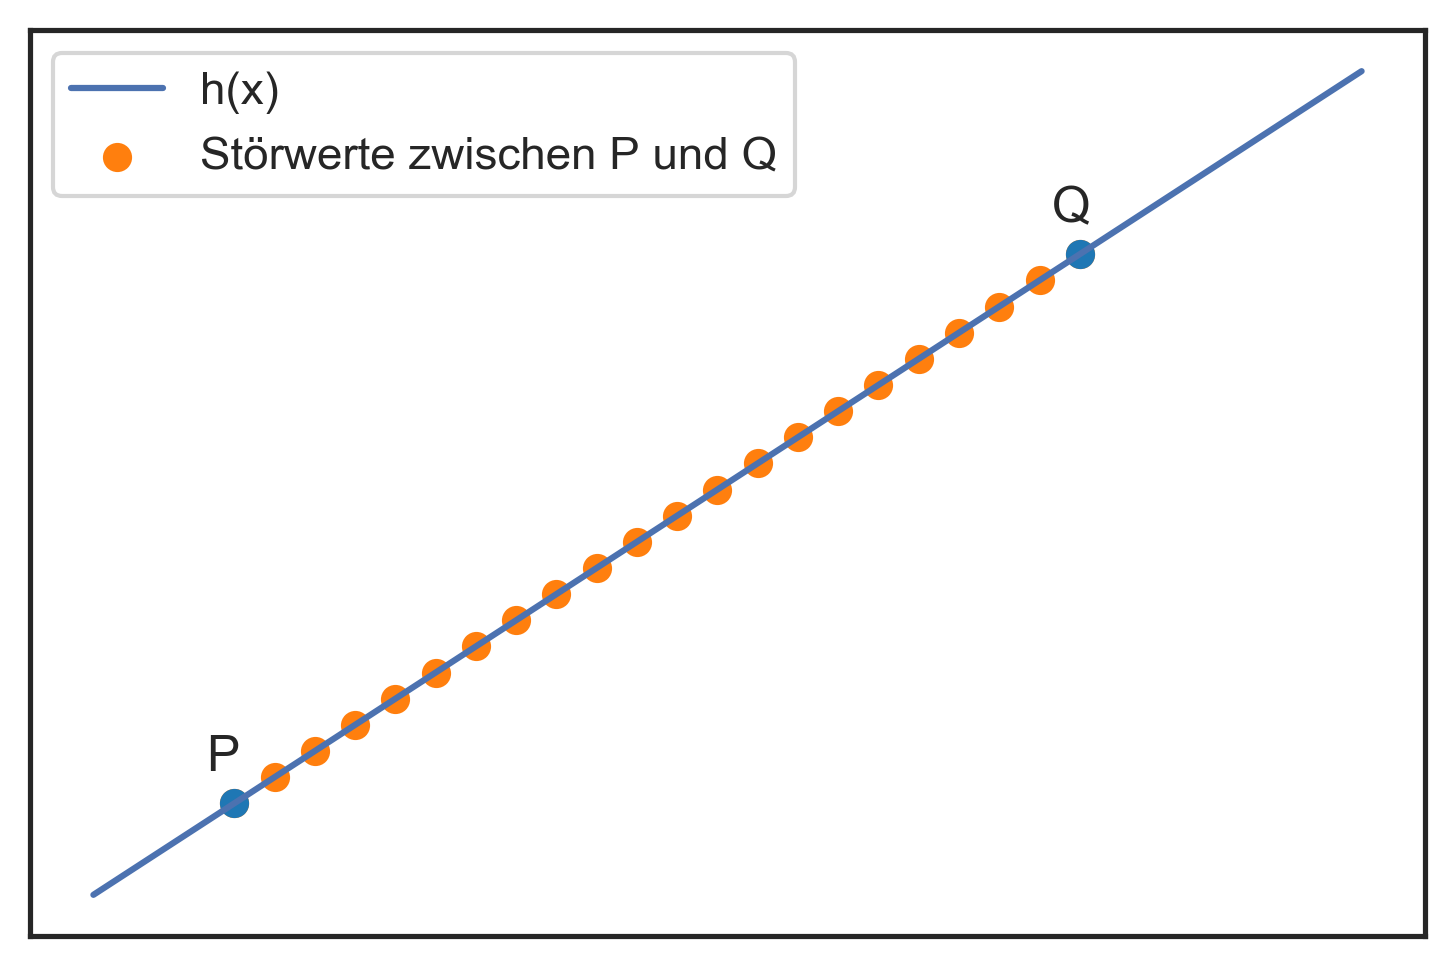
\includegraphics[width=0.6\textwidth]{./images/lin_interpol_example}
\label{fig_interpolation_example}
\end{figure}


\section{Finetuning eines bestehenden Störwertes}

Das Prinzip dieses Verfahrens basiert auf dem Transfer-Learning von Modellen \cite{shao_transfer_2015}. 
Damit werden bereits trainierte Modelle für andere Datensets wiederverwendet. 
Da es bereits trainiert wurde, kann es mit wenigen Trainingsdaten und Iterationen auf ein neues Datenset trainiert werden.

Analog wird dies auf die Generierung von Störwerten angewandt: Beim Finetuning des Störwertes wird als erstes für ein Modell $f$ ein Störwert $\bold{v}_f$ mit UAP generiert. 
Anschliessend wird UAP nochmals für ein zweites Modell $g$ durchgeführt. 
Für Modell $g$ wird $\bold{v}$ zu Beginn mit $\bold{v}_f$ statt mit $0$ initialisiert. 
Im UAP-Durchlauf für Modell $g$ wird so der Störwert $\bold{v}_f$ nur für die Bilder erweitert, bei denen der Störwert auf Modell $g$ keine Falschklassifikation auslöst. 
Dies ergibt sich aus Zeile $9$ in Algorithmus \ref{alg_univ_stoerwert}, bei erfolgreich gestörten Bildern wird $v$ nicht verändert. 

Der Störwert sollte sich durch das Finetuning nur minimal verändern. 
Dadurch sollte die Störrate auf Modell $f$ trotz des Finetunings hoch bleiben. 
Durch diese minimalen Veränderungen sollte sich auf Modell $g$ ebenfalls eine höhere Störrate ergeben als bei einem nur auf Modell $f$ berechneten Störwert.


\section{Abwechselndes Generieren auf zwei Modellen}

Statt den Störwert zuerst für Modell $f$ zu berechnen und dann in Richtung des Störwertes von $g$ zu verändern, kann bei der Generierung auch direkt in Richtung der beiden Störwerte gearbeitet werden.

UAP wird dahingehend erweitert, dass Störwerte für zwei Klassifikatoren auf einmal generiert werden. 
Dafür werden nachfolgende Änderungen am Algorithmus \ref{alg_univ_stoerwert} gemacht. 

Das Verfahren nimmt neu zwei Klassifikatoren, $f$ und $g$, entgegen. 
Als Abbruchbedingung für das Verfahren muss die Störrate neu auf beiden Klassifikatoren erreicht werden. 
Nach jedem Bild $\bold{x}_i$ wird der verwendete Klassifikator gewechselt. 
D.h. Zeilen $9$ - $11$ in Algorithmus \ref{alg_univ_stoerwert} werden abwechselnd für $f$ und $g$ ausgeführt.

Beim Generieren wird der Störwert so ständig entweder in Richtung des Störwertes für $f$ oder $g$ hin optimiert. 
Dadurch sollte der Störwert schlussendlich in eine Richtung zeigen (bzw. Wert enthalten), die beide Modelle optimal stört.


\section{DeepFool für mehrere Modelle}
\label{c_multifool}

Die bisher beschriebenen Verfahren verwenden DeepFool, um pro Bild im Datenset den Störwert für ein Modell zu errechnen. 
Das hat beim Training auf zwei Modellen einen Nachteil. 
Angenommen es gibt ein Bild, für das der Störwert für Modell $f$ in die entgegengesetzte Richtung wie der für Modell $g$ zeigt. 
Je nach Modell wird der Störwert nun in die eine oder andere Richtung optimiert. 
Es wird aber nie ein Störwert gefunden, der beide Modelle stören kann. 
Der mit UAP generierte Störwert lernt so nie, wie das Bild für beide Modelle gestört werden kann.

Statt die beiden Modelle nur abwechselnd für die Generierung zu verwenden, können auch einzelne Bilder direkt für beide Modelle gestört werden. 
DeepFool wird so erweitert, dass ein minimaler Störwert gefunden werden kann, der zwei Modelle stört. 
Das Stoppkriterium von DeepFool wird erweitert: Das Verfahren ist erst abgeschlossen, wenn bei beiden Klassifikatoren eine Falschklassifikation erzeugt wird (Zeile $8$ in Algorithmus \ref{alg_multifool}).



DeepFool suchte in jeder Iteration die nächste Klassengrenze $\hat{l}$ zu $\bold{v}_i$, dem teilweise gestörten Bild \cite{moosavi-dezfooli_deepfool_2016}. 
Nun wird für beide Modelle eine Klassengrenze gesucht. 
Es ist nicht mehr pro Modell die nächste Klassengrenze. 
Stattdessen wird das Klassengrenzen-Paar $\hat{l}_f$ und $\hat{l}_g$ gesucht, dass zusammen die minimale Veränderung am Eingabebild benötigt. 
Dafür wird für jedes Modell unabhängig vom anderen Modell die nächste Klassengrenze gesucht. 
Die Grenzen $\hat{l}_f$ und $\hat{l}_g$ können deshalb zu unterschiedlichen Klassen gehören. 

Nachdem die Klassengrenzen gefunden wurden, wird der Eingabewert in Richtung beider Klassengrenzen verändert. 
Als zu erreichende Veränderung im Ausgabewert wird die Summe beider Ausgabewert-Distanzen verwendet ($\vert f'_k \vert + \vert g'_k \vert$). 


\begin{figure}[h]
\caption{Kombination der beiden Störrichtungen pro Bild. Die beiden Distanzen zu den Klassengrenzen $l_g$ und $l_f$ (blaue Pfeile) werden addiert. Die resultierende Störung (grüner Pfeil) liegt für beide Klassifikatoren hinter der Klassengrenze.}
\centering
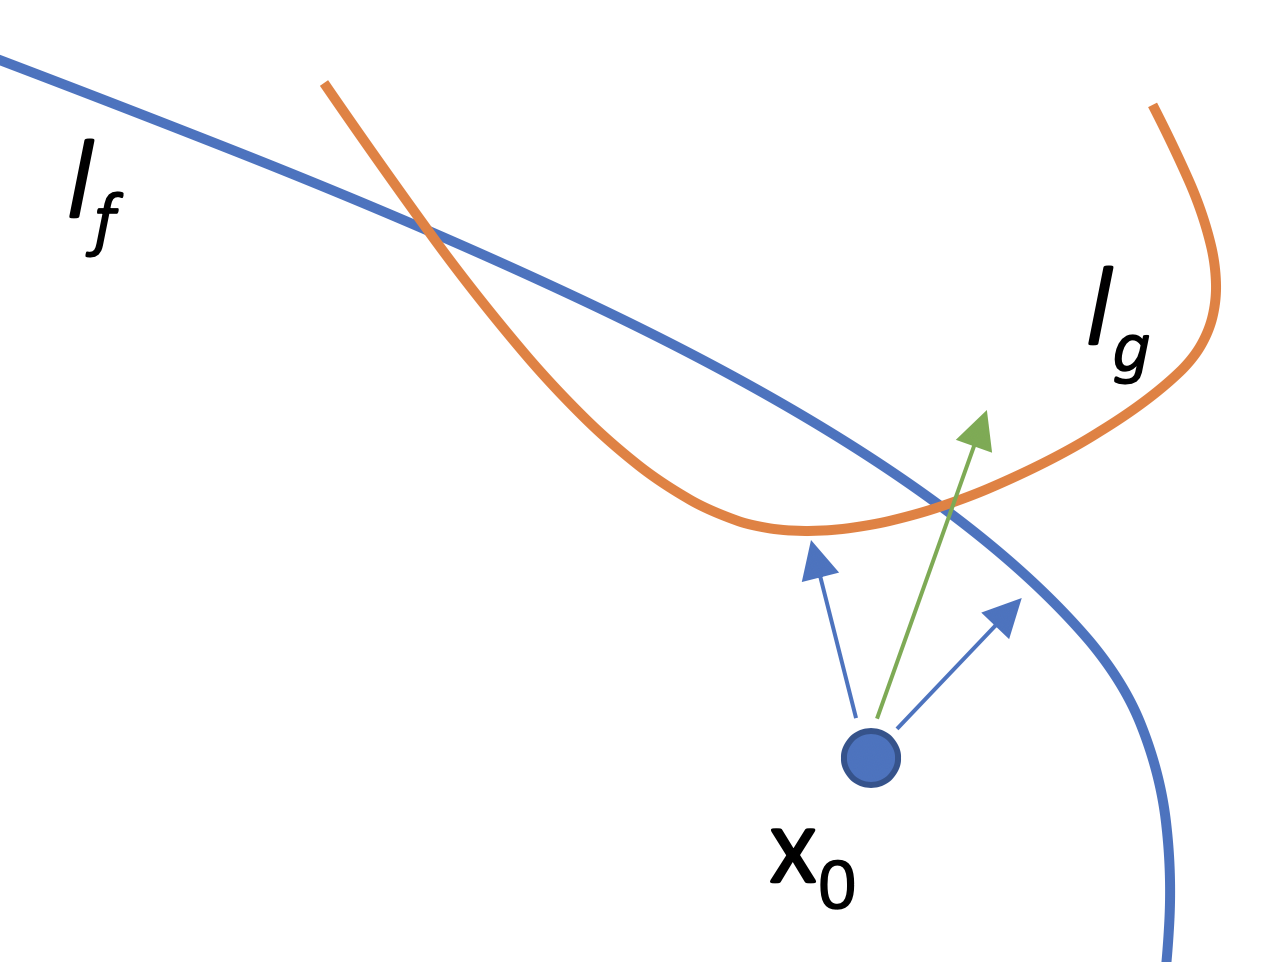
\includegraphics[width=0.5\textwidth]{./images/2d_multifool}
\label{fig_multifool}
\end{figure}

 Die Richtung ist die Summe der beiden einzelnen Richtungen $\bold{w'_k} + \bold{z'_k}$. In Abbildung \ref{fig_multifool} ist visualisiert, wie der Störwert so die Klassengrenze für zwei Modelle erreichen kann. Die darin dargestellten einzelnen Störwerte führen nicht direkt zur Falschklassifikation des anderen Klassifikators. Die Kombination der beiden führt wiederum in eine Richtung, die für beide Modelle eine Falschklassifikation auslöst.
 
 Andere Kombinationsvarianten der Distanzen wurden ebenfalls getestet (min-, max-, avg-Distanz). Für die Richtung wurden Tests mit der Winkelhalbierenden von $\bold{w'_k}$ und $\bold{z'_k}$ durchgeführt. Die Berechnung der Störwerte benötigte in diesen Konstellationen über $100$ DeepFool-Iterationen. Das unveränderte DeepFool-Verfahren benötigt nur $3$-$4$ Iterationen für die Berechnung \cite{moosavi-dezfooli_deepfool_2016}. Diese Kombinationsvarianten wurden deshalb nicht weiter verfolgt. Mit der Addition von Distanz und Richtung kann der Störwert nach ca. $20$ Iterationen erfolgreich beide Klassifikatoren stören.
 
 
\begin{algorithm}
\caption{DeepFool für zwei Klassifikatoren}
\label{alg_multifool}
\begin{algorithmic}[1]

\State $x \gets$ Bild
\State $f \gets$ Klassifikator $1$
\State $g \gets$ Klassifikator $2$
\State $i_d \gets$ max. Iterationen
\State \textbf{output}: Störwert $\hat{r}$

\State $x_0 \gets x$
\State $i \gets 0$

\While {$(\hat{k}_f(\bold{x_i}) = \hat{k}_f(\bold{x_0})$ \textbf{or} $\hat{k}_g(\bold{x_i}) = \hat{k}_g(\bold{x_0}))$ \textbf{and} $ i \leq i_d$}

\For { $k \neq \hat{k}_f(\bold{x_0})$ }

\State $\bold{w'_k} \gets \nabla f_k(\bold{x_i}) - \nabla f_{\hat{k}(\bold{x_0})}(\bold{x_i}) $

\State $f'_k \gets f_k(\bold{x_i}) - f_{\hat{k}(\bold{x_0})}(\bold{x_i}) $

\EndFor
\State \textbf{end for}

\For { $k \neq \hat{k}_g(\bold{x_0})$ }

\State $\bold{z'_k} \gets \nabla g_k(\bold{x_i}) - \nabla g_{\hat{k}(\bold{x_0})}(\bold{x_i}) $

\State $g'_k \gets g_k(\bold{x_i}) - g_{\hat{k}(\bold{x_0})}(\bold{x_i}) $

\EndFor
\State \textbf{end for}


\State $\hat{l}_f, \hat{l}_g \gets \arg \min_{k_f \neq \hat{k}_f(\bold{x_0}) \bold{and} k_g \neq \hat{k}_g(\bold{x_0})} \frac{ \vert f'_k \vert + \vert g'_k \vert}{\Vert \bold{w'_k} + \bold{z'_k} \Vert_2}  $



\State $\bold{r_i} \gets {\frac{ \vert f'_k \vert + \vert g'_k \vert }{\Vert \bold{w'_k} + \bold{z'_k} \Vert^2_2}} (\bold{w'_k} + \bold{z'_k}) $

\State $\bold{x_{i+1}} \gets \bold{x_i} + \bold{r_i}$

\State $i \gets i + 1$

\EndWhile
\State \textbf{end while}

\State \textbf{return}: $\bold{\hat{r}} = \Sigma_i \bold{r_i} $

\end{algorithmic}
\end{algorithm}




\chapter{Versuchsaufbau}
\label{c_versuchsaufbau}

Die Qualität der aus den Kombinationsverfahren erstellten Störwerte hängt davon ab, wie hohe Störraten die unveränderten UAP- und DeepFool-Verfahren liefern. Um diese Frage zu beantworten, werden die beiden Verfahren implementiert und getestet. Sie werden in der gleichen Konfiguration durchgeführt, wie in \cite{moosavi-dezfooli_universal_2017-1} beschrieben wurde, um deren Resultate möglichst exakt nachzustellen.

Um anschliessend die Qualität der mit den Kombinationsverfahren generierten Störwerte zu messen, werden diese ebenfalls implementiert und experimentell getestet. 

\section{Versuchsablauf}

Für verschiedene Modelle werden Störwerte gemäss dem Verfahren von Moosavi-Dezfooli et al. aus \cite{moosavi-dezfooli_universal_2017-1} generiert. 
Die Transferierbarkeit auf andere Modelle wird auf diesen Störwerten gemessen. 
Anschliessend werden einzelne Parameter der UAP- und DeepFool-Verfahren daraufhin überprüft, welchen Einfluss sie auf die Störrate der Modelle haben. Dafür wird jeweils ein Parameter gewählt und dessen Wert verändert. Bei den Tests wird immer nur ein Parameter geändert und getestet. Es werden keine Kombinationen von anderen Werten getestet.

Die in Kapitel \ref{c_optimieren_transfer} beschriebenen Kombinationsverfahren werden anschliessend mit einer Modellkombination getestet. Alle Verfahren werden mit der gleichen Modellkombination getestet, damit die Störraten miteinander vergleichbar bleiben.

Die Störrate wird für jeden generierten Störwert auf dem verwendeten Trainings- und dem Validation-Set gemessen. 
Zusätzlich wird die Störrate nach jeder UAP-Iteration für beide Sets berechnet (d.h. nach jedem Durchgang durch das Trainingsset).

\pagebreak

\section{Parameterwahl Reproduktion}
\label{c_parameterwahl}

Für die Reproduktion der Ergebnisse aus \cite{moosavi-dezfooli_universal_2017-1} wurden die darin beschriebenen Parameterkonfigurationen übernommen. 
Daraus wurden die Grösse des Trainingsset ($10'000$ Bilder) und die Störwert-Normen ($l_2$ mit $\xi=2'000$ und $l_\infty$ mit $\xi=10$) übernommen. 
Es wurde nicht dokumentiert, welches Stoppkriterium $\delta$ gewählt wurde. 
Das Stoppkriterium wird deshalb für die Replikation nicht verwendet. 
Stattdessen wird das Verfahren immer für eine fixe Anzahl an Iterationen ausgeführt (siehe Kapitel \ref{c_uap}). 
Aufgrund der langen Laufzeiten des UAP-Verfahrens werden alle Tests auf maximal $20$ Iterationen beschränkt.


Für die Wahl der DeepFool-Parameter ($\eta$, max. Anzahl DeepFool-Iterationen, Anzahl geprüfter DeepFool-Klassen) wurden in \cite{moosavi-dezfooli_universal_2017-1} keine Angaben gemacht. Die Autoren wurden diesbezüglich angeschrieben, bis zum Zeitpunkt der Abgabe dieser Arbeit wurde aber noch keine Antwort erhalten.

Für $\eta$ wurde deshalb der gleiche Wert gewählt, wie in der Arbeit zu DeepFool selbst erwähnt wurde ($0.02$) \cite{moosavi-dezfooli_deepfool_2016}. 
Die anderen beiden Parameter wurden aus dem zu \cite{moosavi-dezfooli_universal_2017-1} veröffentlichten Originalcode entnommen ($10$ für beide Parameter), da sie in der Arbeit zu DeepFool nicht erwähnt werden. 

Es ist nicht auszuschliessen, dass je nach Modell unterschiedliche Parameter für die Verfahren verwendet wurden. Die nicht dokumentierten Parameter werden deshalb einzeln daraufhin überprüft, wie sie die Störrate verändern. 

\section{Modellauswahl}
\label{c_modelle}


\begin{table}[]
\centering
\caption{Verwendete Testmodelle}
\begin{tabular}{|l|r|l|}
\hline
Modell				& Top-1 Erkennungsrate	& Referenz						\\ \hline
Inception			& $77.898\%$				&	\cite{szegedy_going_2015}	\\
ResNet-152			& $78.032\%$  			&	\cite{he_deep_2016}			\\
VGG-16				& $71.268\%$  			&	\cite{simonyan_very_2014}	\\
VGG-19				& $71.256\%$     		&	\cite{simonyan_very_2014}	\\
VGG-F				& $58.9\%$    			&	\cite{chatfield_return_2014}\\
\hline 
\end{tabular}
\label{tbl_verwendete_modelle}
\end{table}


Das Verfahren wird mit den in Tabelle \ref{tbl_verwendete_modelle} aufgelisteten Modellen getestet. Die darin angegebenen Top-1 Erkennungsraten wurden auf dem ImageNet Validation-Set gemessen.
Es werden die gleichen Modelle verwendet wie in \cite{moosavi-dezfooli_universal_2017-1}. 
Die in dieser Thesis erzielten Störraten können so mit denen der Originalarbeit verglichen werden. Aktuellere Modelle (wie z.B. DenseNet \cite{huang_densely_2017} oder EfficientNet \cite{tan_efficientnet_2019}) wurden nicht getestet, da deren Störraten nicht mit denen der Originalarbeit verglichen werden können.
Die gewählten Modelle beinhalten sowohl sehr ähnliche Modelle (VGG-16 und VGG-19), aber auch Modelle mit unterschiedlichen Modellstrukturen (z.B. Inception und ResNet-152).
Analog der Originalarbeit zu UAP \cite{moosavi-dezfooli_universal_2017-1} wird bei allen Modellen die Aktivierungsfunktion des Ausgabe-Layers entfernt. 

Von allen Modellen werden vortrainierte Varianten verwendet, es wurden keine Modelle selbst trainiert. 
Für ResNet-152, Inception, VGG-16 und VGG-19 wurden die auf ImageNet \cite{russakovsky_imagenet_2015} vortrainierten Gewichte von TensorFlow \cite{martin_abadi_tensorflow_2015} verwendet. 
Die Gewichte von VGG-F entsprechen den zu \cite{chatfield_return_2014} veröffentlichten Gewichten. 
Die VGG-F Gewichte wurden mit caffe-tensorflow\footnote[1]{Abrufbar unter https://github.com/ethereon/caffe-tensorflow} von Caffe \cite{jia_caffe:_2014} zu TensorFlow konvertiert.

\section{Messen der Störrate}
\label{c_messen_stoerrate}

Eine Klassifikation wird als erfolgreich gestört betrachtet, wenn die Klasse mit der höchsten Wahrscheinlichkeit gemäss Klassifikator ändert. 
Die Störrate $s$ auf einem Datensatz $X$ entspricht dem Prozentsatz aller Bilder, deren Klassifikation durch den Störwert verändert wurde.
Die tatsächliche Klasse des Bildes ist für die Bestimmung der Störrate irrelevant.


\section{Verwendete Materialien}

Die Implementationen von Deepfool und UAP basieren auf dem zur Originalarbeit veröffentlichten Code \cite{moosavi-dezfooli_universal_2017-1, moosavi-dezfooli_deepfool_2016}. Die ursprünglich verwendeten Bibliotheksversionen sind nicht bekannt. Der Code wurde nach TensorFlow $2.0.0$ migriert und verwendet u.a. auch die Bibliotheken aus Tabelle \ref{tbl_verwendeteBibliotheken}. Zusätzlich wurden Änderungen vorgenommen, um die Daten via Tensorflow Datasets zu laden und beliebige Modelle zu stören. Der Code für das UAP-Verfahren und die Kombinationsverfahren ist in den Zusatzmaterialien zu dieser Thesis vorhanden.

Alle Störwerte wurden in einer virtuellen Maschine mit vier Intel Skylake vCPUs, einer Nvidia Tesla K80 und 26 GB Arbeitsspeicher berechnet.

\begin{table}[]
\centering
\caption{Verwendete Bibliotheken}
\begin{tabular}{|l|l|}
\hline
Bibliothek          & Version   \\ \hline
Tensorflow          & $2.0.0$   \\
Tensorflow Datasets & $1.3.2$   \\
Numpy               & $1.17.4$  \\
Python              & $3.7$     \\
Nvidia CUDA         & $10.1$    \\
\hline 
\end{tabular}
\label{tbl_verwendeteBibliotheken}
\end{table}


\pagebreak

\section{Datensatz}

Für die Generierung und Validierung von Störwerten wird der ILSVRC2012 ImageNet-Datensatz \cite{russakovsky_imagenet_2015} verwendet. 
Der Datensatz wurde von TensorFlow in der Version $2.0.1$ bezogen \cite{martin_abadi_tensorflow_2015}. 
Der Datensatz beinhaltet ein Trainings-Set mit $1'200'000$ Bildern und ein Validation-Set mit $50'000$ Bildern. 
Jedes Bild ist einer von $1'000$ Klassen zugeordnet, die den Bildinhalt beschreibt. 
Die wahren Klassen sind zu allen Bildern in beiden Datensets enthalten. 

Für die Generierung von Störwerten wird analog zu \cite{moosavi-dezfooli_universal_2017-1} ein zufällig gewähltes Subset aus dem Trainings-Set mit $10'000$ Bildern verwendet. 
Sofern nicht anders erwähnt, wurde für alle Störwerte das gleiche Subset verwendet. 
Für die Validierung von Störwerten wird das komplette Validation-Set des ImageNet-Datensatzes verwendet. 

Die Bilder haben keine einheitliche Grösse. 
Damit die Bilder mit DNNs klassifiziert werden können, werden sie in einem Preprocessing-Schritt in eine einheitliche Grösse gebracht.


\subsection{Preprocessing}

Das Preprocessing der Bilder ist essentiell, um die in Abschnitt \ref{c_modelle} angegebenen Erkennungsraten zu erreichen. 
Bereits kleine Änderungen am Preprocessing können zu tieferen Erkennungsraten führen. 
Auf alle Bilder werden zwei Preprocessing-Schritte angewandt, bevor sie für die Generierung oder Validierung von Störwerten verwendet werden.
Die Bilder werden auf die Grösse $224 \times 224 \times 3$ (Breite, Höhe, Anz. Farbkanäle) transformiert. 
Dafür wird die kleinere der beiden Seiten, $w$ oder $h$, bikubisch auf $224$ Pixel skaliert. 
Die grössere Seite wird proportional mitskaliert. 
Von der zweiten, grösseren, Seite werden $224$ Pixel aus der Mitte ausgeschnitten. 
Das resultierende Bild hat die Grösse $224 \times 224 \times 3$. 
In Abbildung \ref{fig_preprocessing} sind die beiden Schritte anhand eines Bildes visualisiert. 
Dieses Skalierungs-Vorgehen entspricht dem in \cite{chatfield_return_2014} beschriebenen Test-Preprocessing. Es wird für die Tests aller Modelle in dieser Thesis verwendet. 


\begin{figure}[h]
\caption{Center-Crop eines Bildes}
\centering
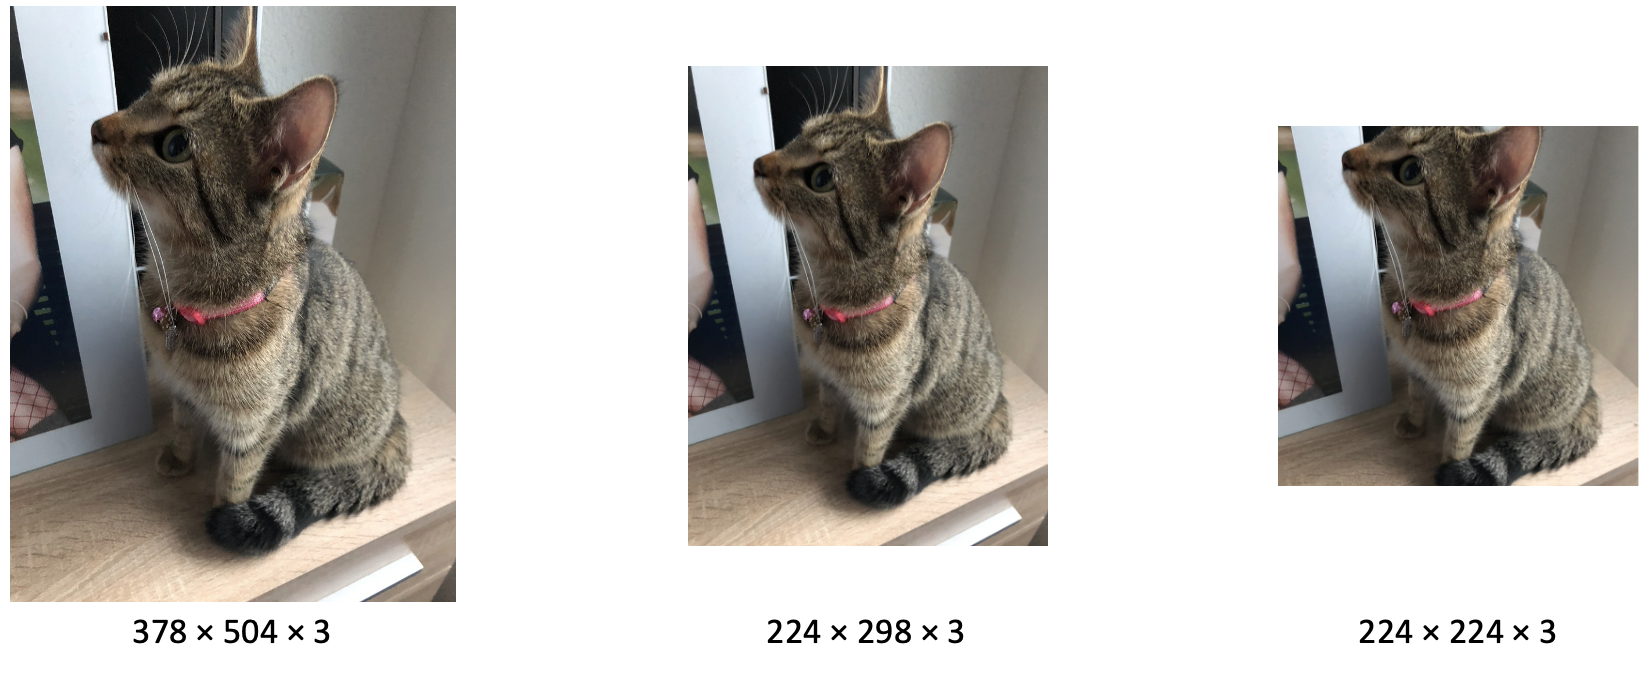
\includegraphics[width=\textwidth]{./images/image_resize.png}
\label{fig_preprocessing}
\end{figure}


Alle Modelle benötigen zusätzlich standardisierte Eingabewerte. 
Dafür wird von allen Farbkanal-Werten der mittlere Farbkanalwert aller Bilder aus dem Trainingsdatensatz subtrahiert. 
Die Channel-Werte sind so gleichmässig um $0$ verteilt. 
Für die Modelle Inception, ResNet-152, VGG-16 und VGG-19 wurde der Mittelwert aus \cite{martin_abadi_tensorflow_2015} verwendet. 
Für VGG-F wurde der zu \cite{chatfield_return_2014} veröffentlichte Mittelwert verwendet.






\chapter{Resultate Reproduktion}
\label{c_resultate_reprod}


\begin{table}[]
\centering
\caption{Störraten auf Trainings- und Validation-Set für die getesteten Modelle. Obere Reihen: $l_2$, $\xi=2000$, untere Reihen: $l_\infty$, $\xi=10$}
\begin{tabular}{|l|l|l|l|l|l|}
\hline

		            	& Inception	&	VGG-19		&	VGG-16		&	VGG-F	&	ResNet-152	\\ \hline
Trainings-Set, $l_2$		& $82.6\%$	&	$64.1\%$	&	$68.1\%$	&	$80.8\%$	& $79.5\%$	\\
Validation-Set, $l_2$ 			& $79.6\%$	&	$64.7\%$	&	$68.0\%$	&	$80.3\%$	& $80.9\%$	\\ \hline
Trainings-Set, $l_\infty$	& $86.3\%$	&	$54.5\%$	&	$59.2\%$	&	$89.8\%$	& $72.9\%$	\\
Validation-Set, $l_\infty$		& $81.9\%$	&	$54.7\%$	&	$59.5\%$	&	$89.6\%$	& $73.5\%$	\\

\hline 
\end{tabular}
\label{tbl_stoerraten_reprod}
\end{table}


Die erste Forschungsfrage dieser Thesis betrifft die Transferierbarkeit von mit UAP generierten Störwerten. Können die Ergebnisse aus der Originalarbeit \cite{moosavi-dezfooli_universal_2017-1} reproduziert werden?
Um diese Frage zu beantworten, wird UAP für die Testmodelle mit der gleichen Parameterkonfiguration wie in \cite{moosavi-dezfooli_universal_2017-1} beschrieben durchgeführt (siehe Abschnitt \ref{c_parameterwahl}).

In Tabelle \ref{tbl_stoerraten_reprod} sind die höchsten erreichten Störraten pro Modell und Datensatz aufgelistet. 
Fast alle darin aufgelisteten Störraten sind geringer als die von Moosavi-Dezfooli et al. in \cite{moosavi-dezfooli_universal_2017-1} publizierten Werte. 
Einzige Ausnahme ist der mit Inception generierte Störwert, begrenzt mit $l_\infty$-Norm.
In der Originalarbeit wurden in dieser Konfiguration $80.8\%$ auf dem Trainingsset und $78.9\%$ auf dem Validation-Set gemessen \cite{moosavi-dezfooli_universal_2017-1}.
Der reproduzierte Störwerte erreicht $86.3\%$ bzw. $81.9\%$ auf Trainings- und Validation-Set. Dies entspricht einer absoluten Veränderung von $3.0\%$ bzw. $5.5\%$. Für die Netzwerke VGG-F und ResNet-152 konnten hohe Störraten erreicht werden, diese sind aber $3.9\%$ bis $12.5\%$ geringer als in der Originalarbeit. 
Für die Netzwerke VGG-16 und VGG-19 sind die Störraten über $20\%$ schlechter. 
Sie konnten im Vergleich zu den anderen drei Netzwerken bedeutend schlechter gestört werden. 

\pagebreak

Auffallend ist, dass einige Störwerte auf dem Validation-Set eine höhere Störrate erreichen als auf dem zum Generieren verwendeten Trainingsset (z.B. ResNet-152). Dieses Verhalten wurde von Moosavi-Dezfooli et al. in ihrer Arbeit \cite{moosavi-dezfooli_universal_2017-1} ebenfalls gemessen. Eine mögliche Erklärung dafür ist die Verteilung der Klassen im Trainingsset. Das Trainingsset könnte prozentual mehr schwer zu störende Bilder beinhalten als das Validation-Set. In diesem Fall wäre das Validation-Set anfälliger auf den Störwert als das Trainingsset selbst.

\pagebreak

\section{Transferierbarkeit der Störwerte}
\label{c_resultate_transferierbarkeit}

\begin{table}[]
\centering
\caption{Störraten auf Validation-Set. Oben: Modell, mit dem Störwert generiert wurde, links: angegriffenes Modell ($l_2$, $\xi=2000$)}
\begin{tabular}{|l|l|l|l|l|l|}
\hline

			& VGG-F		&	Inception	&	VGG-16		&	VGG-19		&	ResNet-152	\\ \hline
VGG-F		& $80.3\%$	&	$17.5\%$		&	$19.3\%$		&	$17.3\%$		& 	$29.8\%$	\\
Inception	& $40.6\%$	&	$79.6\%$		&	$34.6\%$		&	$29.3\%$		& 	$33.3\%$	\\
VGG-16		& $18.3\%$	&	$11.8\%$		&	$67.9\%$		&	$49.4\%$		& 	$17.9\%$	\\
VGG-19		& $18.0\%$	&	$11.8\%$		&	$51.3\%$		&	$64.7\%$		& 	$17.3\%$	\\
ResNet-152	& $18.1\%$	&	$13.4\%$		&	$18.8\%$		&	$16.3\%$		& 	$80.9\%$	\\

\hline 
\end{tabular}
\label{tbl_stoerraten_reprod_kreuz_l2}
\end{table}

\begin{table}[]
\centering
\caption{Störraten auf Validation-Set. Oben: Modell mit dem Störwert generiert wurde, links: angegriffenes Modell ($l_\infty$, $\xi=10$)}
\begin{tabular}{|l|l|l|l|l|l|}
\hline

			& VGG-F		&	Inception		&	VGG-16		&	VGG-19			&	ResNet-152	\\ \hline
VGG-F		& $89.6\%$	&	$25.1\%$		&	$46.2\%$	&	$45.1\%$			& 	$42.4\%$		\\
Inception	& $56.5\%$	&	$81.9\%$		&	$59.9\%$	&	$57.5\%$		& 	$54.6\%$	\\
VGG-16		& $32.4\%$	&	$15.9\%$		&	$58.7\%$	&	$50.6\%$		& 	$31.4\%$	\\
VGG-19		& $32.2\%$	&	$15.8\%$		&	$51.9\%$	&	$54.3\%$		& 	$30.1\%$	\\
ResNet-152	& $24.4\%$	&	$15.6\%$		&	$38.0\%$	&	$33.4\%$		& 	$73.4\%$	\\

\hline 
\end{tabular}
\label{tbl_stoerraten_reprod_kreuz_linf}
\end{table}

Um Referenzwerte für die zweite Forschungsfrage zu erhalten, wird die Transferierbarkeit der Störwerte auf andere Modellen gemessen. 
Auch bei der Transferierbarkeit auf andere Modelle zeigen sich Unterschiede zu den von Moosavi-Dezfooli et al. gemessenen Werten.

In Tabelle \ref{tbl_stoerraten_reprod_kreuz_l2} ist ersichtlich, wie die Störwerte andere Modelle beeinflussen. 
Die Störwerte erreichen auf anderen Modellen in den meisten Fällen eine Störrate zwischen $10\%$ bis $20\%$. 
Ausnahmen sind die Störwerte des Inception-Modells, welches auf den anderen Modellen Störraten von $29.3\%$ bis $40.6\%$ erreicht. 
Ebenfalls eine höhere Störrate erzielen die mit VGG-16 und VGG-19 generierten Störwerte, welche auf dem jeweils anderen VGG-Netz eine Störrate von $51.3\%$ bzw. $49.4\%$ erreichen.

Mit anderem Distanzmass und maximaler Norm ($l_\infty$, $\xi=10$) ändert sich die Transferierbarkeit auf andere Modelle. 
Die Konfiguration $l_\infty$, $\xi=10$ generiert Störwerte, die besser auf andere Modelle übertragbar sind. 
Bemerkenswert ist dabei die Störrate eines mit VGG-16 erstellten Störwertes, der beim Inception-Modell eine Störrate von $59.9\%$ erreicht (siehe Tabelle \ref{tbl_stoerraten_reprod_kreuz_linf}). 
Dieser Störwert kann das Inception-Modell besser stören, als das zum Generieren verwendete VGG-16. 
Das Inception-Modell kann mit dieser Parameter-Wahl mit allen Störwerten zu $54.6\%$ bis $59.9\%$ gestört werden. 
Auch die anderen Modelle sind in dieser Parameterkonfiguration anfälliger auf Störwerte anderer Modelle. 

Die gemessenen Störraten sind dennoch tiefer, als die von Moosavi-Dezfooli et al. gemessenen Störraten. 
So konnte in ihren Tests ein mit Inception generierter Störwert auf anderen Modellen Störraten von $39.2\%$ bis $46.2\%$ erreichen. 
Die reproduzierten Störwerte erreichen mit einem Inception-Störwert nur $15.6\%$ bis $25.1\%$.

\section{Visueller Vergleich}


\begin{figure}[h]

\caption{Mit verschiedenen Modellen errechnete Störwerte. Zur Visualisierung wurden die Farbkanal-Werte um $\xi$ in die positive Richtung verschoben und mit $2\xi / 255$ multipliziert.}
\centering
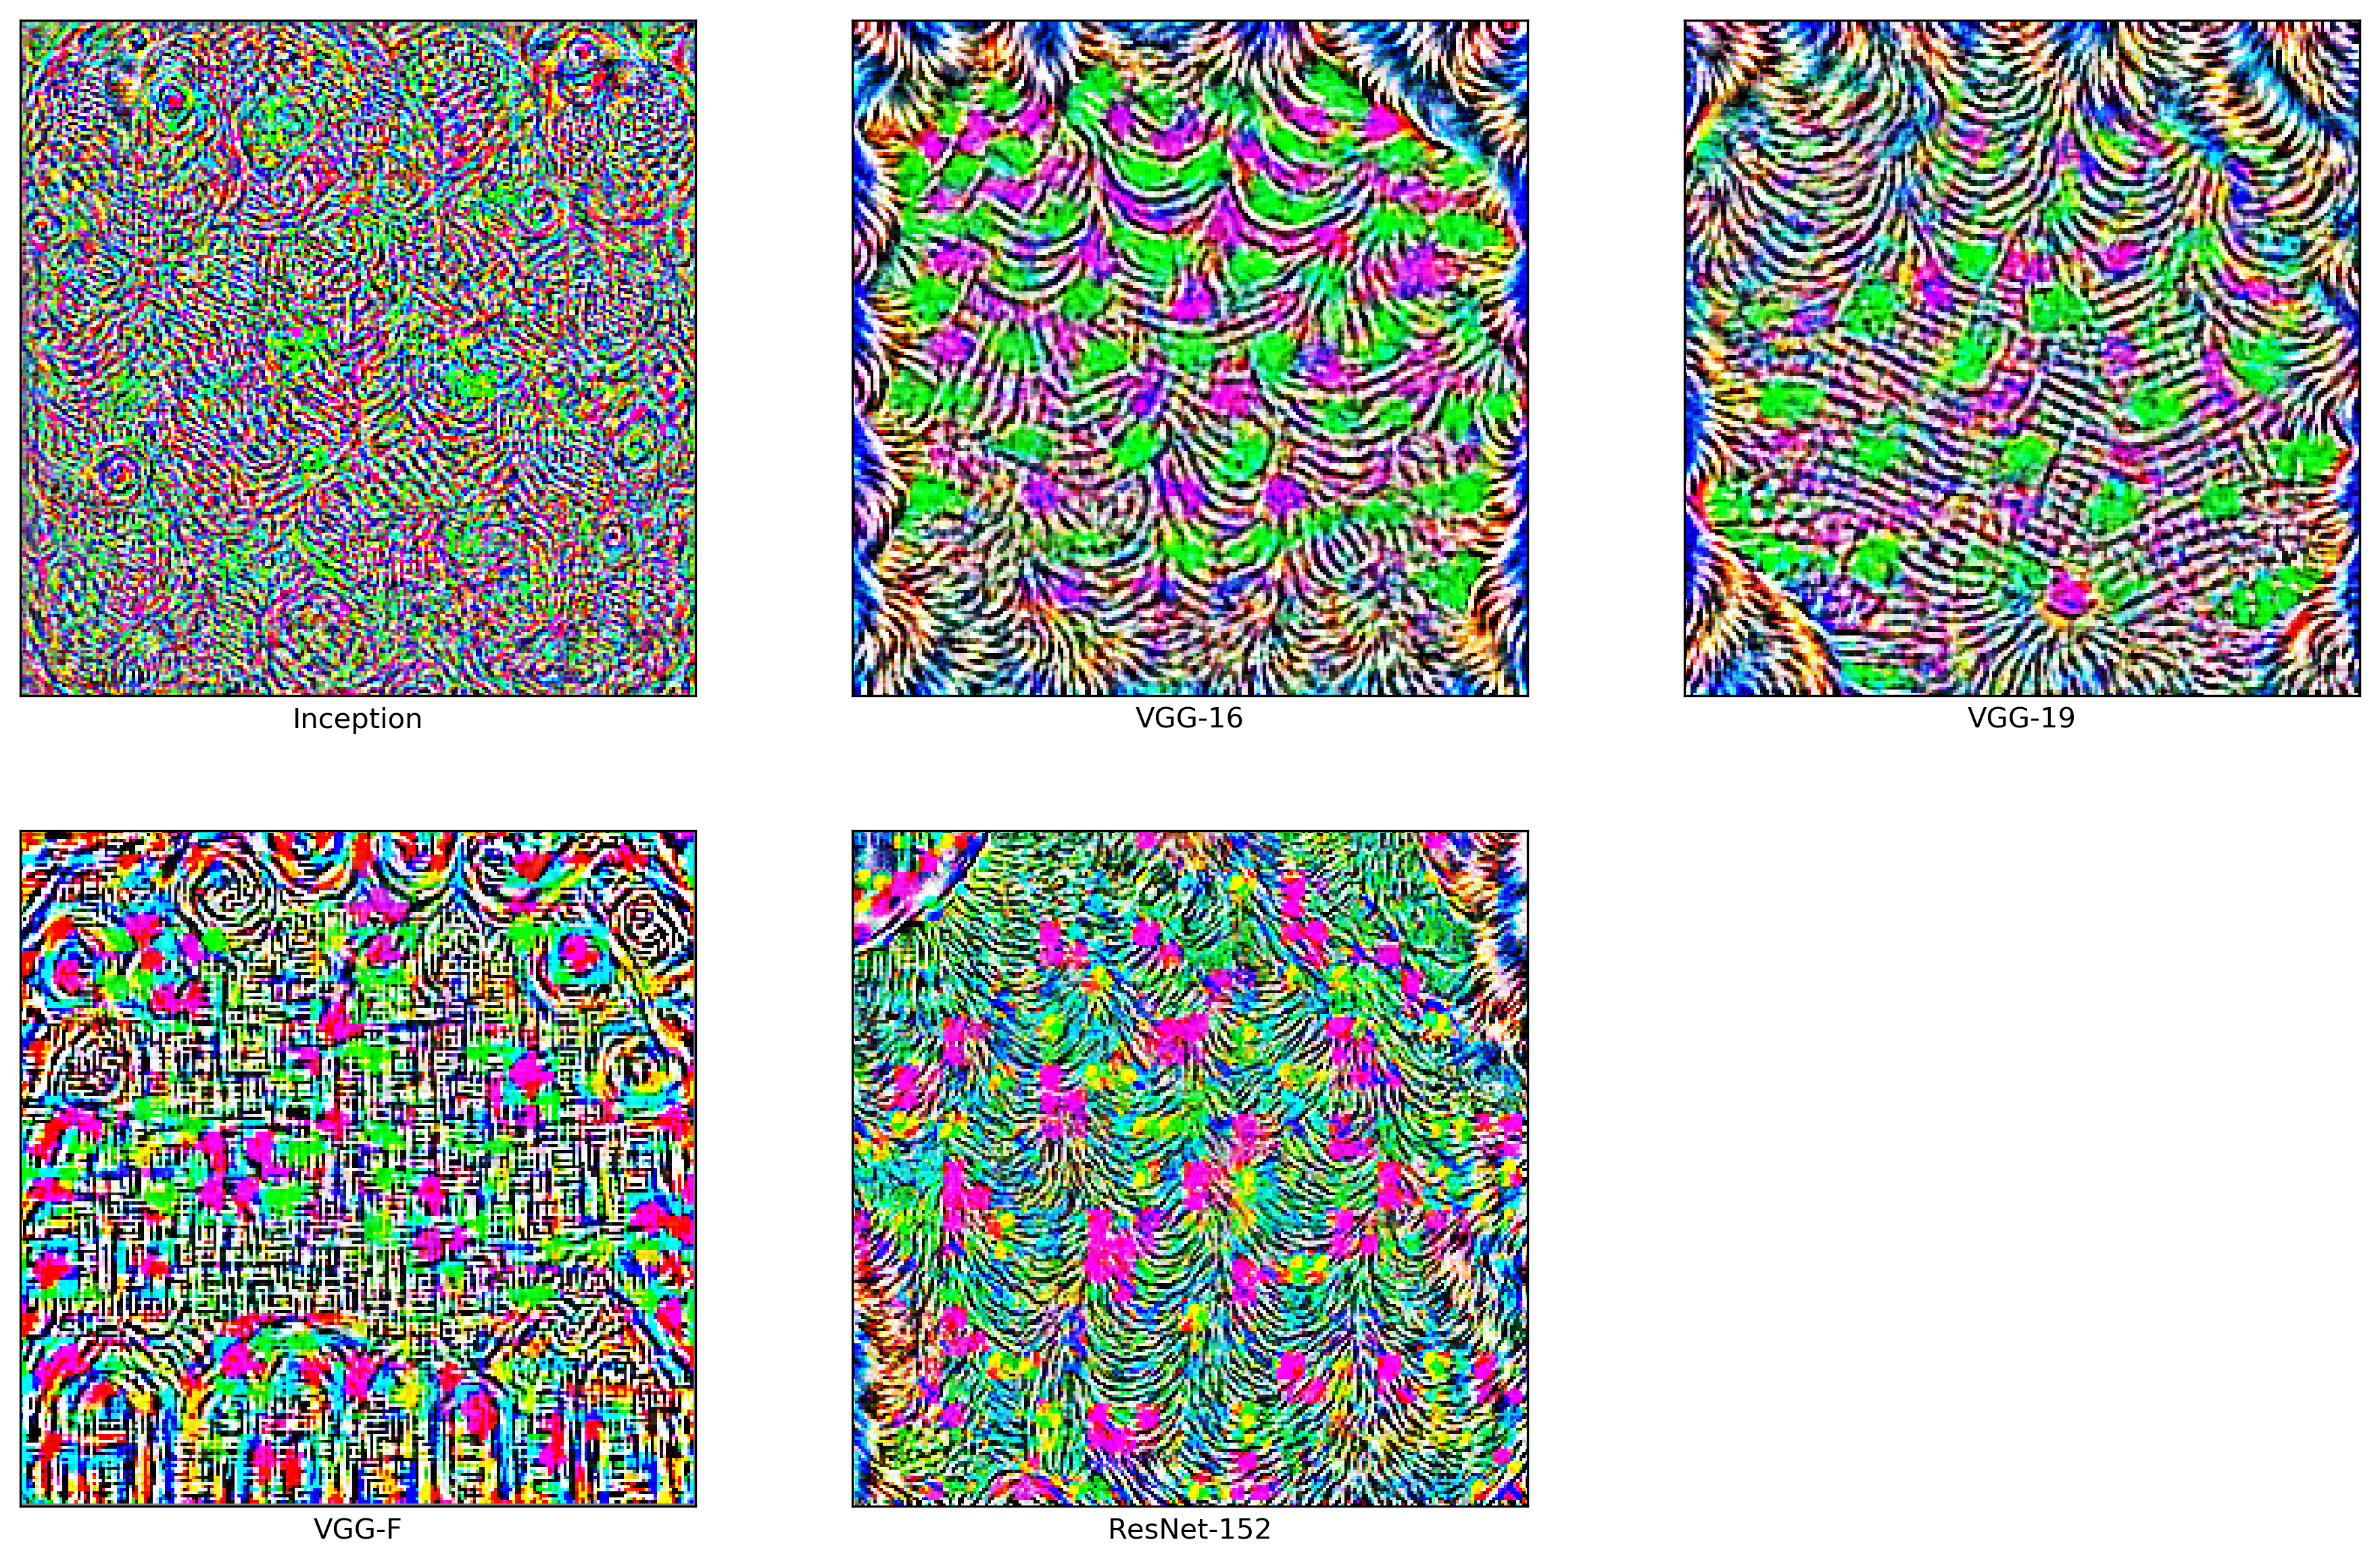
\includegraphics[width=\textwidth]{./images/own_perturbations.png}
\label{fig_stoerwerte}
\end{figure}


Um eine Erklärung für die Unterschiede der Störungsraten zu finden, werden die Störwerte visuell untersucht. 
In Abbildung \ref{fig_stoerwerte} sind die reproduzierten Störwerte visualisiert ($l_\infty$, $\xi=10$). 
Die Störwerte zeigen ähnliche Strukturen wie die Störwerte aus \cite{moosavi-dezfooli_universal_2017-1}. 
Insbesondere sind pro Modell einzigartige Strukturen erkennbar. 
Modelle mit einer ähnlichen Modellstruktur haben auch ähnliche Störwerte (siehe VGG-16 und VGG-19).

Auffallend bei diesen Strukturen ist, dass einige der Störwerte unterschiedliche Muster am Rand und Zentrum aufweisen und nicht symmetrisch sind. Die Modelle klassifizieren aber unabhängig von der Objektlokation im Bild. Dieses Muster könnte auf die gewählten Trainingsdaten der Modelle zurückzuführen sein. Die Trainingsdaten könnten eine Tendenz dazu haben, dass das zu klassifizierende Objekt sich in der Mitte des Bildes befindet. Entsprechend sind die Ränder der Bilder weniger relevant für die (Falsch-) Klassifikation.

Im Vergleich zu den in \cite{moosavi-dezfooli_universal_2017-1} abgebildeten Störwerten haben die reproduzierten Störwerte weichere Konturen und erscheinen heller. 
Da nicht bekannt ist, wie in \cite{moosavi-dezfooli_universal_2017-1} die Bilder visualisiert wurden, kann dies durch unterschiedliche Visualisierungsmethoden entstanden sein.



\section{Verlauf der Störrate über mehrere Iterationen}

\begin{figure}[h]
\caption{Störraten auf Trainingsset (links) und Validation-Set (rechts) über $20$ UAP-Iterationen}
\centering
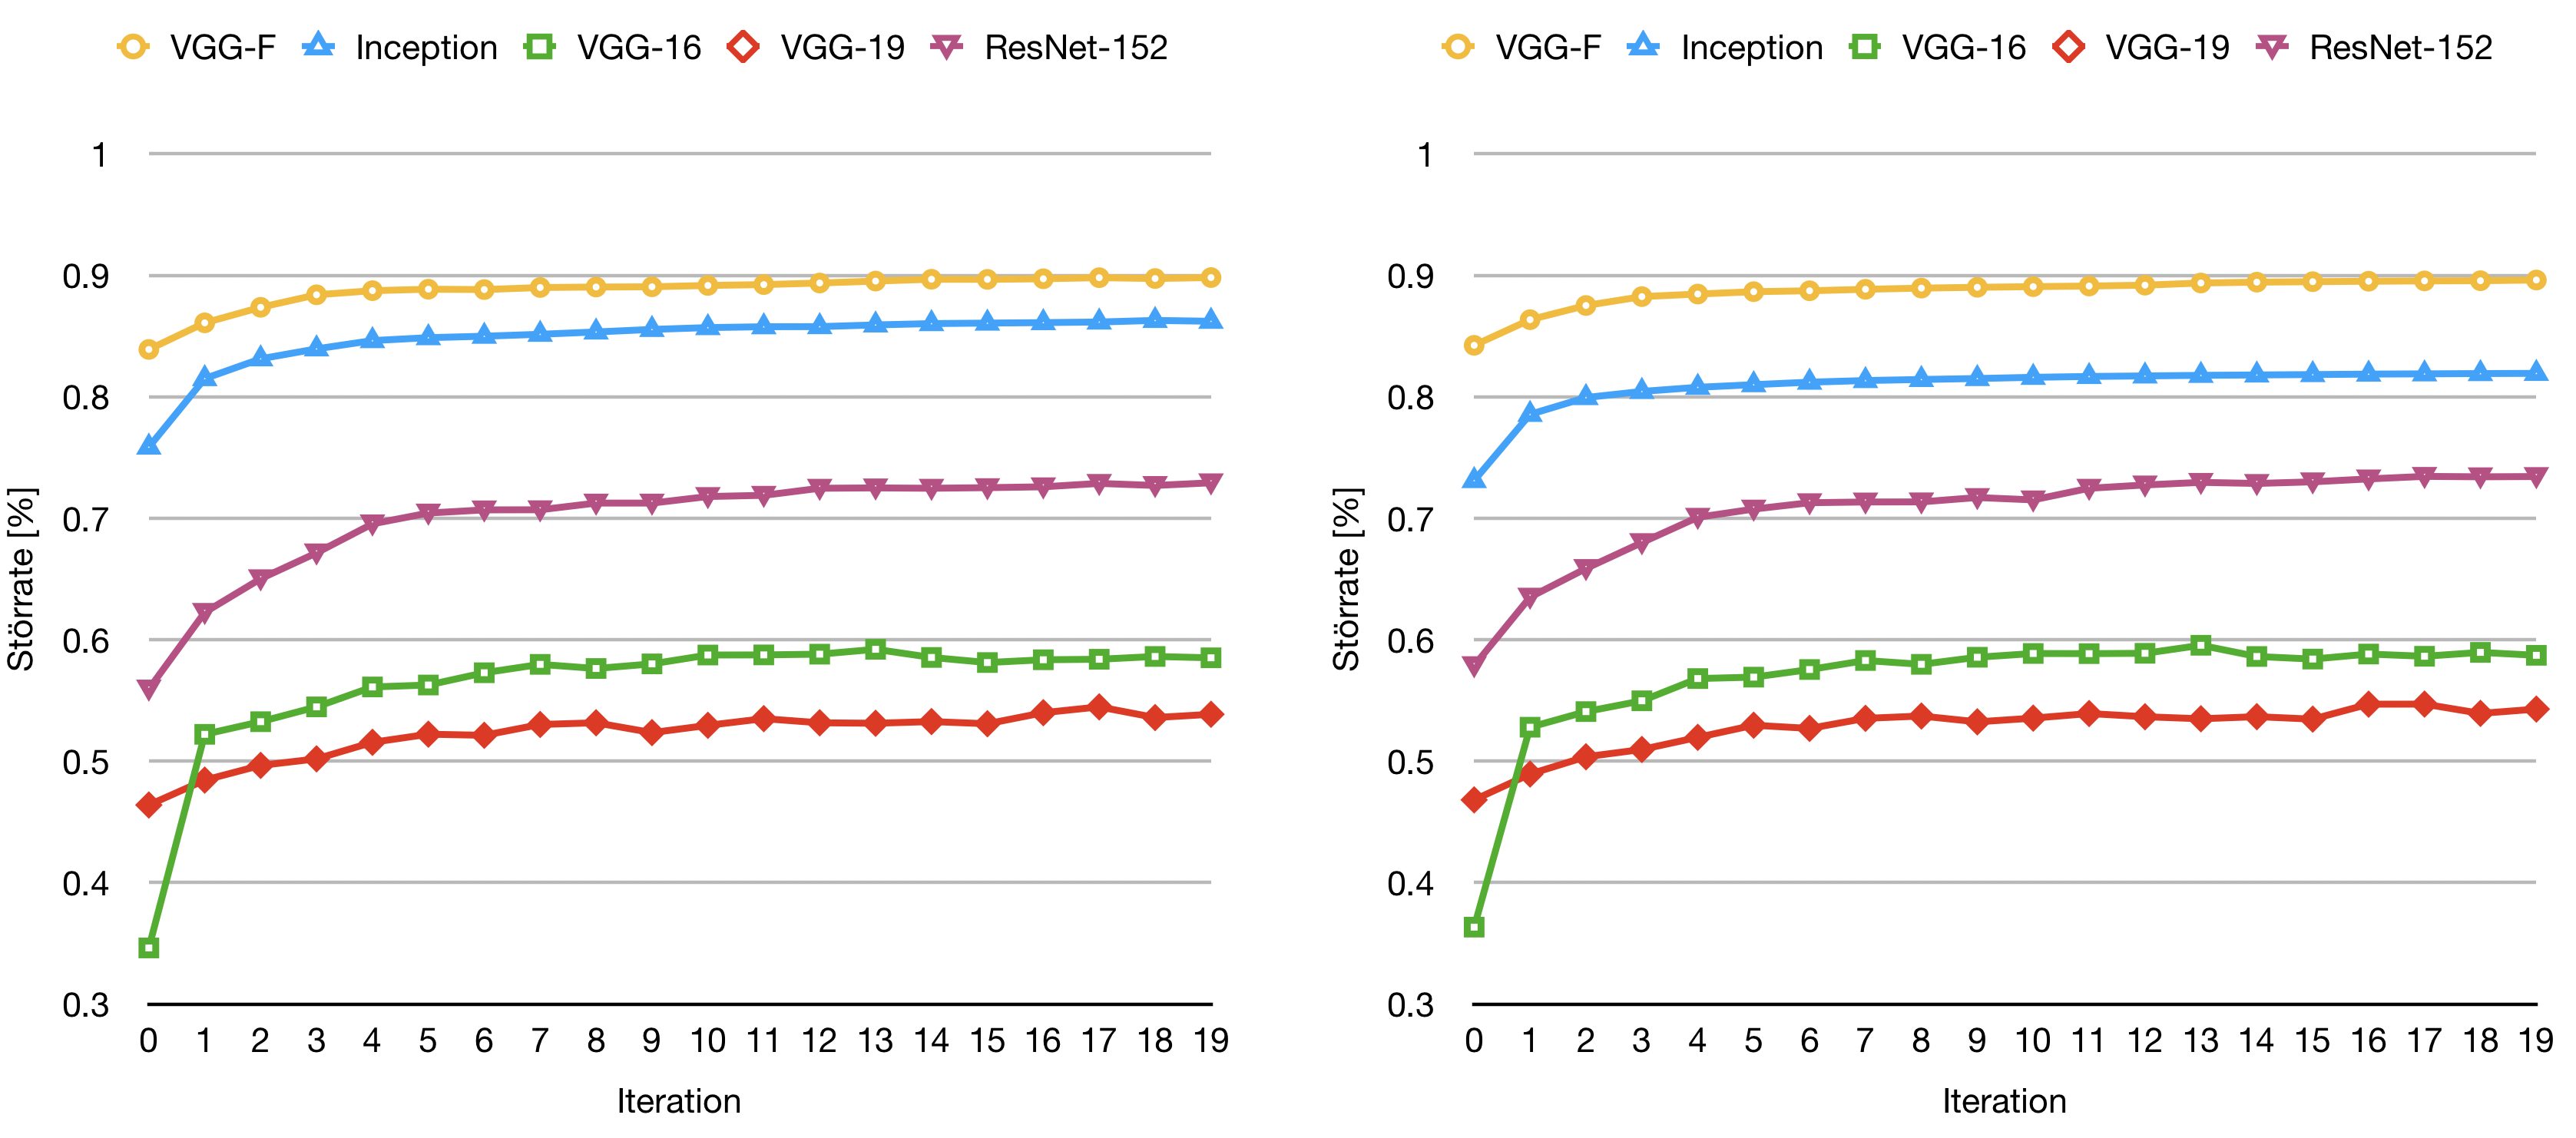
\includegraphics[width=\textwidth]{./images/stoerraten_training.png}
\label{fig_stoerrate_iterationen}
\end{figure}

Eine Erklärung für die tieferen Störraten wäre, wenn das Verfahren mit zu wenigen Iterationen durchgeführt wurde. 
In der Reproduktion wurde das von Moosavi-Dezfooli et al. beschriebene Stoppkriterium durch eine fixe Anzahl durchgeführter Iterationen ersetzt. 
Um das zu untersuchen, wird die Veränderung der Störraten über die $20$ UAP-Iterationen hinweg auf Trainings- und Validation-Set untersucht. 
Sofern die Störrate sich weiterhin verbessert, würde das die tieferen Störraten erklären.

Die Störraten sind in Abbildung \ref{fig_stoerrate_iterationen} visualisiert. 
Unabhängig vom Modell nähert sich die Störrate nach wenigen Iterationen bereits der besten gemessenen Störrate an.
Weitere Iterationen verbessern das Ergebnis nur noch geringfügig. Dieses Verhalten lässt vermuten, dass weitere UAP-Iterationen die Störraten nicht weiter verbessern.

Die Störraten unterscheiden sich zwischen Trainings- und Validation-Set nur gering ($\leq5\%$ Unterschied). 
Auch nicht zum Training verwendete Bilder lassen sich mit den Störwerten stören. Die Störwerte sind also universell, bzw. unabhängig vom zu störenden Bild.



\section{Einfluss weiterer Parameter auf die Störrate}

Eine weitere Erklärung für die tieferen Störraten könnten die in \cite{moosavi-dezfooli_universal_2017-1} nicht beschriebenen Parameter für DeepFool sein. 
Andere Parameterwerte verändern den generierten Störwert und damit auch die erzielte Störrate.
Die Veränderung der Störrate durch diese Parameter wurde anhand des VGG-16-Modells gemessen.

\subsection{Anzahl getesteter Klassen}

Die Anzahl getesteter Klassen definiert für DeepFool, von wie vielen Klassen die Distanz zur Klassengrenze gemessen wird. 
Für die Resultate in der Tabelle \ref{tbl_stoerraten_reprod} wurden $10$ Klassen getestet, der ImageNet-Datensatz beinhaltet aber $1'000$ Klassen. 
Es wäre möglich, dass es eine nicht getestete Klasse mit kleinerer Distanz zur Klassengrenze gibt. 
Da diese nicht geprüft wird, muss DeepFool einen grösseren Störwert erzeugen. 
Das wiederum kann sich negativ auf den UAP-Störwert auswirken, da dieser die definierte Norm $\xi$ nicht übersteigen darf.

Um die Auswirkung der Anzahl getesteter Klassen zu prüfen, werden Störwerte mit $50$, $100$ und $200$ getesteten Klassen berechnet. 
Es wurden keine Tests für mehr als $200$ Klassen durchgeführt, da die Ausführzeit und der Arbeitsspeicherbedarf mit jeder zu testenden Klasse ansteigt. 
Mit den verfügbaren Ressourcen konnten diese Tests nicht durchgeführt werden. 
Die Störraten über $10$ UAP-Iterationen auf VGG-16 sind in Abbildung \ref{fig_einfluss_num_cls} visualisiert.

Mit $50$ getesteten Klassen konnte ein $4\%$ besseres Ergebnis erzielt werden, als mit $10$ getesteten Klassen. 
Tests mit noch mehr Klassen ($100$, $200$) ergaben zwar ebenfalls bessere Ergebnisse, die Störrate stieg aber nur um $1.1\%$ bzw. $1.8\%$. 
Die Anzahl getesteter Klassen scheint nur einen geringen Einfluss auf die Störrate des eigentlichen Modells zu haben. 
Da keine Tests mit allen Klassen durchgeführt wurden, kann diese Vermutung aber nicht bestätigt werden.

\begin{figure}[h]
\caption{VGG-16 Störraten auf Validation-Set mit unterschiedlicher Anzahl getesteter Klassen in DeepFool}
\centering
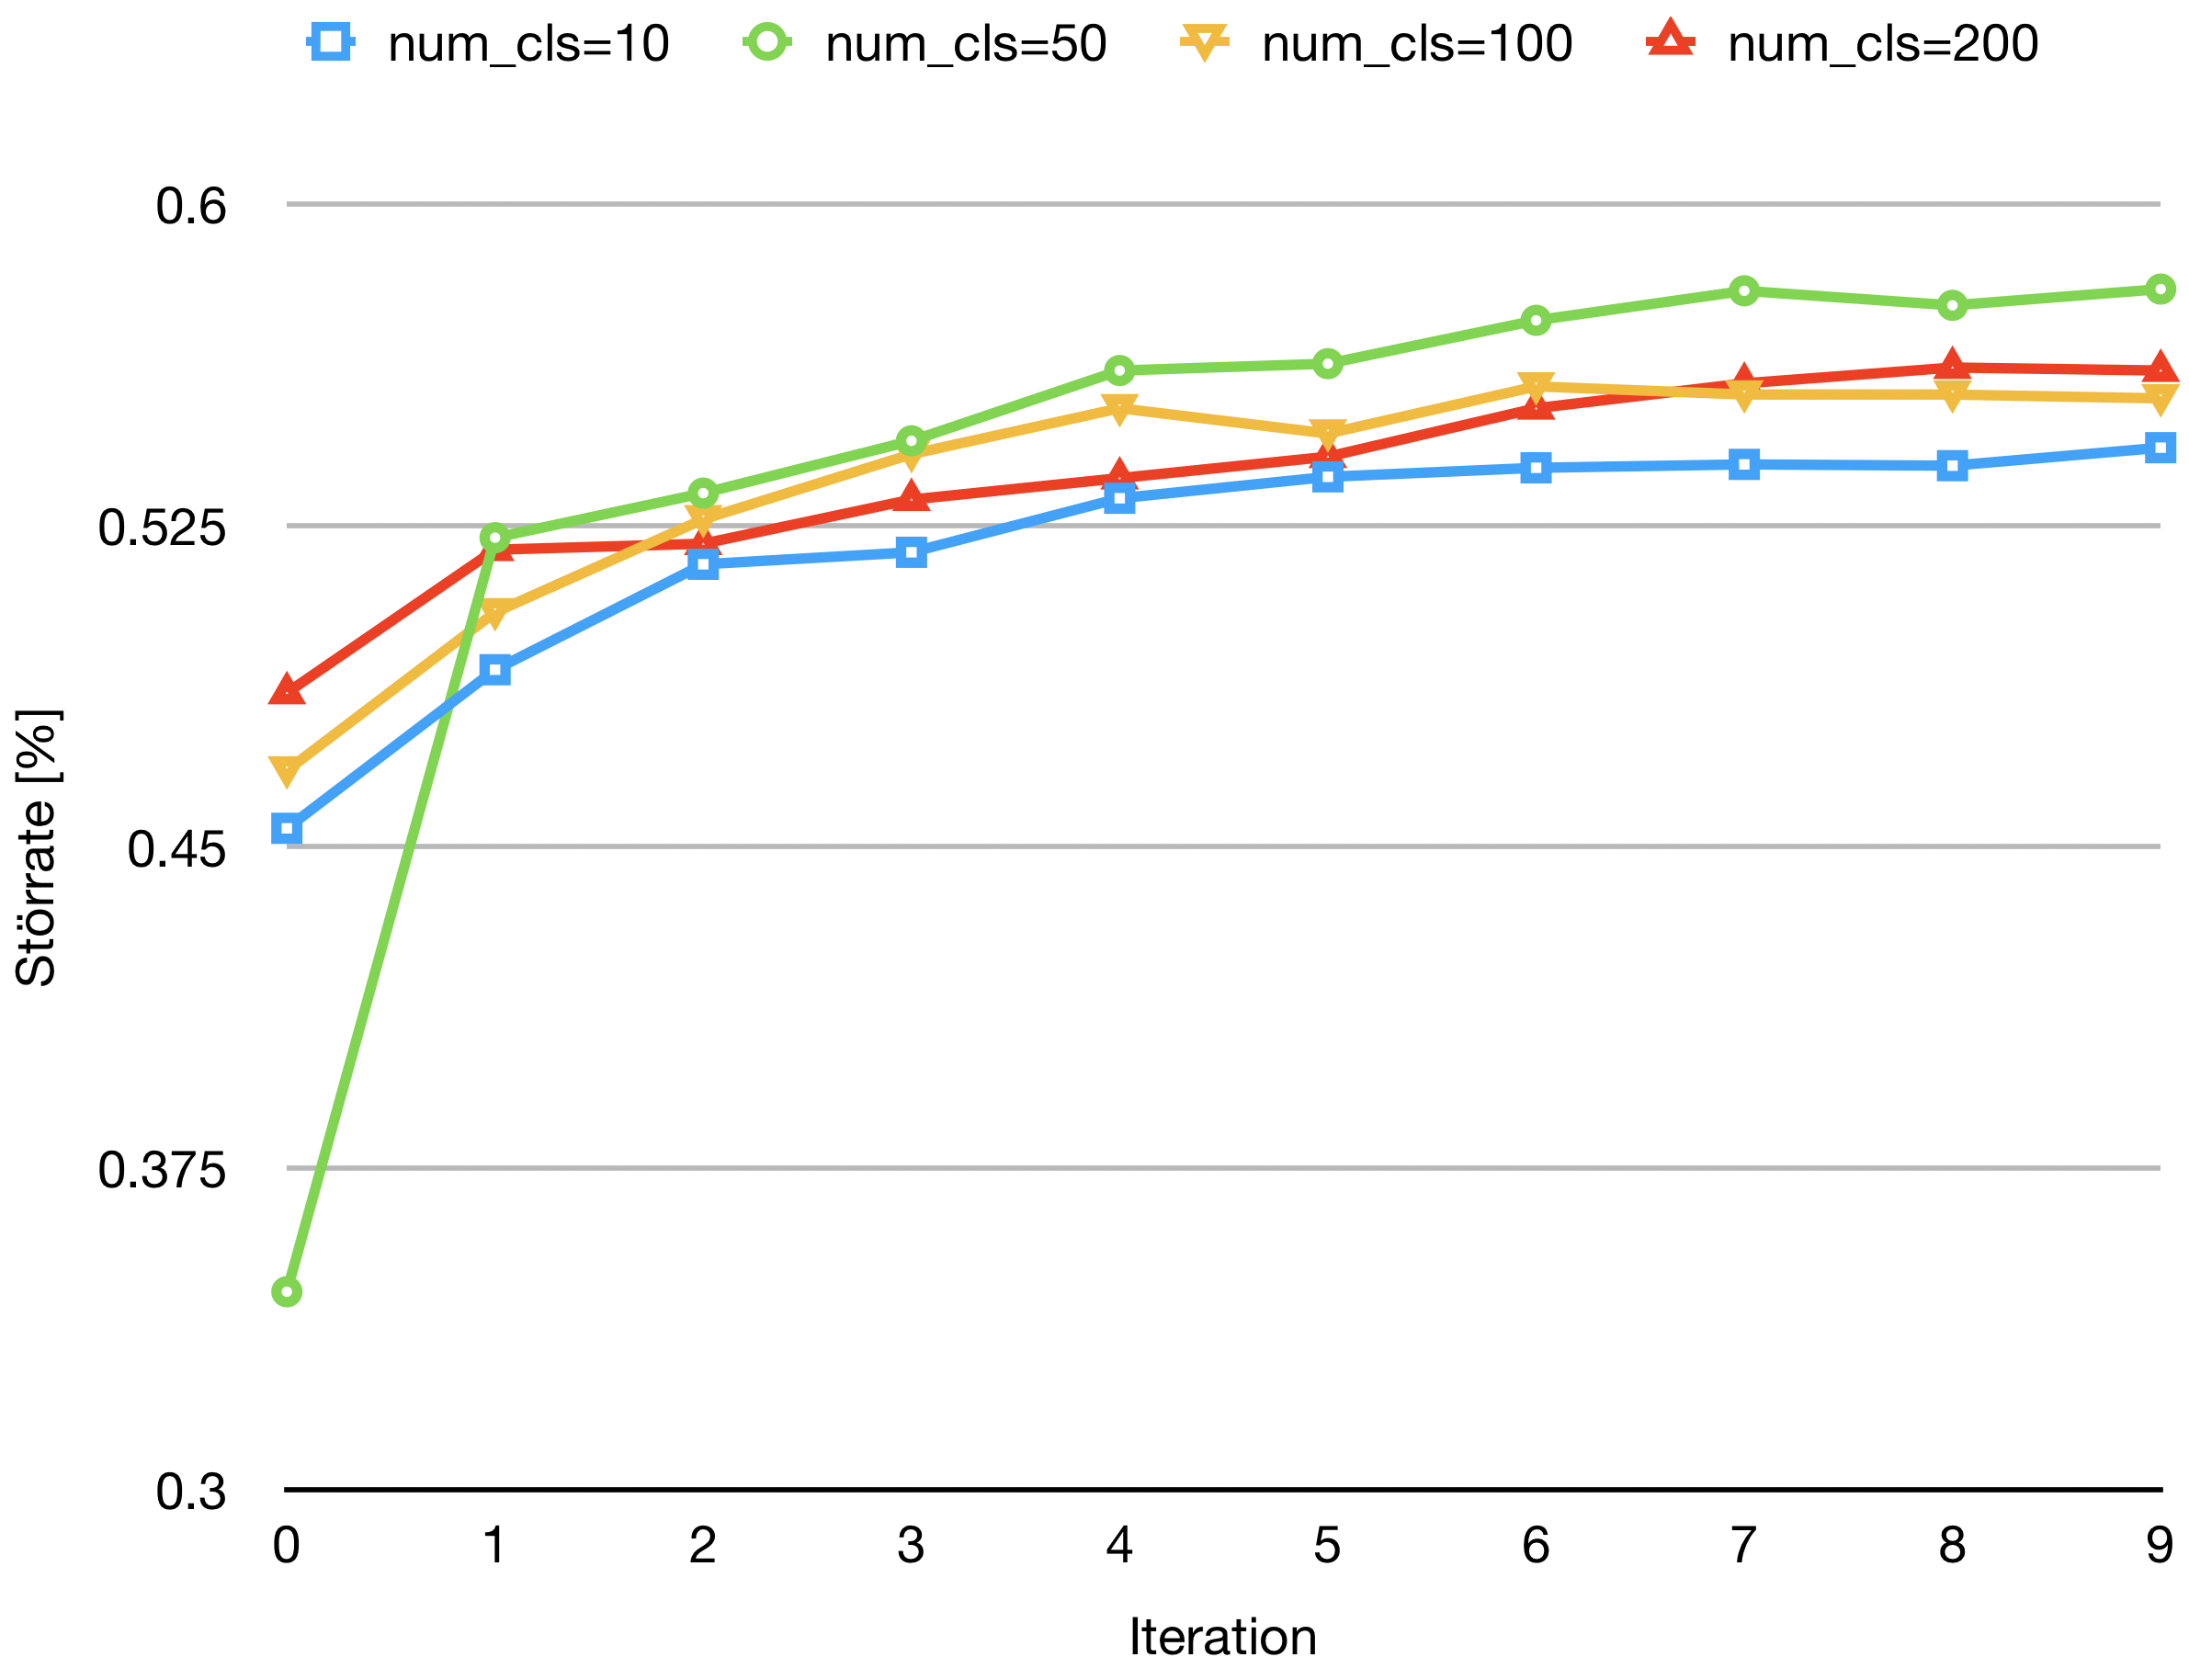
\includegraphics[width=0.7\textwidth]{./images/einfluss_num_cls.png}
\label{fig_einfluss_num_cls}
\end{figure}



\subsection{Überschuss ($\eta$)}

\begin{figure}[h]
\caption{VGG-16-Störraten auf Validation-Set mit verschiedenen $\eta$-Werten}
\centering
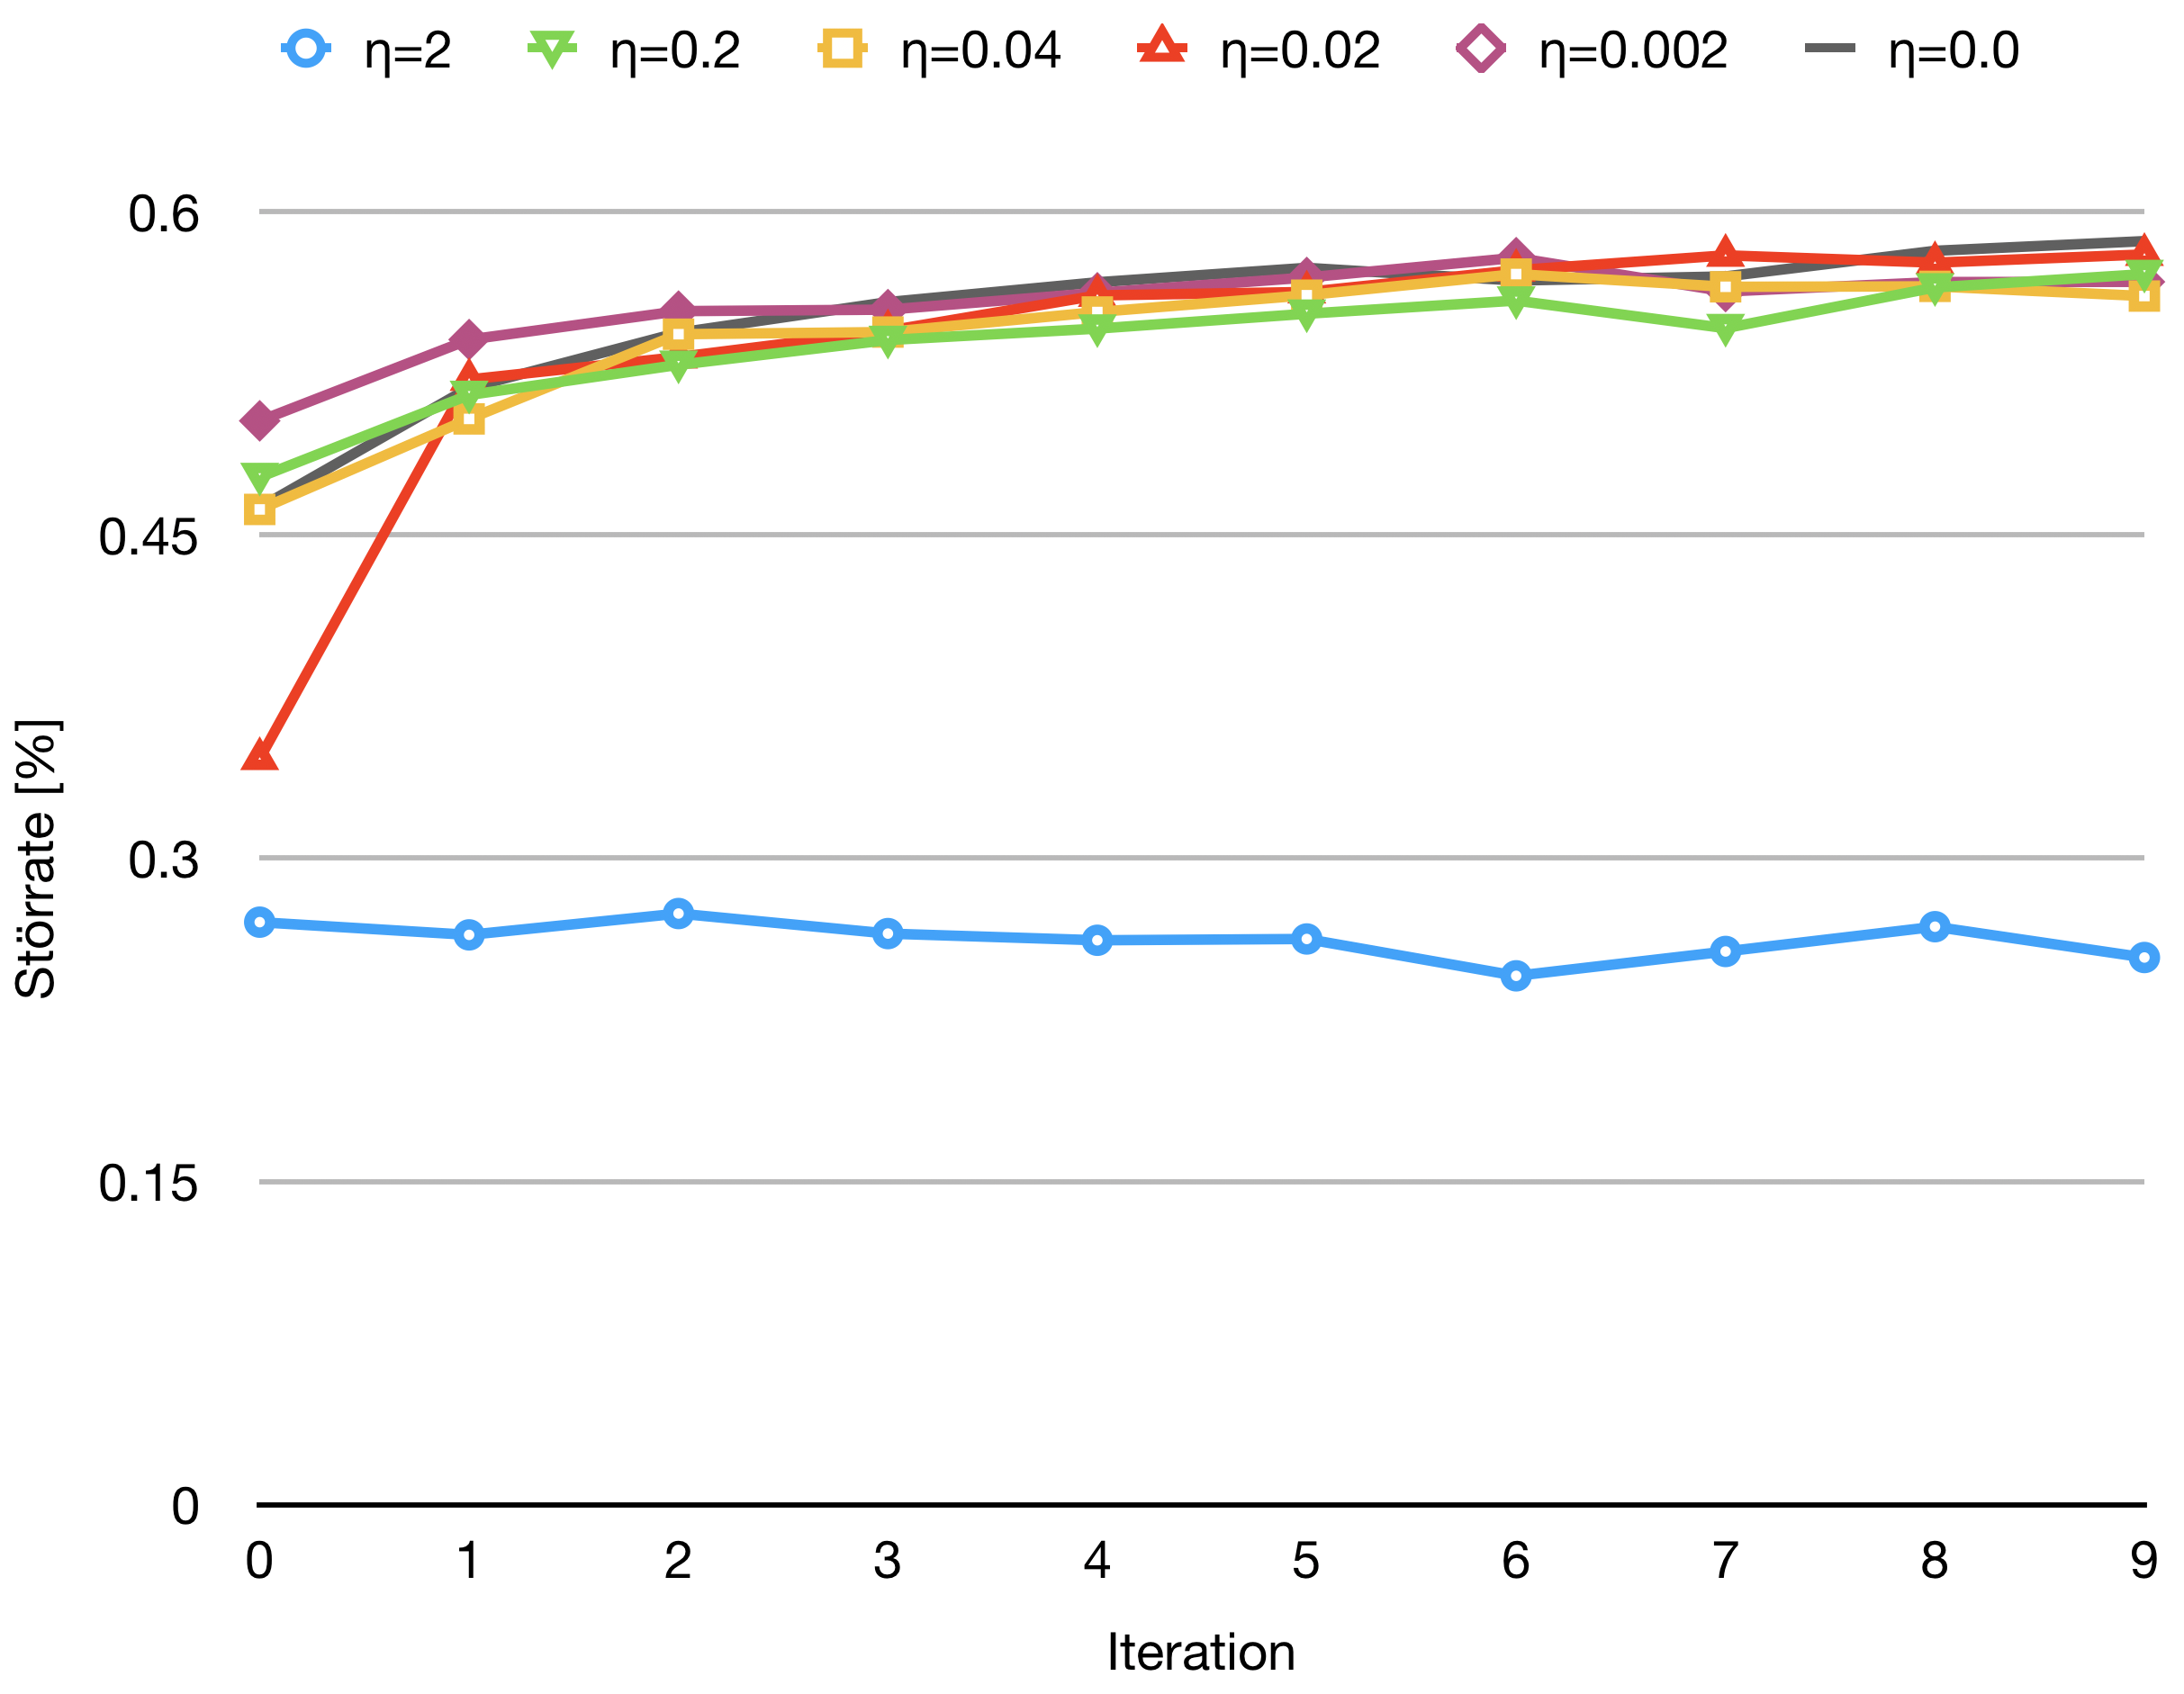
\includegraphics[width=0.7\textwidth]{./images/einfluss_eta.png}
\label{fig_einfluss_eta}
\end{figure}


Nachdem DeepFool eine Klassengrenze gefunden hat, wird der Störwert mit $1+\eta$ multipliziert. 
Damit soll der Störwert minimal vergrössert werden, damit die Klassengrenze sicher überschritten wird. 
Bei diesem Parameter gibt es zwei Varianten, wie der Parameter den Störwert negativ beeinflussen kann. 
Mit zu grossem $\eta$ entsteht für jedes einzelne Bild ein grösserer Störwert. 
Aufgrund der Normierung auf $\xi$ führt dies wiederum zu einem schlechteren UAP-Störwert.

Wird $\eta$ zu klein gewählt, kann der Störwert das Bild u.U. gar nicht stören, da man sich der Klassengrenze nur annähert, statt sie effektiv zu überschreiten.

Es wurden $5$ verschiedene Werte für $\eta$ mit VGG-16 getestet, um dessen Einfluss auf die Störrate zu messen. 
In Abbildung \ref{fig_einfluss_eta} sind die Störraten über $10$ UAP-Iterationen visualisiert. 
Der Wert von $\eta$ hat nur minimalen Einfluss auf die erzielte Störrate, sofern ein Wert $\ll 1$ verwendet wird (wie in \cite{moosavi-dezfooli_deepfool_2016} beschrieben). 
Mit $\eta=0.0$ wurde die beste Störrate erreicht ($58.6\%$). 
Damit wurde eine $0.5\%$ bessere Störrate erreicht als mit dem Originalwert $\eta=0.02$. 
Dies ist beachtenswert, da gem. Moosavi-Dezfooli et al. ein $\eta > 0$ in einigen Fällen notwendig ist, um die Klassengrenze zu überschreiten \cite{moosavi-dezfooli_deepfool_2016}. Dies scheint bei VGG-16 nur selten aufzutreten.


\subsection{Maximale Anzahl DeepFool-Iterationen}

DeepFool wird nach maximal $i_d$ Iterationen abgebrochen. 
Wurde diese Anzahl Iterationen erreicht, konnte für das Bild kein Störwert errechnet werden. 
Das Ergebnis von DeepFool wird in diesem Fall nicht zum UAP-Störwert hinzugefügt. 
Wenn dies bei vielen Bildern eintritt, kann der UAP-Störwert diese Bilder ebenfalls nicht stören. Der Störwert kann nicht mehr optimiert werden. Dieser Fall könnte erklären, warum die Störrate bereits nach einigen Iterationen nur noch minimal besser wird. 

Um den Einfluss dieses Parameters zu messen, werden Störwerte für VGG-16 und VGG-F generiert. Während dem Generieren wird für jede Iteration gezählt, wie oft DeepFool keinen Störwert für ein einzelnes Bild finden konnte. VGG-F wurde als zweites Modell gewählt, da für dieses Modell im Gegensatz zu VGG-16 ohne Modifikation der Parameter eine hohe Störrate erreicht wurde.

 Während $10$ Iterationen mit je $10'000$ Bildern wurde gemessen, wie oft DeepFool abgebrochen wurde. Für VGG-F trat der Fall in $3$ Iterationen ein, für VGG-16 in $2$ Iterationen. Bei VGG-F konnten über alle Iterationen $5$ Bilder nicht gestört werden, bei VGG-16 waren es $2$ Bilder. Die Einschränkung der maximalen Anzahl DeepFool-Iterationen auf $10$ hat also keinen negativen Einfluss auf die mit UAP generierten Störwerte. Es wurden deshalb keine Tests mit höheren $i_d$-Werten durchgeführt.

\subsection{Datenset}



\begin{figure}[h]
\caption{Störrate auf Validation-Set auf VGG-16 mit ausgeglichenem und zufälligem Trainingsset}
\centering
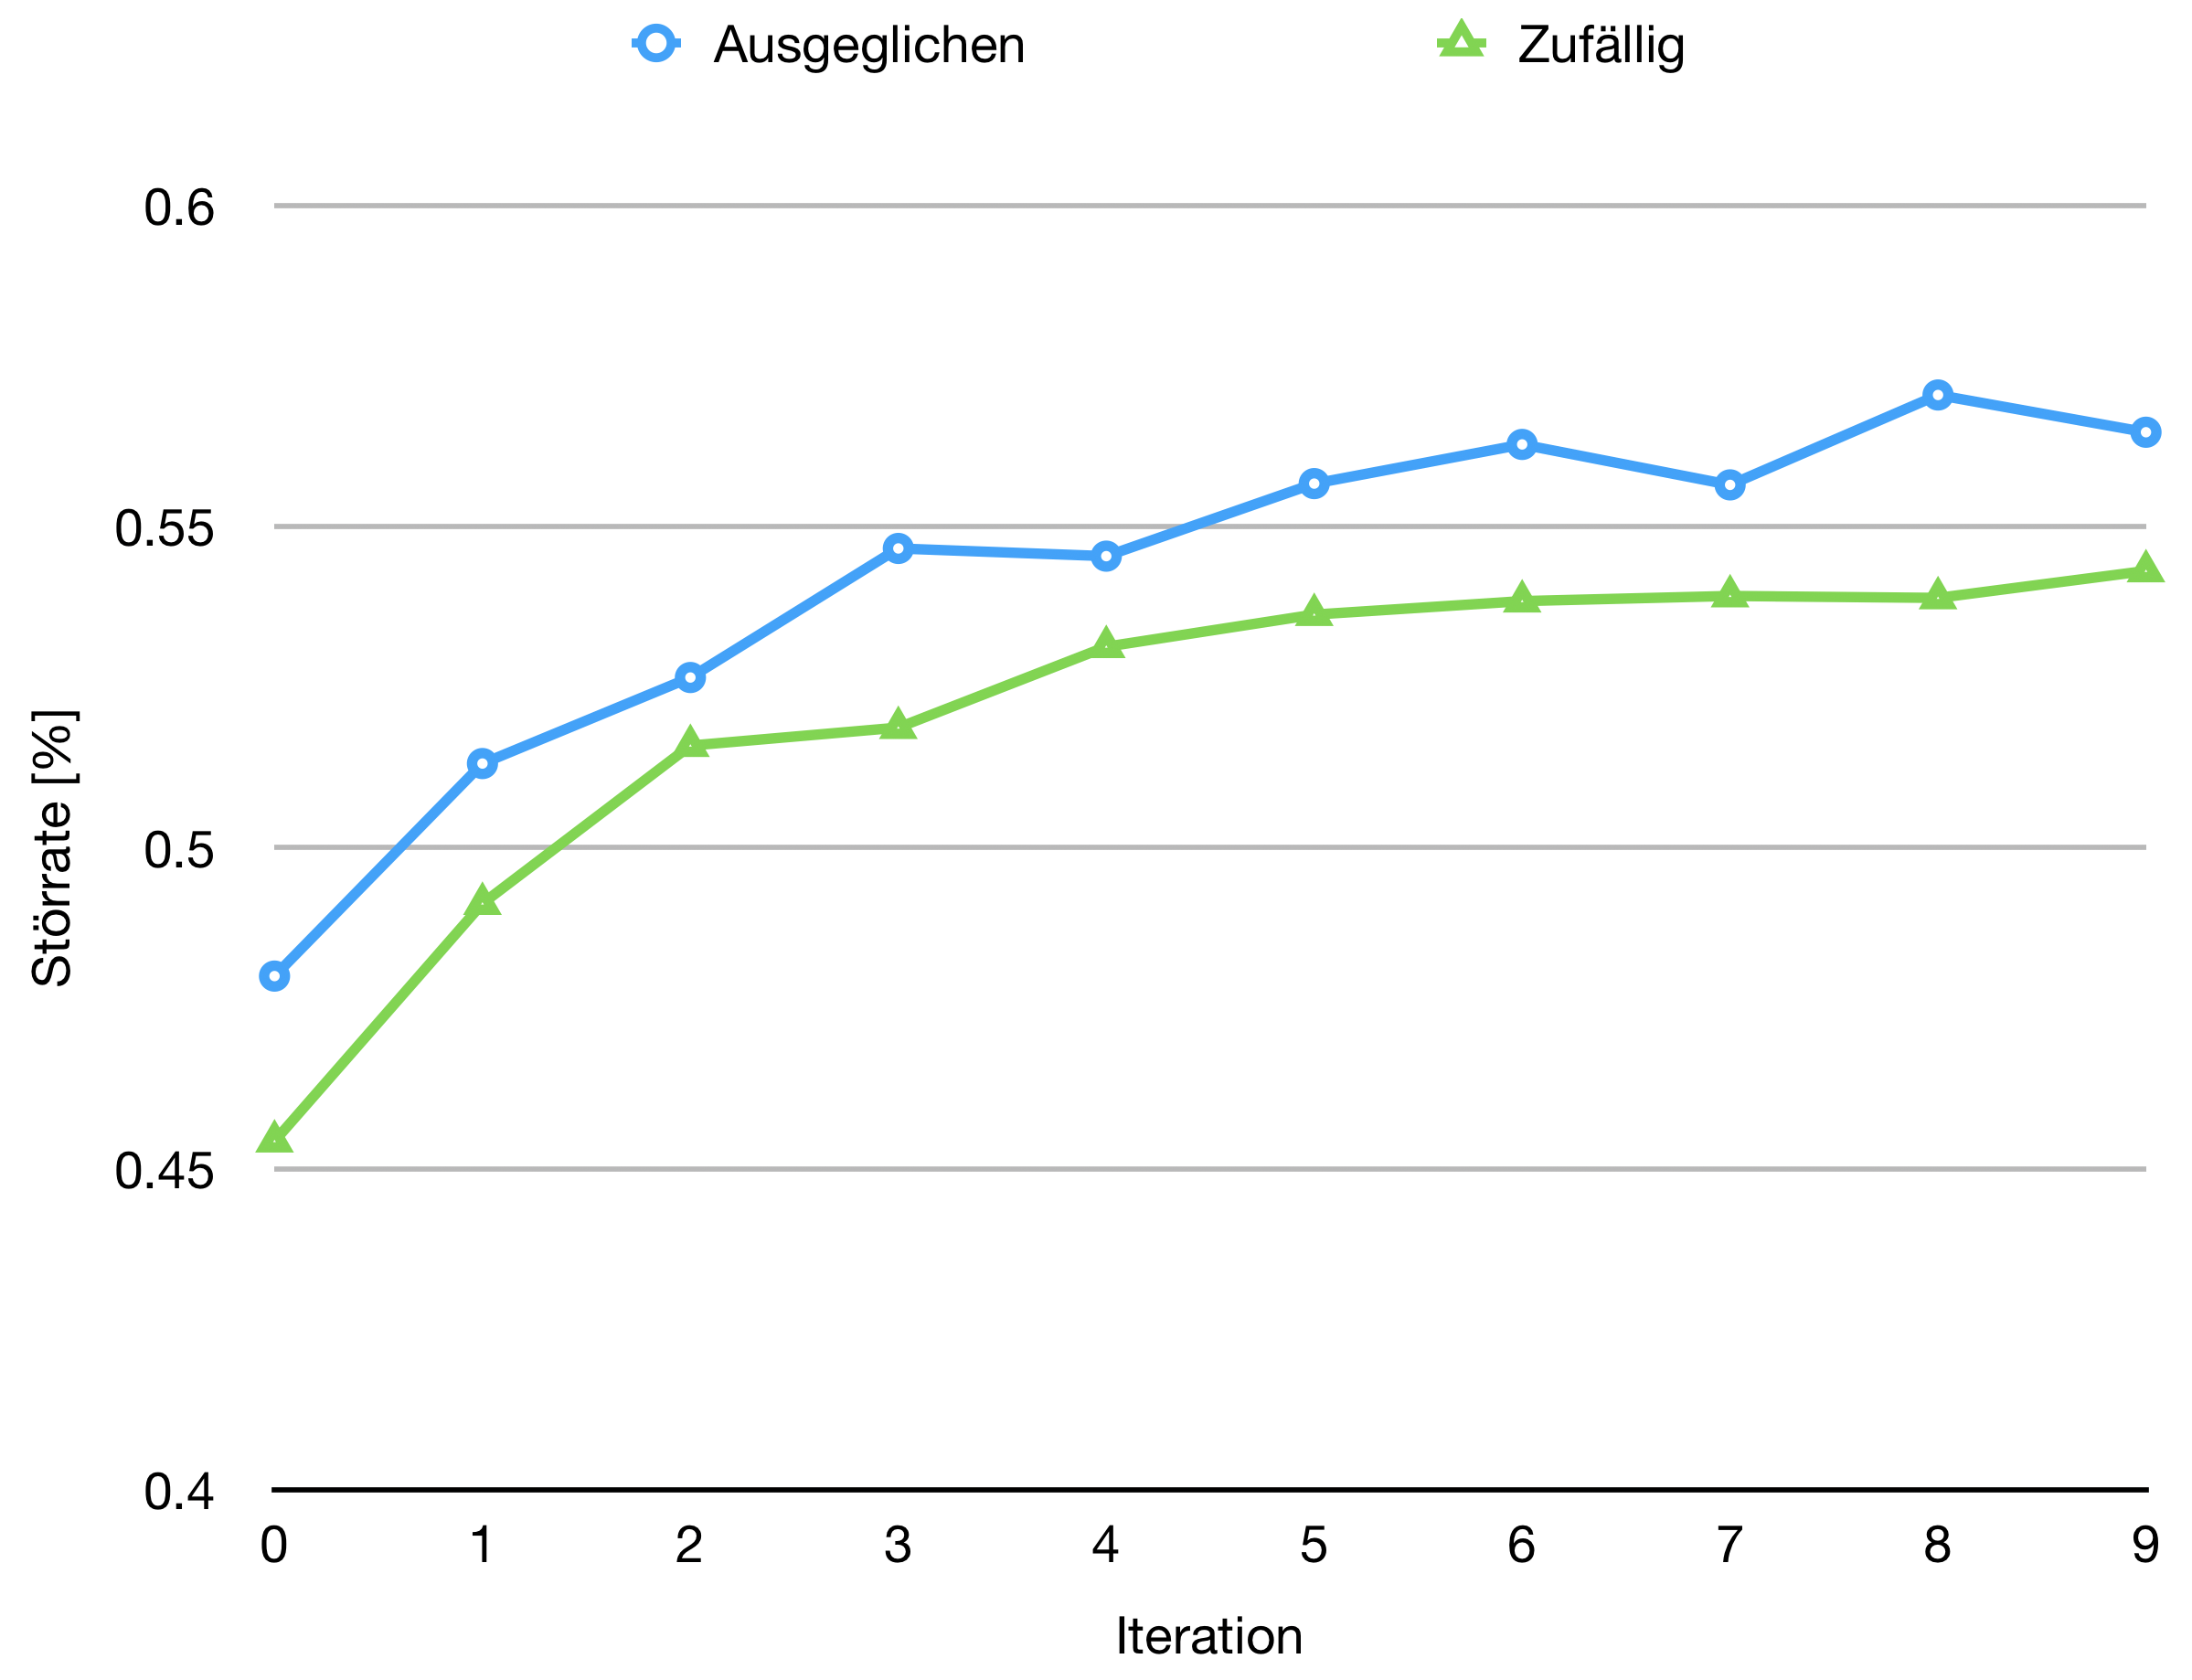
\includegraphics[width=0.7\textwidth]{./images/einfluss_dataset.png}
\label{fig_einfluss_datenset}
\end{figure}


Das Trainingsset wurde zufällig aus dem ImageNet-Trainingsset \cite{russakovsky_imagenet_2015} gewählt. 
Aufgrund der zufällig gewählten Bilder sind einige Klassen nicht oder nur mit wenigen Bildern vertreten. 
Andere Klassen hingegen mit viel mehr Bildern. 
Um diesem Ungleichgewicht entgegenzuwirken, wird ein zweites Datenset erstellt. 
Darin sind von jeder Klasse $10$ Bilder enthalten. 
Die $10$ Bilder pro Klasse werden wiederum zufällig aus dem Trainingsset von ImageNet gewählt. 
Da im ImageNet-Datensatz $1'000$ Klassen enthalten sind, entsteht so wieder ein Datenset, das aus $10'000$ Bildern besteht. 
In diesem Trainingsset sind die Verhältnisse zwischen den Klassen ausgeglichen.

Auf diesem Trainingsset wird ein Störwert für VGG-16 generiert und dessen Störrate auf dem Validation-Set gemessen. 
Mit dem ausgeglichenen Trainingsset wurde in jeder Iteration eine bessere Störrate als mit dem komplett zufälligen Trainingsset erreicht. 
Die Störrate war nach $10$ Iterationen um $2.2\%$ höher, als mit einem zufällig gewählten Trainingsset erreicht wurde. 

Mit einem ausgeglichenen Trainingsset kann die Störrate minimal verbessert werden. 
Die Unterschiede zu den Ergebnissen von Moosavi-Dezfooli et al. können damit aber noch nicht erklärt werden.


\chapter{Resultate Kombinationsverfahren}
\label{c_resultate_optimierung}

Die Kombinationsverfahren werden mit VGG-16 und Inception durchgeführt. 
Die Transferierbarkeit auf ein drittes Modell wird anhand von ResNet-152 gemessen. 
Alle Störwerte wurden in $l_\infty$ mit $\xi=10$ berechnet. 
Als Trainingsset wurden analog der Originalarbeit $10'000$ Bilder verwendet. 
DeepFool wurde mit $\eta=0.02$, $i_d=10$ und einer Anzahl getesteter Klassen von $50$ generiert.


\section{Lineare Interpolation}

\begin{figure}[h]
\caption{Lineare Interpolation von VGG-16-Störwert (links) nach Inception-Störwert (rechts)}
\centering
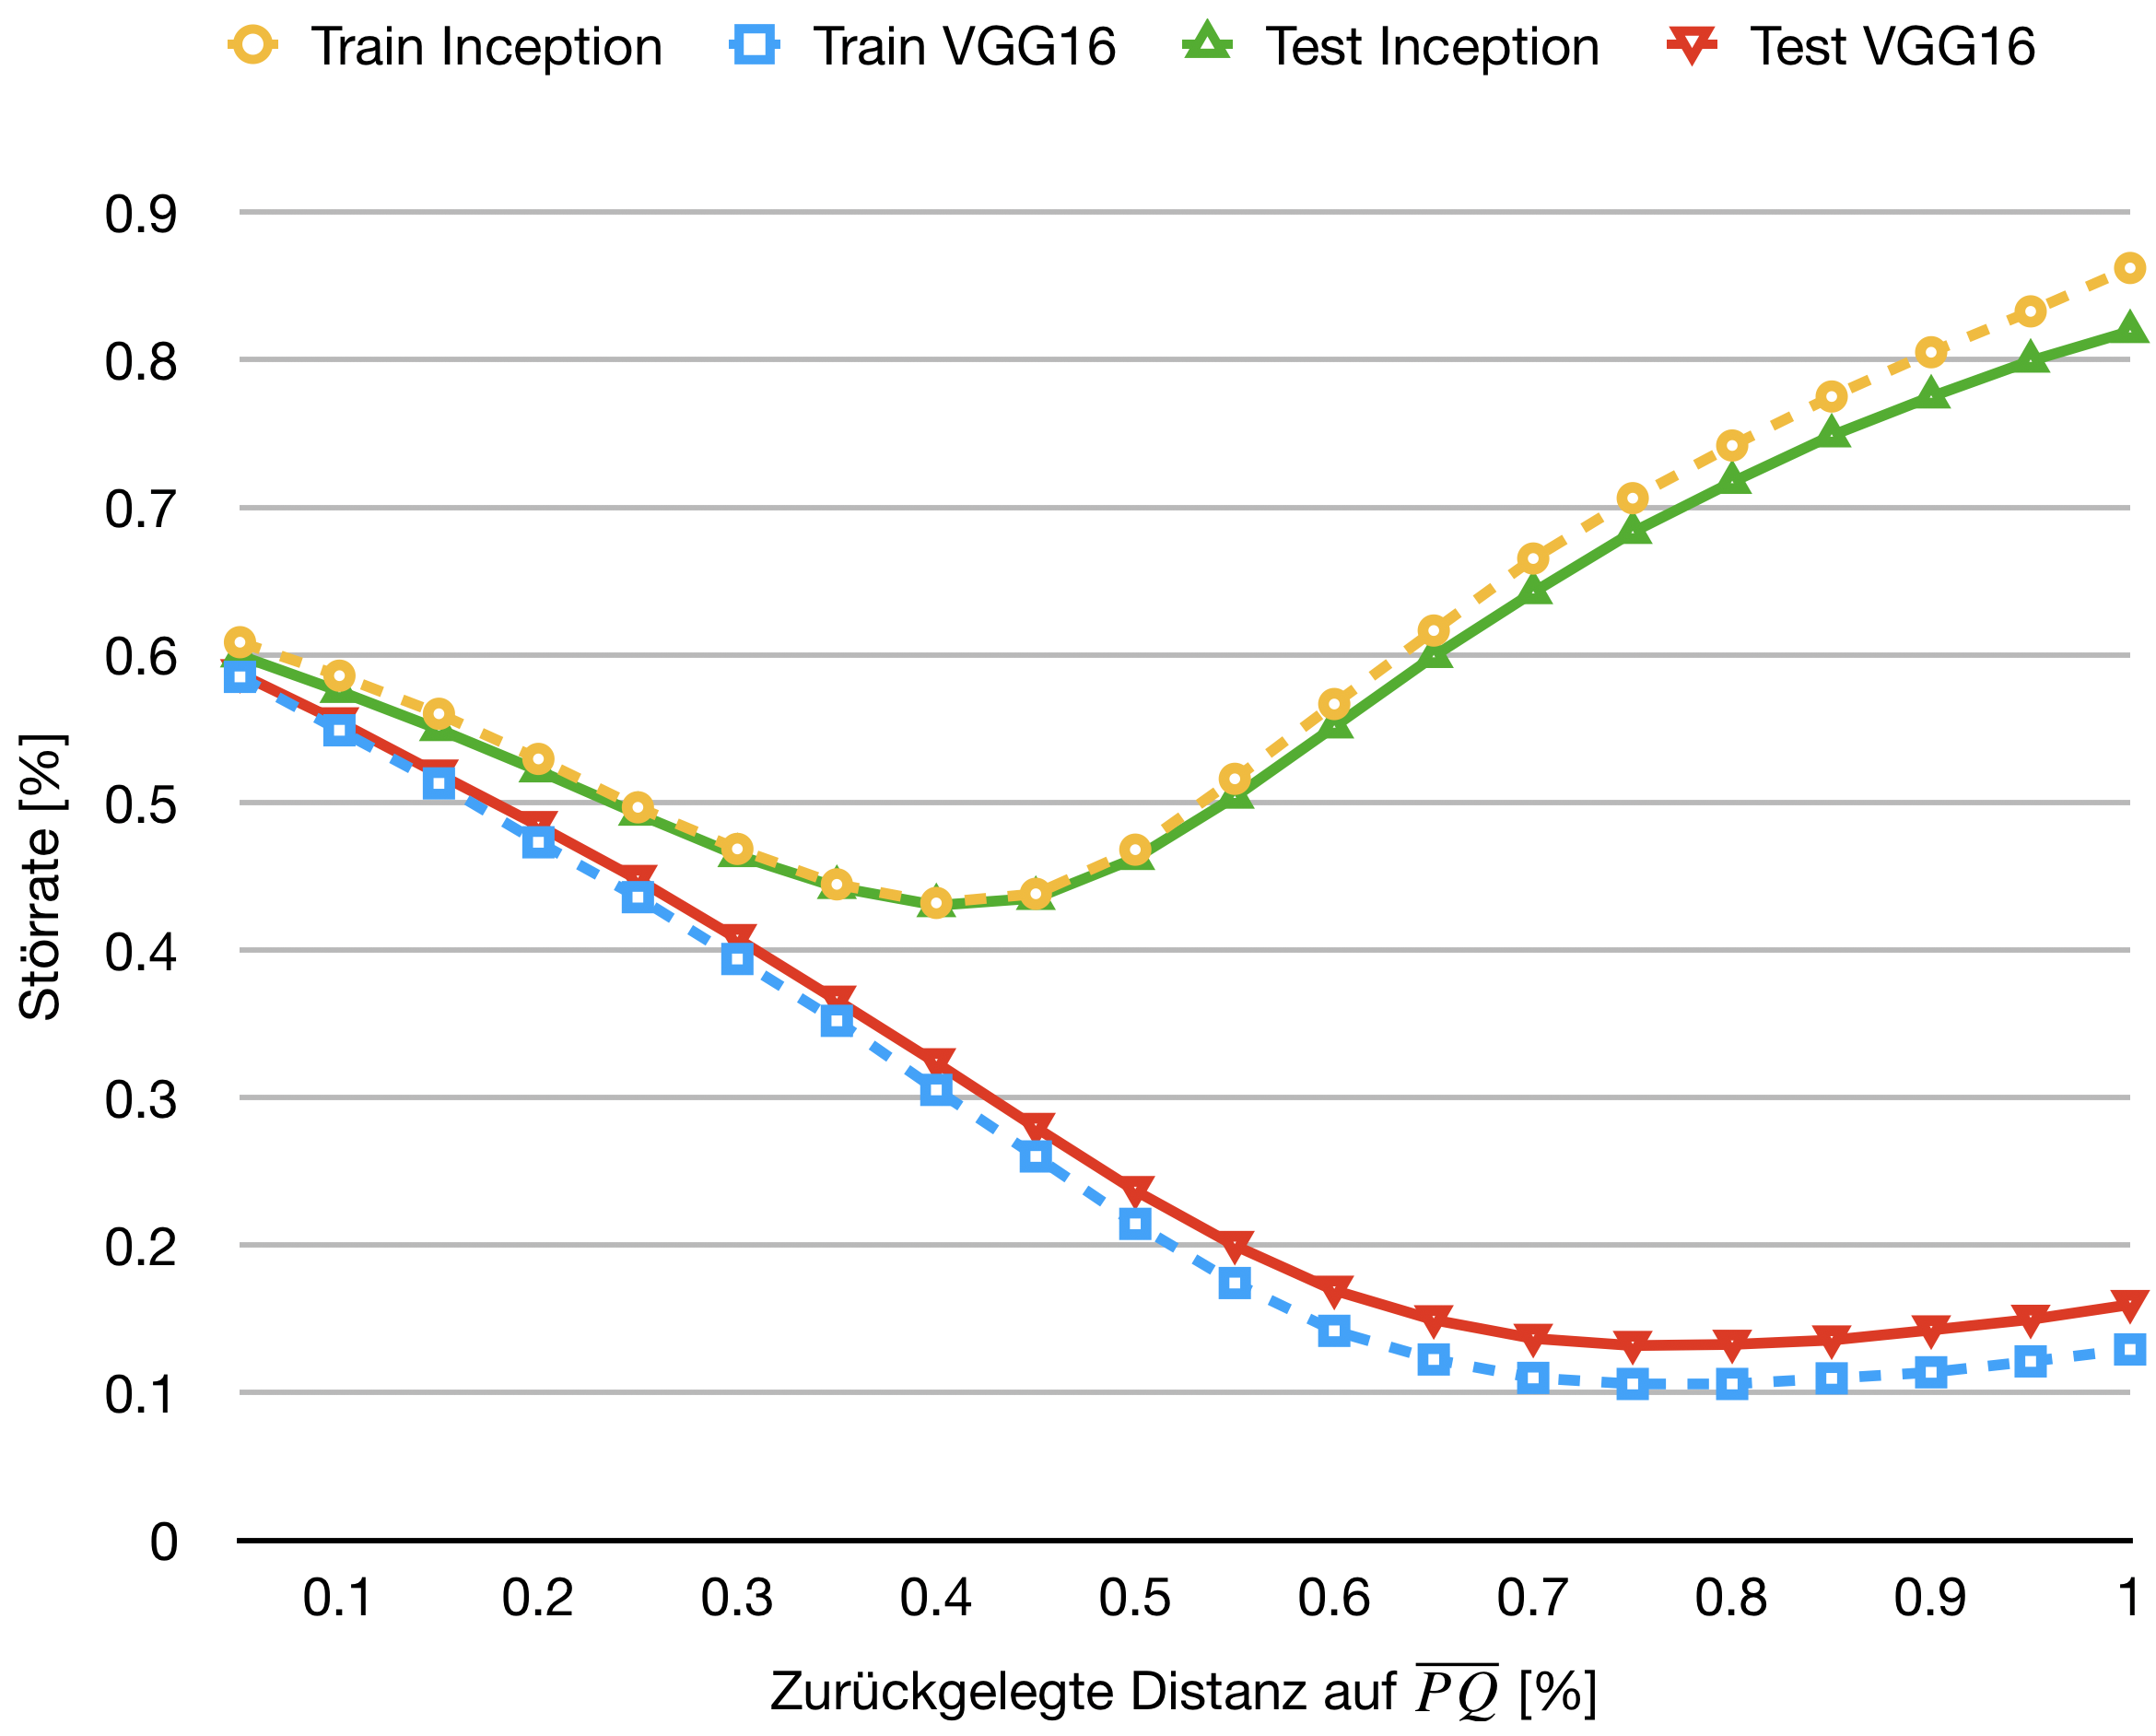
\includegraphics[width=0.6\textwidth]{./images/stoerrate_interpolate.png}
\label{fig_stoerrate_interpolate}
\end{figure}

Die Punkte $P$ und $Q$ sind für VGG-16 und Inception berechnete Störwerte. Die Störwerte wurden über $20$ Iterationen auf dem jeweiligen Modell generiert. Die damit erreichten Störraten entsprechen denen aus Tabelle \ref{tbl_stoerraten_reprod_kreuz_linf}.
 
Aus der Strecke von $P$ (Störwert VGG-16) nach $Q$ (Störwert Inception) wurden $20$ gleichmässig verteilte Punkte gewählt. 
Die Störrate jedes Punktes wurde auf den beiden Modellen überprüft.

In Abbildung \ref{fig_stoerrate_interpolate} sind die Störraten der Punkte pro Modell und Datensatz visualisiert. 
Die Störraten verändern sich nicht linear. 
Die Störrate auf Inception sinkt bis auf $43.2\%$, bevor sie wieder auf die Störrate von $Q$ ansteigt. 
Das gleiche Verhalten ist bei VGG-16 sichtbar, dessen Störrate auf $10.6\%$ absinkt. 
Die minimale erreichte Störrate ist für VGG-16 näher am Inception-Störwert und für Inception ist sie näher am VGG-16-Störwert. 
Kein Störwert aus $\overline{PQ}$ war besser als die Ausgangswerte selbst, die lineare Interpolation zweier Störwerte bildet keine besseren Störraten als einzeln generierte Störwerte.

\section{Finetuning auf Modell}

\begin{figure}[h]
\caption{Störraten eines mit Finetuning optimierten Störwertes}
\centering
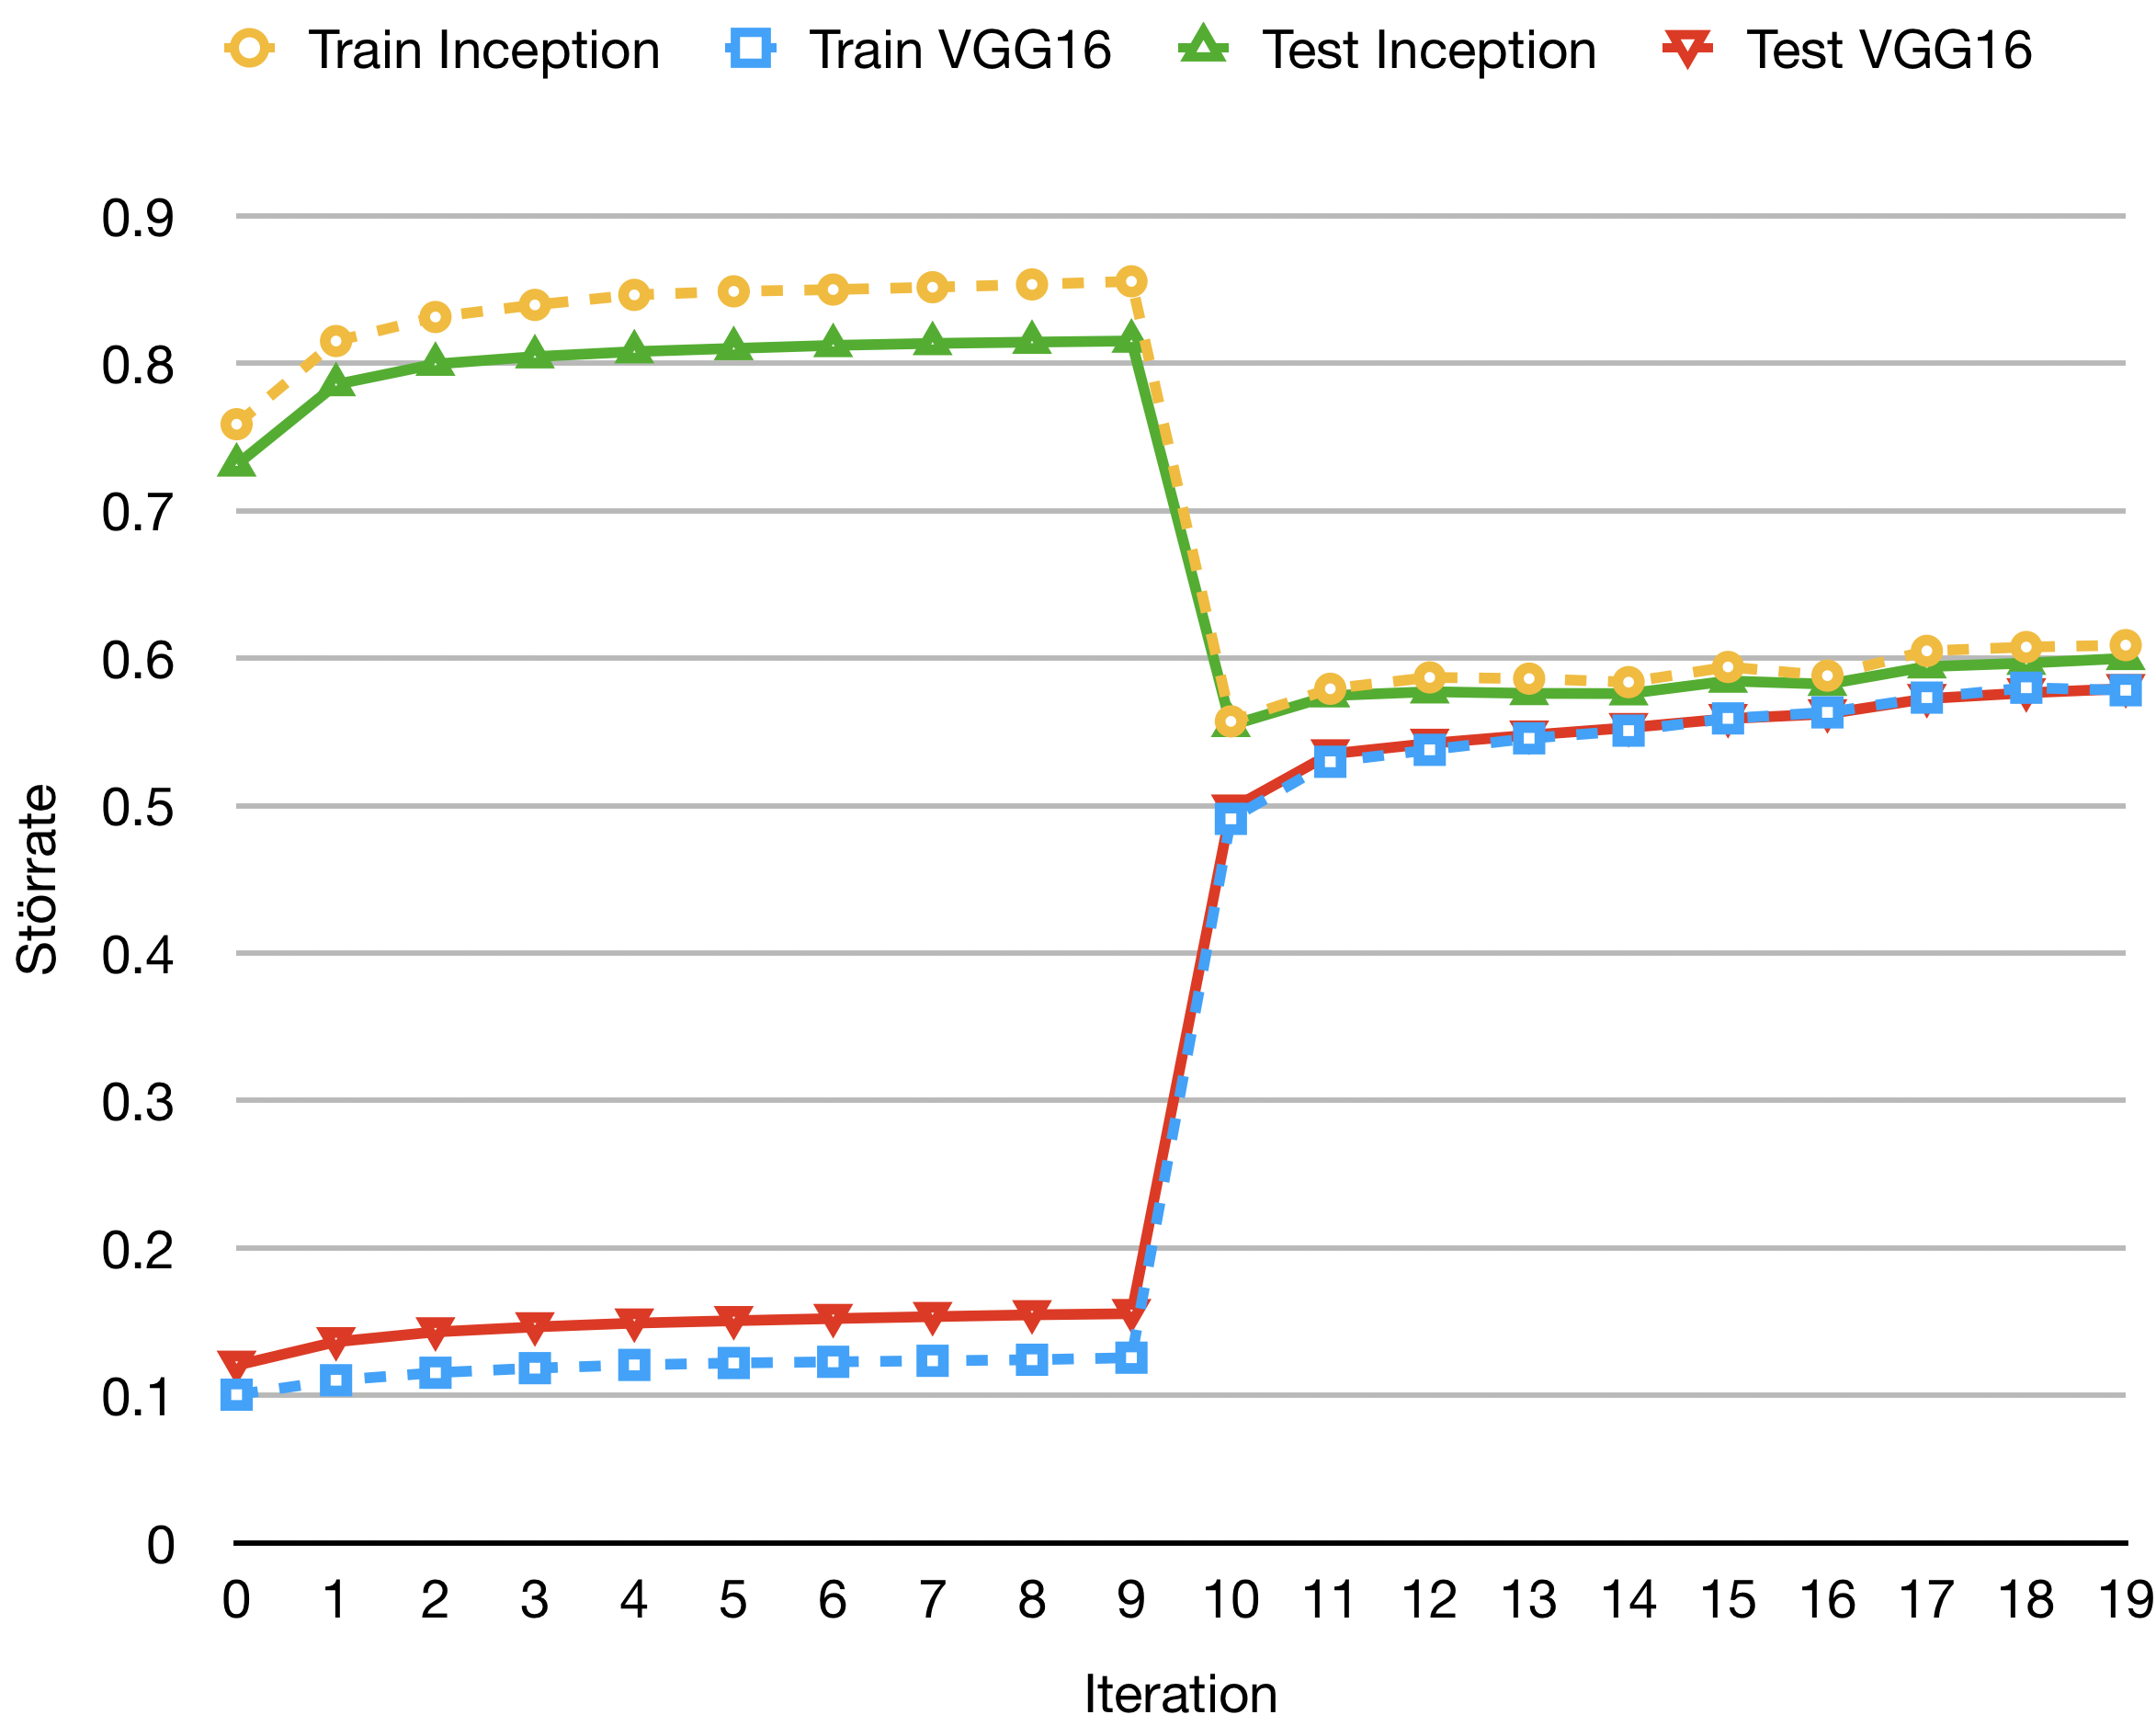
\includegraphics[width=0.6\textwidth]{./images/stoerrate_finetuning.png}
\label{fig_stoerrate_finetuning}
\end{figure}


\begin{figure}[h]
\caption{Finetuning auf anderem Modell, Initialmodell Inception, Finetuning auf VGG-16}
\centering
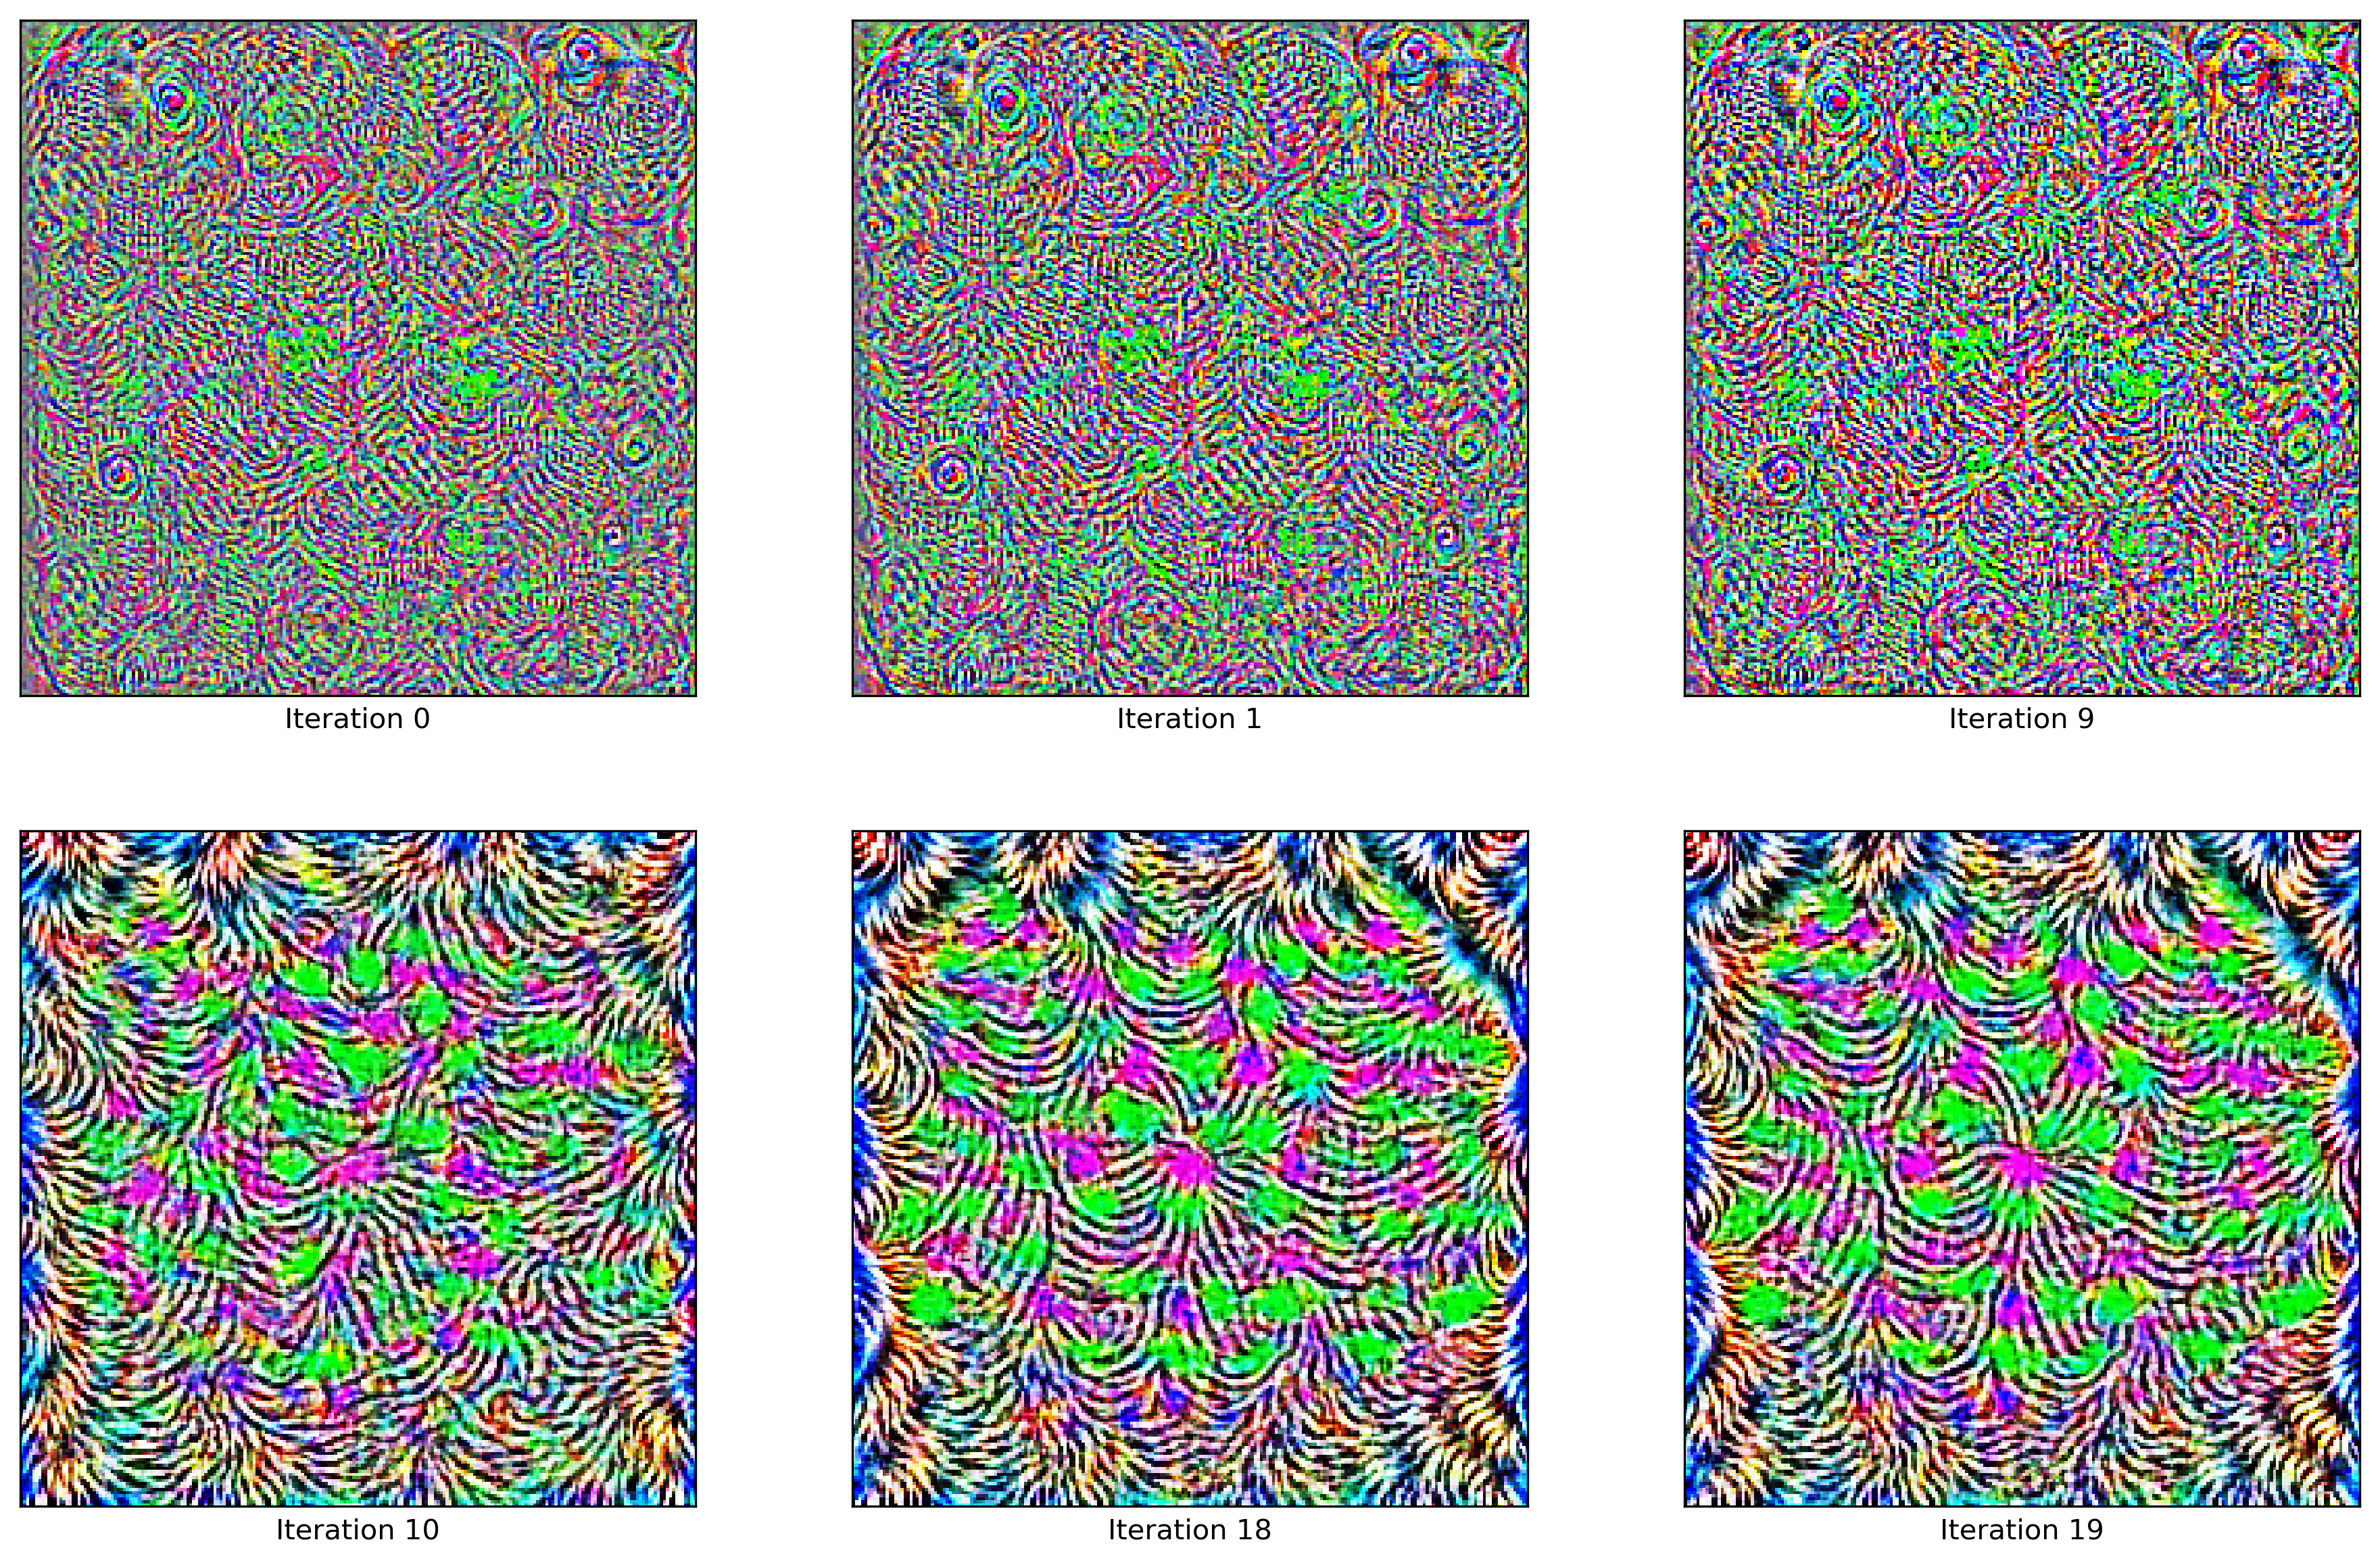
\includegraphics[width=\textwidth]{./images/comb1_inception_vgg16.png} 
\label{fig_stoerwerte_finetuning}
\end{figure}


Der Störwert wird zuerst für $10$ Iterationen nur auf Inception generiert (Abbildung \ref{fig_stoerrate_finetuning}, Iterationen $0$ bis und mit $9$).  
Anschliessend wird für weitere $10$ Iterationen auf VGG-16 trainiert (Iterationen $10$ bis und mit $19$). 
Bereits nach einer Iteration auf VGG-16 verbessert sich die Störrate auf VGG-16 um $36.5\%$, die Störrate für Inception sinkt dabei um $29.8\%$. 
Der nach insgesamt $20$ Iterationen errechnete Störwert erreicht auf dem Validation-Set für Inception eine Störrate von $59.9\%$ und für VGG-16 $57.9\%$.

Mit jeder weiteren Iteration verbessert sich die Störrate auf dem VGG-16-Modell. 
Beachtenswert ist hier, dass die Störrate für Inception ebenfalls wieder ansteigt, obwohl dieses Modell für das Generieren des Störwertes nicht weiter verwendet wird (siehe Abbildung \ref{fig_stoerrate_finetuning}). 

In Abbildung \ref{fig_stoerwerte_finetuning} sind einige Störwerte des Finetunings visualisiert. 
Der Störwert nimmt bereits eine Iteration nach Modellwechsel die Struktur des neuen Modells an (Iteration $10$).
Der errechnete Störwert entspricht visuell einem Störwert, der nur auf VGG-16 errechnet wurde (siehe Abbildung \ref{fig_stoerwerte}).

Obwohl der Störwert also visuell einem VGG-16-Störwert entspricht und auf diesem weiter generiert wird, steigt auch die Störrate für das Inception-Modell weiter an. Der nach $20$ Iterationen generierte Störwert erzielt auf Inception und VGG-16 ähnliche Störraten wie ein nur mit VGG-16 generierter Störwert. Es scheinen also nur wenige oder keine Informationen aus dem vorhergehenden Inception-Störwert beibehalten zu bleiben.

\section{Abwechselndes Training}

\begin{figure}[h]
\caption{Störraten eines abwechselnd generierten Störwertes}
\centering
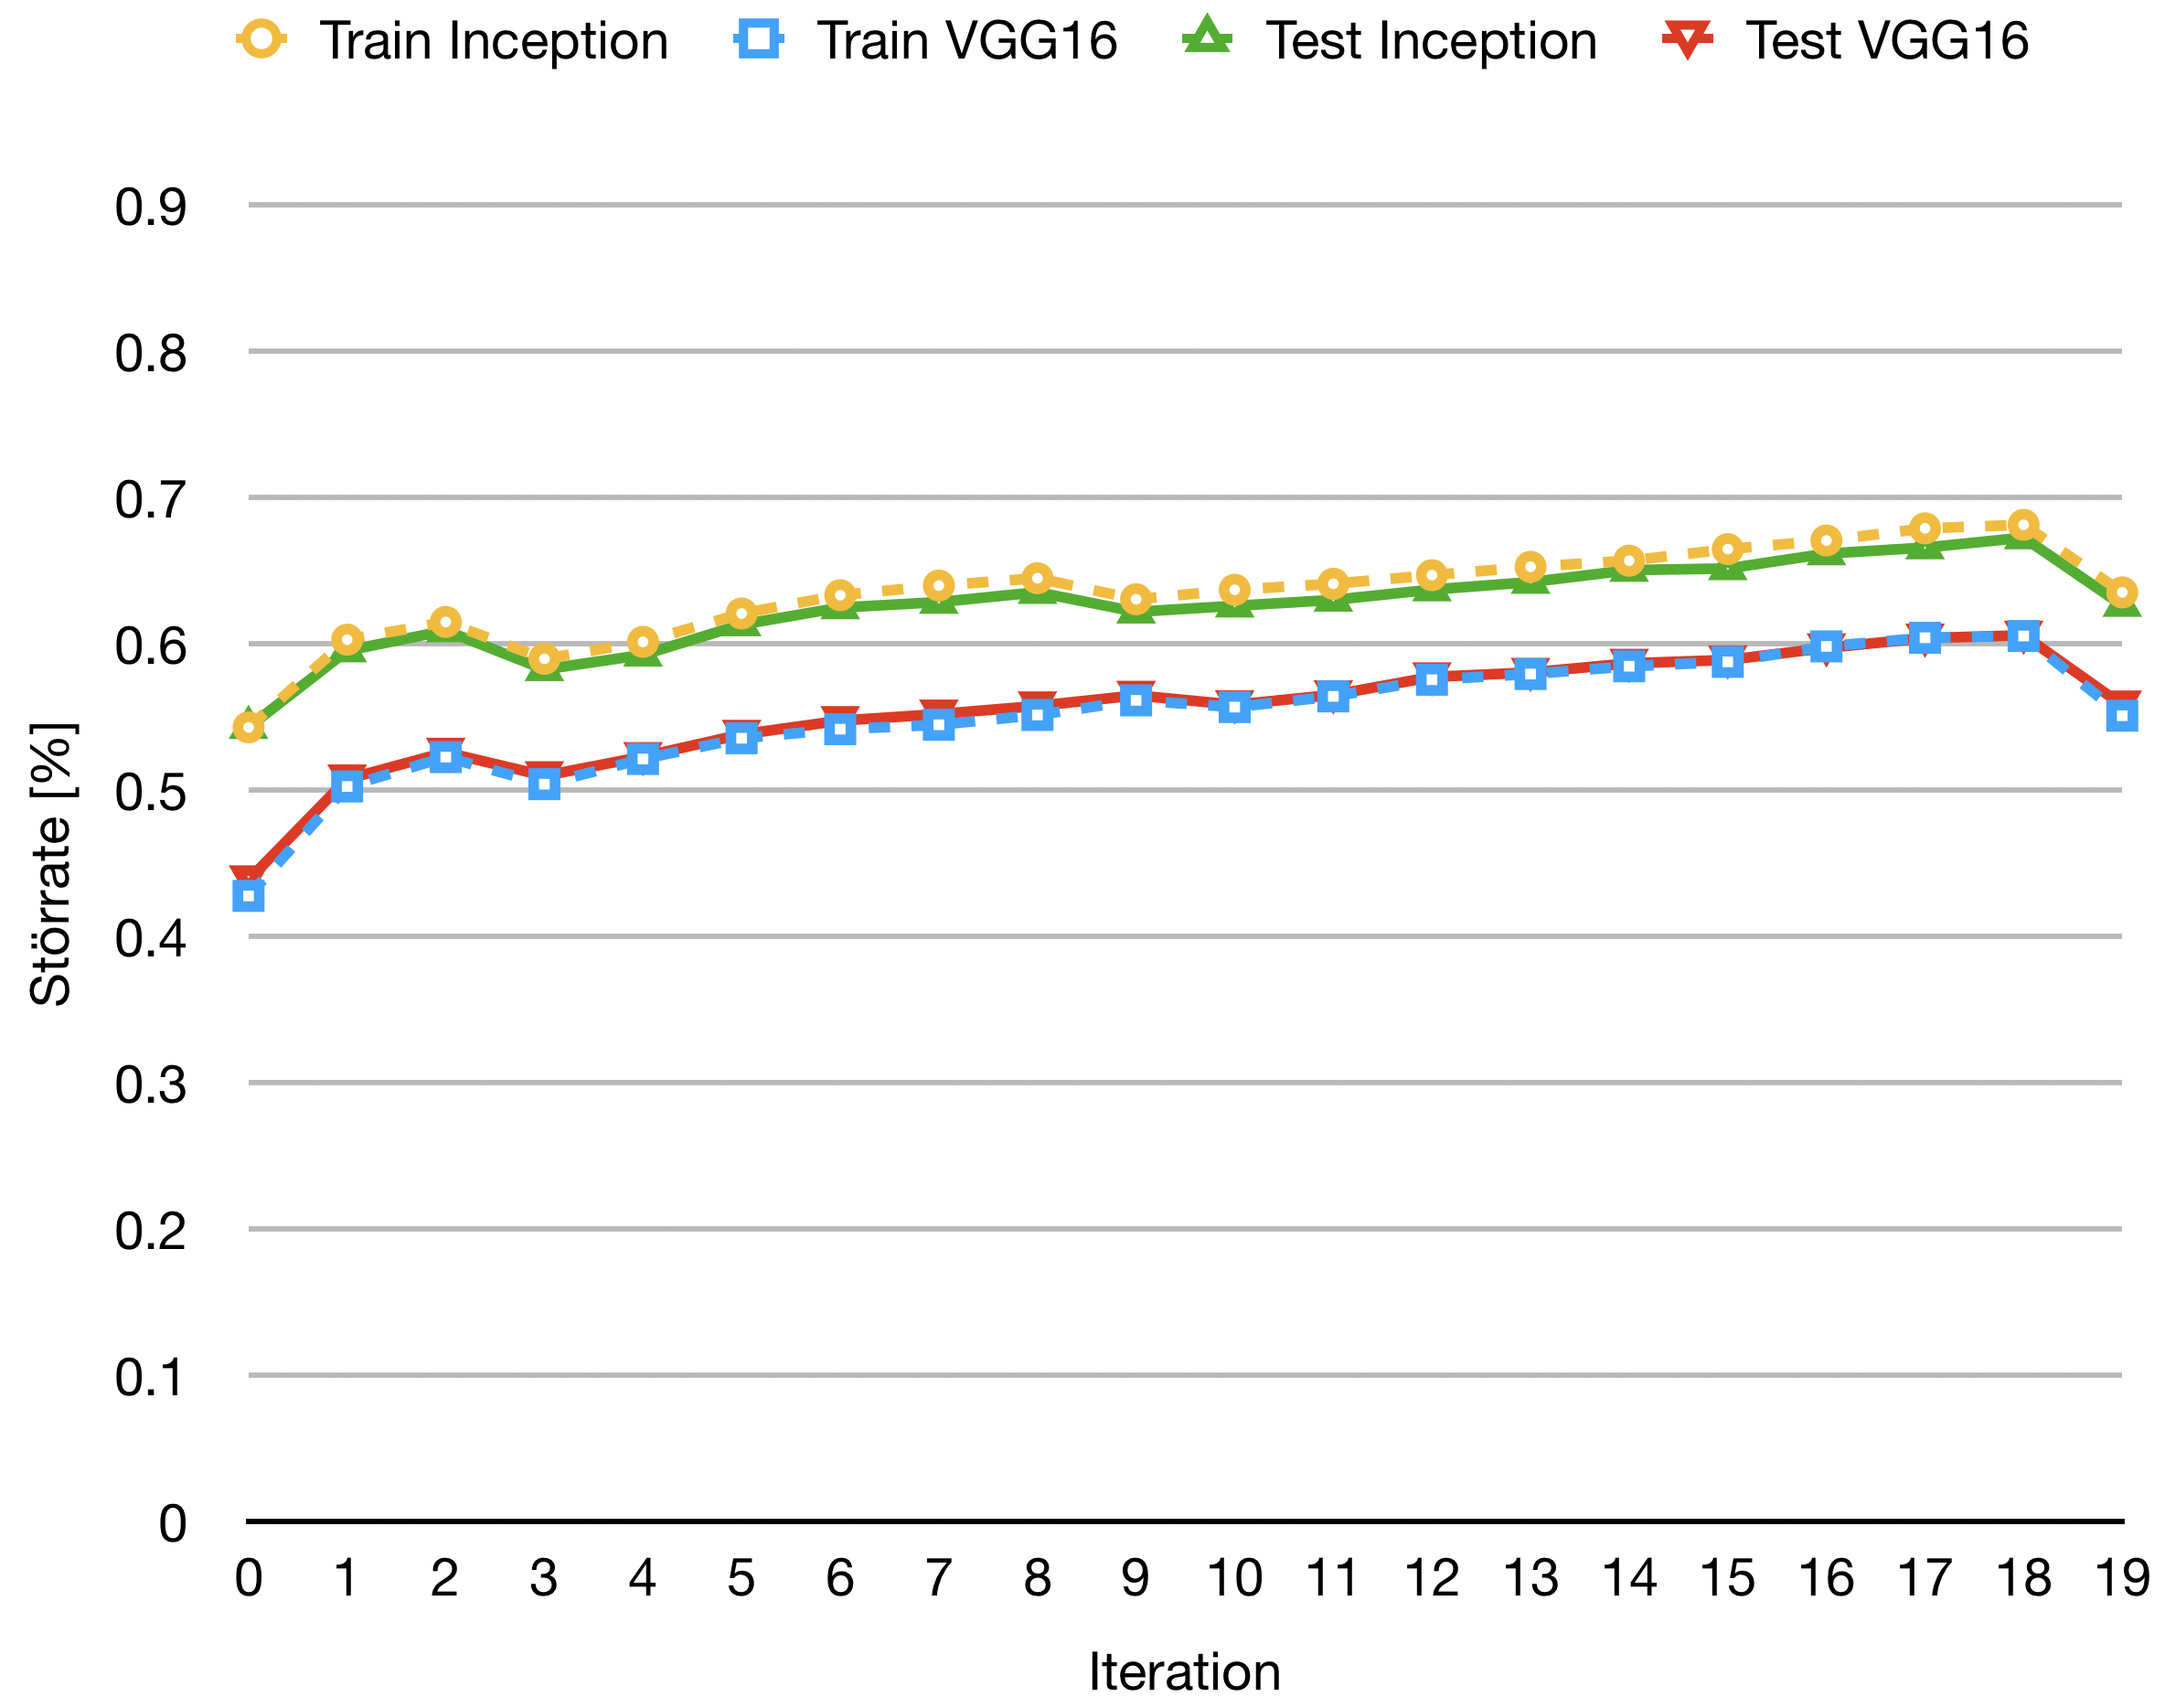
\includegraphics[width=0.6\textwidth]{./images/stoerrate_alternate.png}
\label{fig_stoerrate_alternate}
\end{figure}


\begin{figure}[h]
\caption{Abwechselndes Generieren auf Inception und VGG-16}
\centering
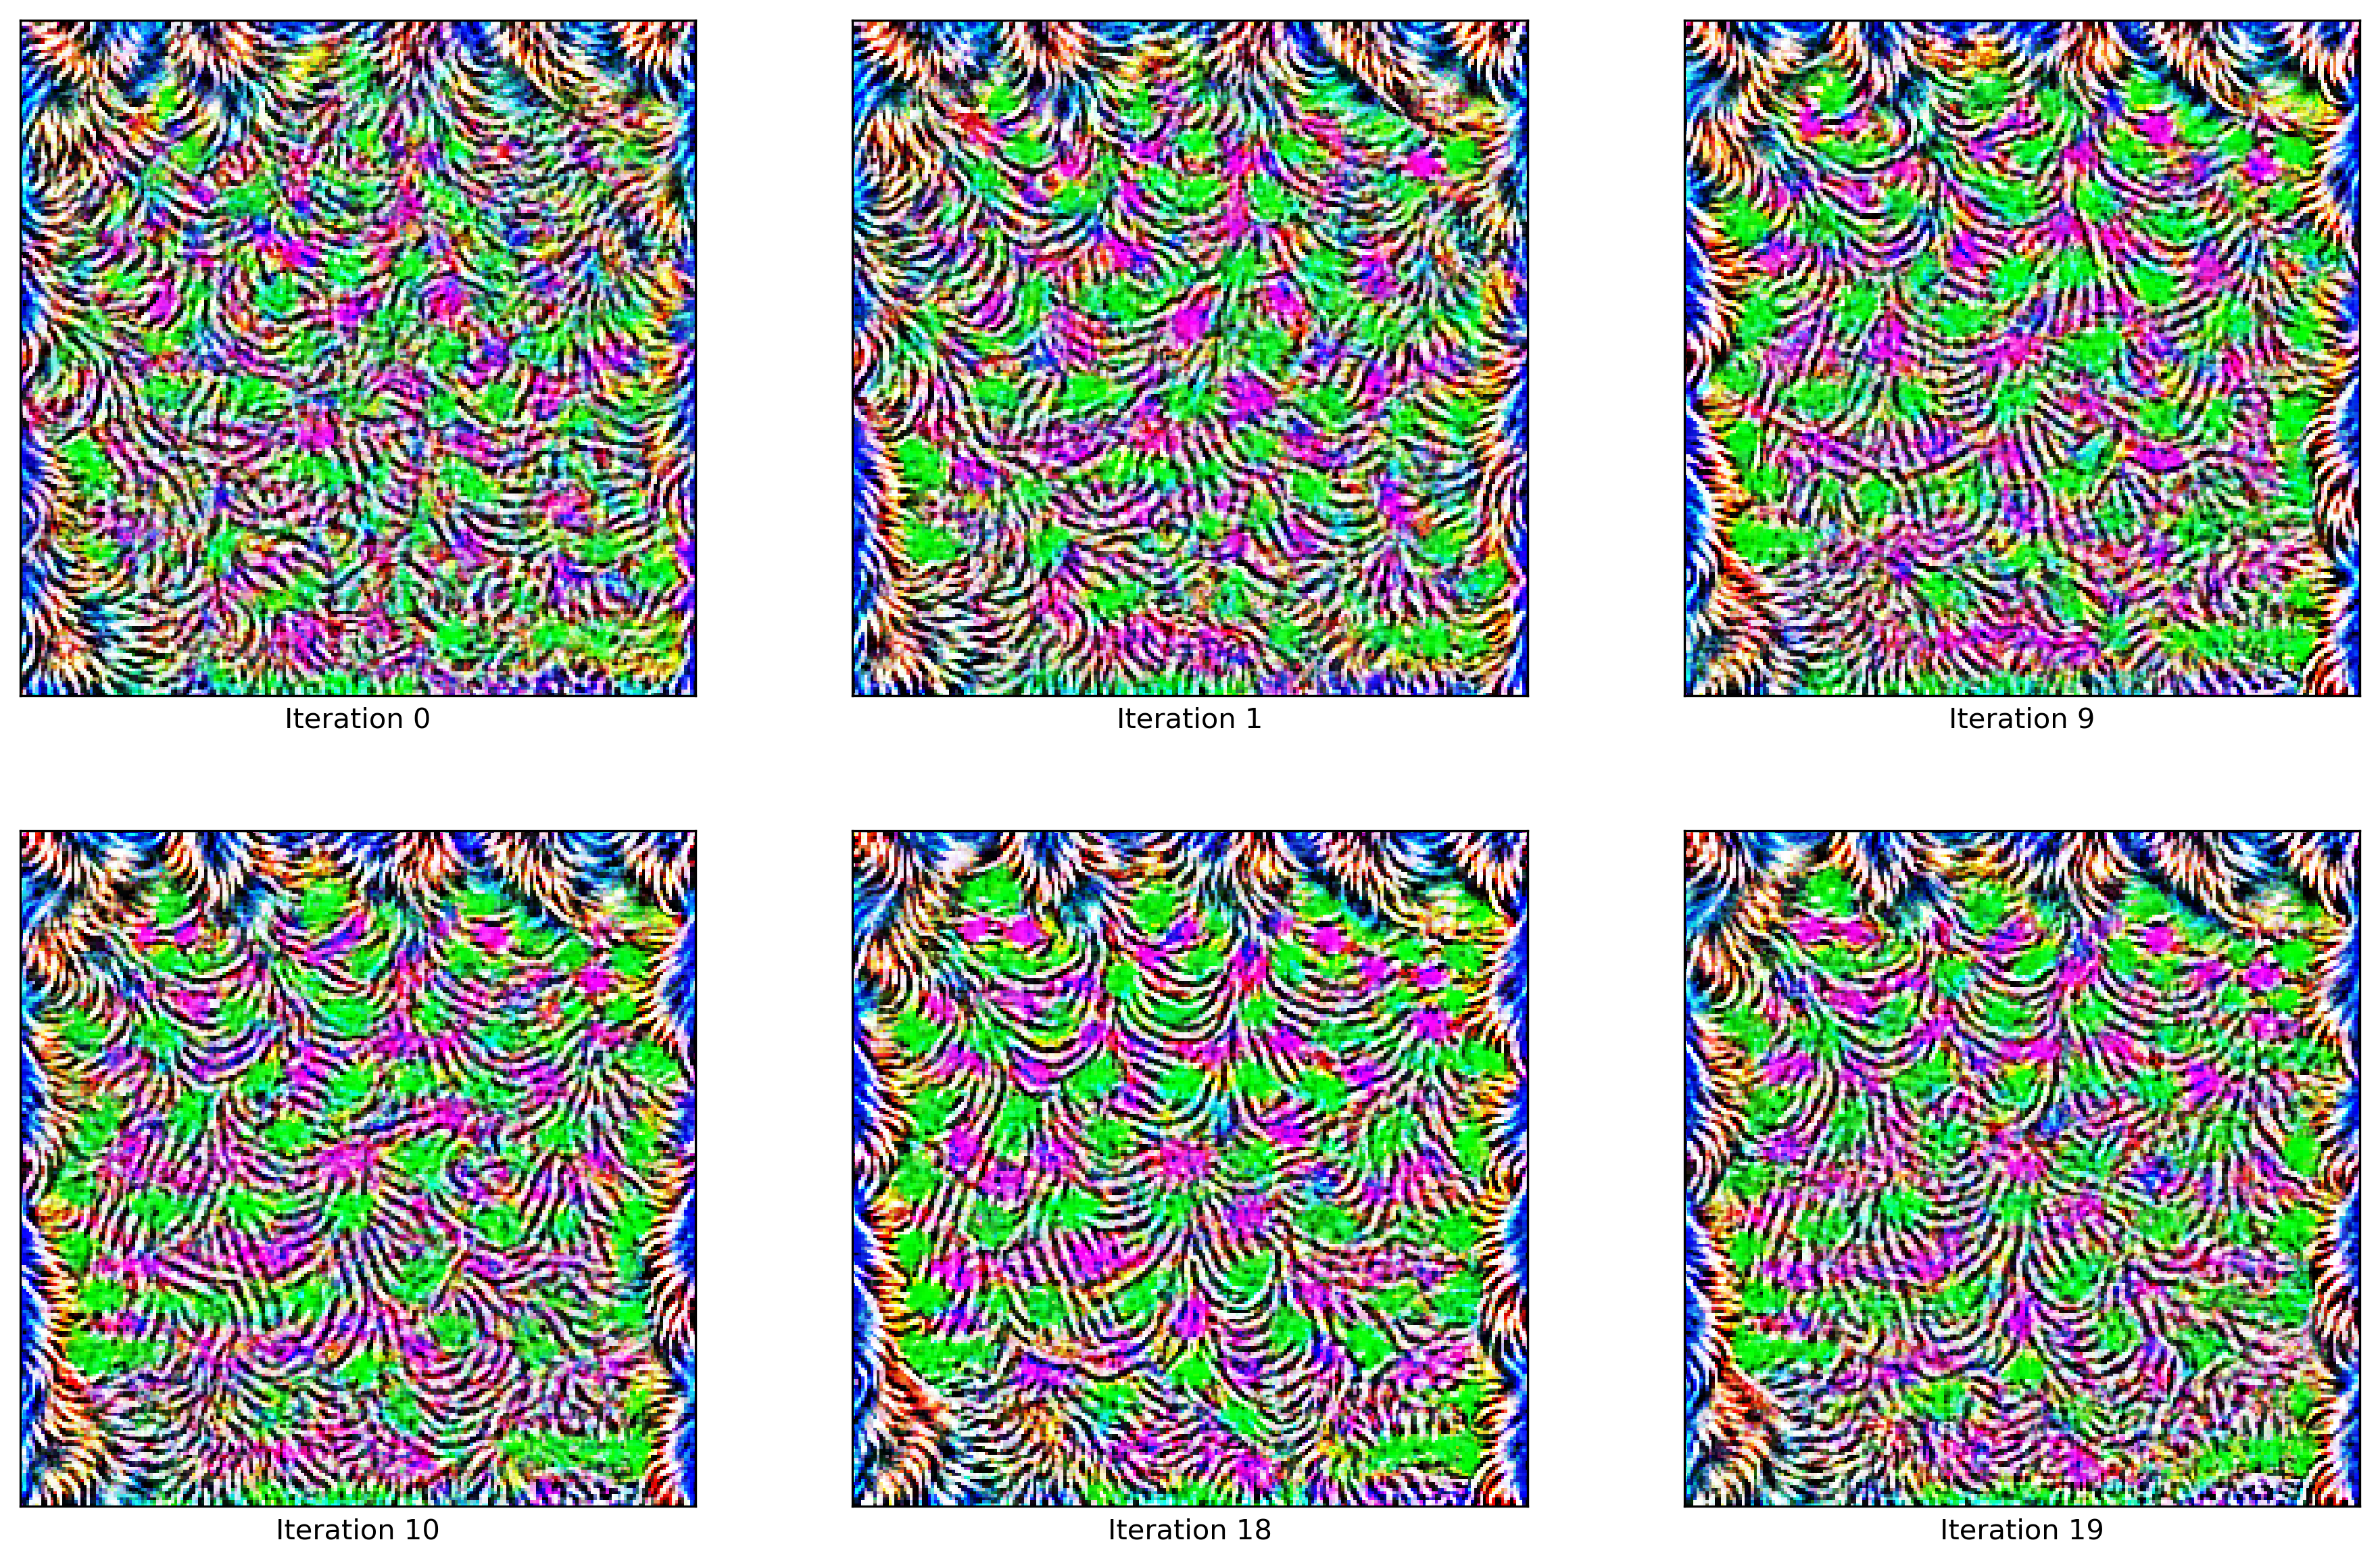
\includegraphics[width=\textwidth]{./images/comb2_inception_vgg16.png}
\label{fig_stoerwerte_alternate}
\end{figure}


Der Störwert wird abwechselnd auf Inception und VGG-16 generiert. 
Das verwendete Modell wird nach jedem Bild abgewechselt. 
Die Störrate ist nach einer Iteration für Inception bei $54.3\%$ und für VGG-16 bei $43.9\%$. 
Nach weiteren Iterationen wird die Störrate für beide Modelle zunehmend besser.

Die besten Störraten auf dem Validation-Set wurden nach $19$ Iterationen gemessen. 
Inception wurde in dieser Iteration zu $67.3\%$ und VGG-16 zu $60.6\%$ gestört (siehe Abbildung \ref{fig_stoerrate_alternate}).
Bei einem visuellen Vergleich wird sichtbar, dass der generierte Störwert eine ähnliche Struktur annimmt, wie ein rein auf VGG-16 generierter Störwert (siehe Abbildung \ref{fig_stoerwerte_alternate}). Eine ähnliche Struktur macht insofern Sinn, da ein rein auf VGG-16 generierter Störwert bereits auf beiden Modellen eine hohe Störrate erzielt.

Die mit dieser Kombination generierten Störwerte stören VGG-16 um $1.9\%$ stärker, als ein rein auf VGG-16 generierter Störwert. Durch das Abwechseln der Modelle scheint der Störwert nicht sofort in ein lokales Minimum zu fallen, in dem er VGG-16 nicht mehr besser stören kann. 


    
\section{DeepFool für mehrere Modelle}

Die in Abschnitt \ref{c_multifool} beschriebenen Änderungen an DeepFool wurden mit VGG-16 und Inception getestet. Die Kombination erreichte auf beiden Modellen geringere Störraten als mit dem unveränderten DeepFool-Verfahren. Auf einem nicht zum Generieren verwendeten Modell (ResNet-152) ist die Störrate ebenfalls tiefer.

Visuell hat der Störwert am ehesten Ähnlichkeiten mit dem Inception-Störwert. Im Gegensatz zum Inception-Störwert enthält er weniger Struktur und gleicht mehr zufällig verteilten Werten (siehe Abbildung \ref{fig_stoerwerte_multifool}). 

Eine mögliche Erklärung für die schlechten Störraten dieses Verfahrens wäre die Wahl des Klassengrenzen-Paars. Die getestete Implementation sucht die beiden Klassengrenzen mit der kleinsten Distanz zum Bild, beachtet aber die Richtung nicht, in welche gestört werden muss. Wenn die Klassengrenzen einander entgegengesetzt sind, heben sie sich gegenseitig auf oder zeigen in eine Richtung, die sich keiner der beiden Klassengrenzen annähert.



\begin{figure}[h]
\caption{links: Mit angepasstem DeepFool-Verfahren generierter Störwert (nach $20$ Iterationen). Rechts: Störraten auf VGG-16 und Inception auf Trainings- und Validation-Set.}
\centering
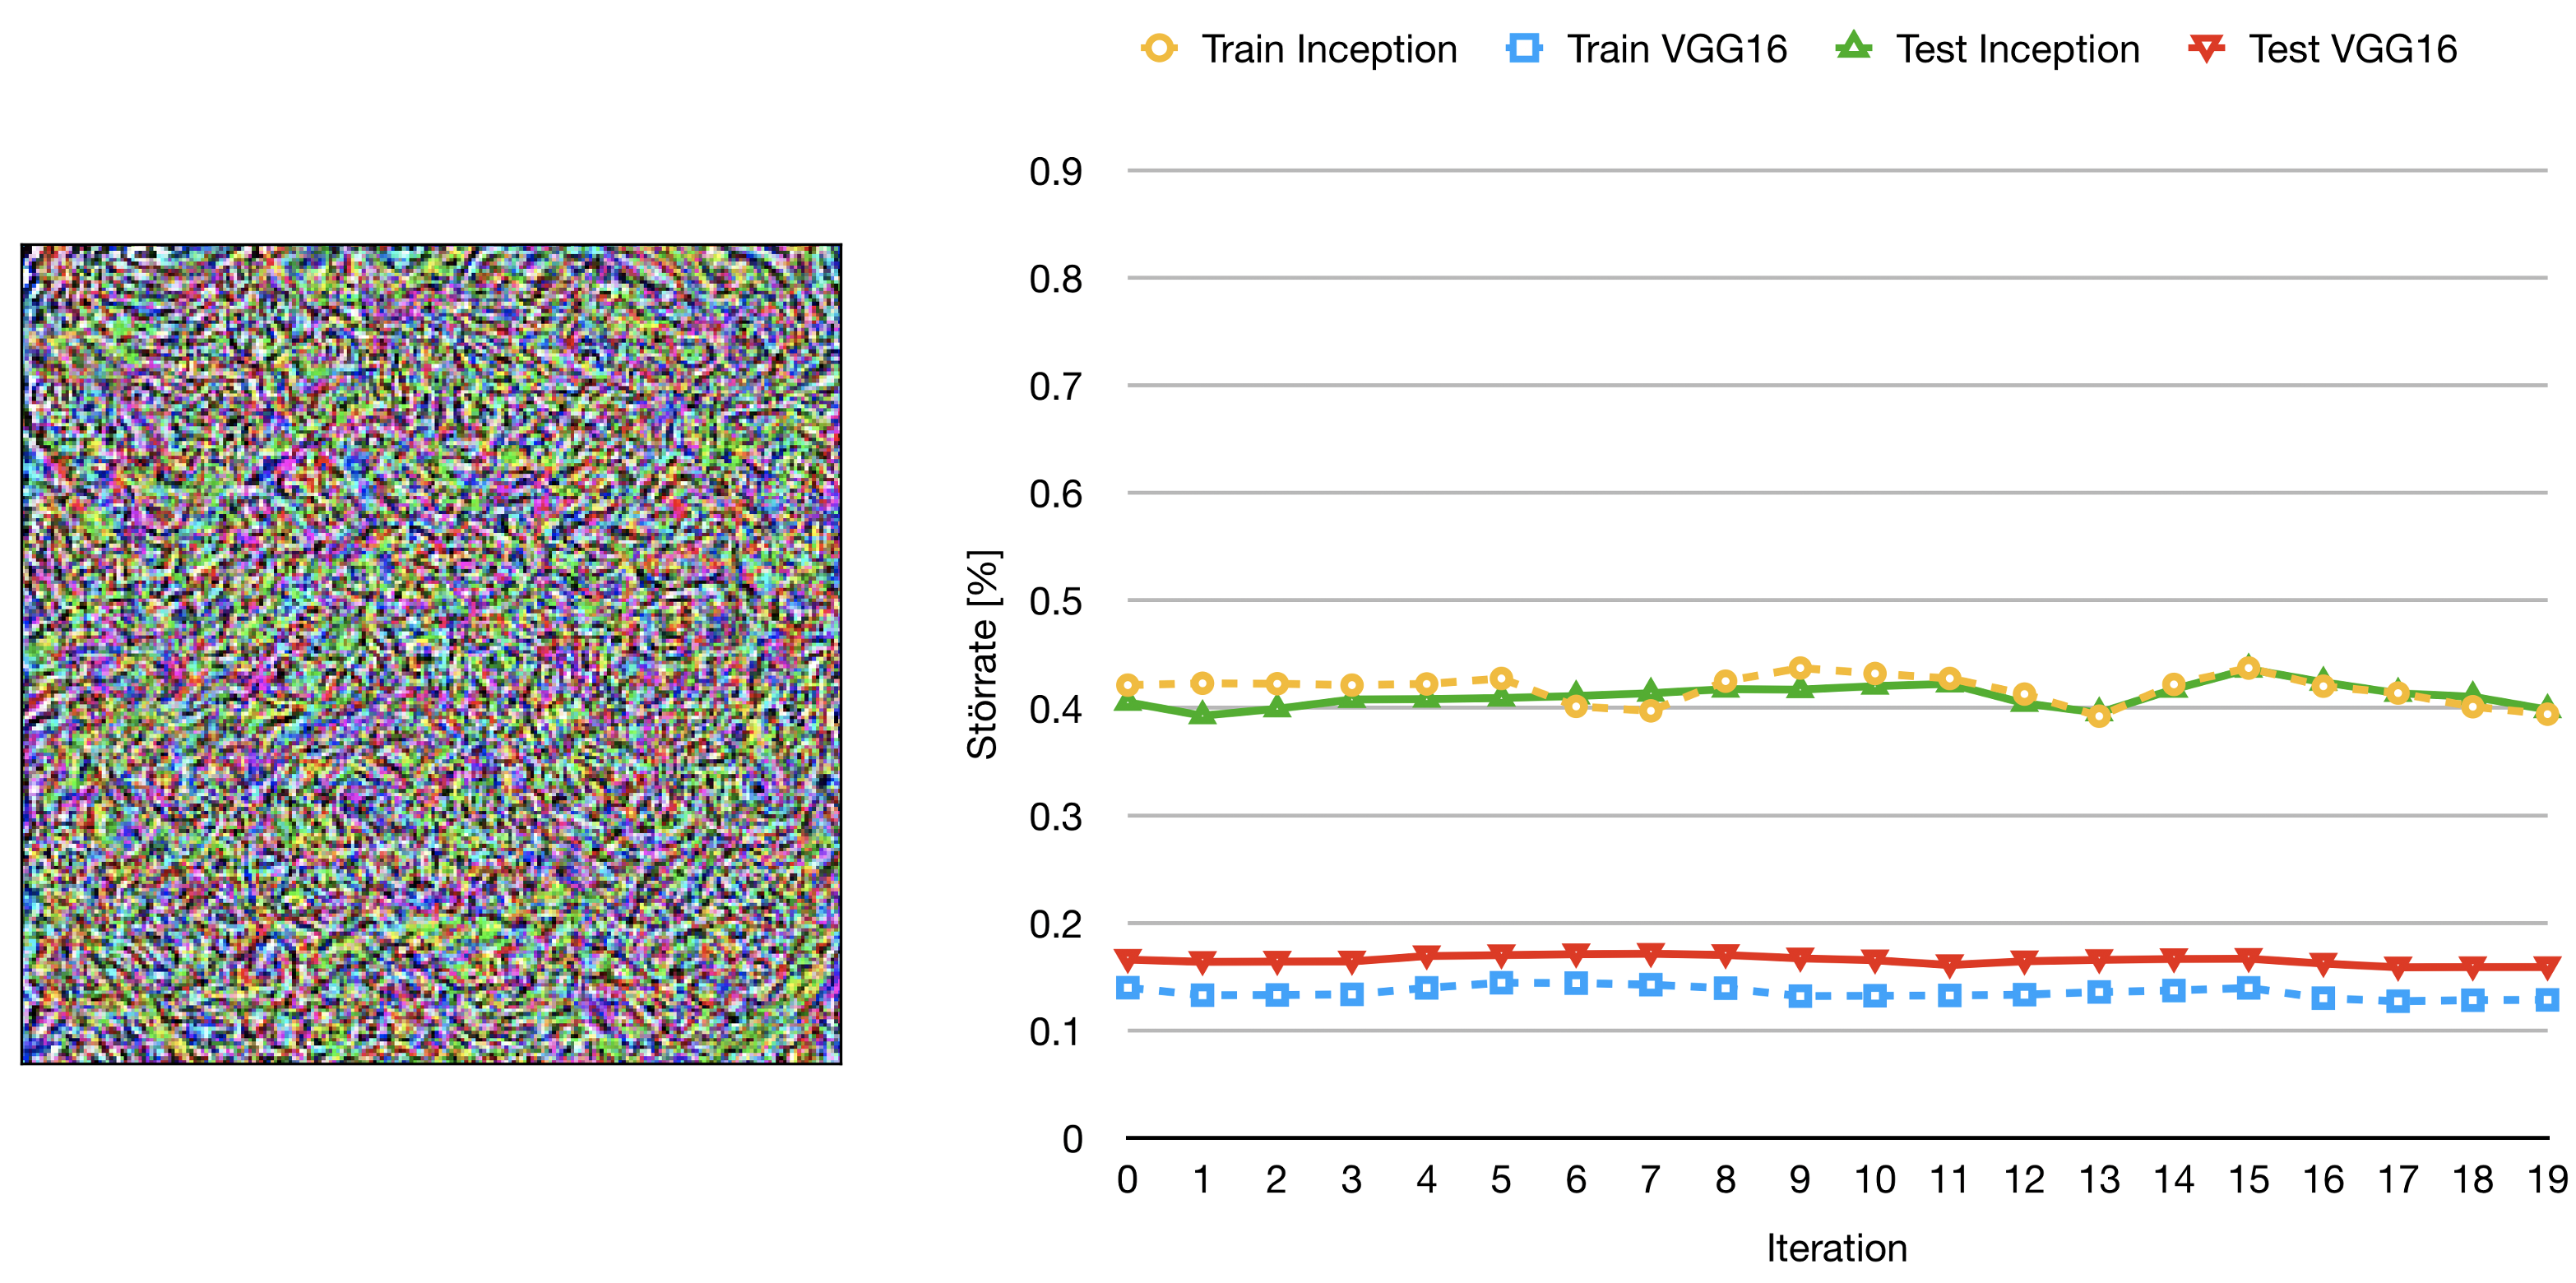
\includegraphics[width=\textwidth]{./images/stoerrate_multifool}
\label{fig_stoerwerte_multifool}
\end{figure}

\section{Vergleich}

In Tabelle \ref{tbl_vergleich_comb} sind die besten erreichten Störraten für Inception, VGG-16 und ResNet-152 auf dem Validation-Set mit den verschiedenen Kombinationsverfahren angegeben. 

Keiner der per linearer Interpolation oder modifiziertem DeepFool erstellten Störwerte konnte die verwendeten Modelle besser stören, als die direkt auf diesen Modellen berechneten Störwerte. Auch auf einem dritten Modell sind die beiden Kombinationen nicht besser.
Der per Finetuning optimierte Störwert erzielt ähnliche Störraten, wie ein rein auf VGG-16 berechneten Störwert. 
Die Störrate auf ResNet-152 beträgt $38.6\%$, was einer absoluten Veränderung von $0.6\%$ entspricht. Auf VGG-16 verschlechterte sich die Störrate wiederum um $0.8\%$.

Der durch abwechselndes Generieren entstandene Störwert erreicht über alle drei Modelle hinweg die höchsten Störraten. 
Er erreicht auf VGG-16 eine höhere Störrate ($60.6\%$), als durch reines Training auf diesem Modell erreicht wurde. 
Zudem wird auf ResNet-152 eine Störrate von $41.2\%$ erreicht. 
Ein nur auf VGG-16 generierter Störwert erreicht $38\%$, die Störrate stieg um $3.2\%$.

\begin{table}[]
\centering
\caption{Vergleich der Störraten von einzelnen Störwerten und Kombinationsverfahren (Validation-Set, $l_\infty$, $\xi=10$). Es werden die besten gemessenen Ergebnisse aufgelistet.}
\begin{tabular}{|l|l|l|l|l|l|}
\hline

											&	Inception	&	VGG-16		&	ResNet-152		\\ \hline
Inception-Störwert							&	$81.9\%$		&	$15.9\%$	&	$15.9\%$		\\
VGG-16-Störwert								&	$59.9\%$		&	$58.7\%$	&	$38.0\%$		\\
ResNet-152-Störwert							&	$54.6\%$		&	$31.4\%$	&	$73.4\%$		\\ \hline
lin. Interpolation ($45\% \overline{PQ}$)	&	$46.2\%$		&	$23.7\%$	&	$16.7\%$		\\
Finetuning									&	$59.9\%$		&	$57.9\%$	&	$38.6\%$		\\
abwechselndes Generieren						&	$67.3\%$		&	$60.6\%$	&	$41.2\%$		\\
modifiziertes DeepFool						&	$43.6\%$		&	$18.4\%$	&	$14.1\%$		\\


\hline 
\end{tabular}
\label{tbl_vergleich_comb}
\end{table}


    
\chapter{Diskussion}

Die Resultate der Reproduktion zeigen, dass mit den UAP- und DeepFool-Verfahren hohe Störraten auf verschiedenen Modellen erreicht werden können. Die erste Forschungsfrage kann aber nicht eindeutig bejaht werden. Für die VGG-16 und VGG-19 Modelle konnten die von Moosavi-Dezfooli et al. in \cite{moosavi-dezfooli_universal_2017-1} gemessenen Störraten nicht erreicht werden. Dafür könnten u.a. die verwendeten Trainingsdaten, die gewählten Parameter oder andere Implementationsdetails verantwortlich sein. In \cite{moosavi-dezfooli_universal_2017-1} wurden einige verwendete Parameter nicht dokumentiert. Diese Arbeit dokumentiert den Einfluss dieser Parameter für weitere Arbeiten mit UAP und DeepFool. Aufgrund fehlender Ressourcen konnten nicht alle Parameter abschliessend getestet werden. Insbesondere die Anzahl getesteter Klassen konnte deshalb nicht ausführlich untersucht werden. Es wäre deshalb naheliegend, dass die bei VGG-16 und VGG-19 gemessenen Differenzen aufgrund dieses Parameters zustande kamen.

Um die zweite Frage zu klären, wurden vier Varianten zur Kombination von Störwerten und Modellen implementiert. Damit soll die Transferierbarkeit der generierten Störwerte erhöht werden. Durch abwechselndes Generieren auf zwei Modellen konnten Störwerte generiert werden, die auf beiden Modellen hohe Störraten erreichen. Auf einem dritten Modell konnten damit nur gering bessere Störraten erreicht werden. Die anderen Kombinationsverfahren lieferten keine besseren Ergebnisse als auf einzelnen Modellen trainierte Störwerte. Insbesondere das Finetuning und die lineare Interpolation können als Kombinationsvarianten ausgeschlossen werden. Das erweiterte DeepFool-Verfahren erzeugte ebenfalls keine besseren Störwerte. Dessen Ergebnisse könnten evtl. durch Wahl von Klassengrenzen mit ähnlicher Richtung verbessert werden. Diese Tests wären notwendig, um die zweite Forschungsfrage abschliessend zu beantworten.

Die Störraten in dieser Thesis waren zwar in einigen Fällen tiefer als in der Originalarbeit, es konnten aber dennoch hohe Störraten und transferierbare Störwerte generiert werden. Das zeigt, dass die Modelle sehr anfällig sind auf Angriffe. Es braucht Schutzmassnahmen vor solchen Angriffen, bevor diese Modelle in kritischen oder potentiell gefährlichen Situationen eingesetzt werden können.


\section{Ausblick}

Aufgrund der begrenzten Ressourcen für diese Arbeit konnten einige Tests nicht durchgeführt werden. Um die erste Forschungsfrage abschliessend zu klären, muss der Einfluss der Anzahl getesteter Klassen mit besserer Hardware weiter untersucht werden. Bei den Tests in dieser Arbeit wurden maximal $200$ der $1'000$ Klassen des Datensatzes in DeepFool beachtet. Diese grosse Anzahl nicht untersuchter Klassen könnte die Unterschiede der Störraten für einige Modelle erklären. 

Hinsichtlich der Kombinationsverfahren gibt es ebenfalls noch zu untersuchende Punkte. Das angepasste DeepFool-Verfahren sucht die Klassengrenzen-Kombination mit minimaler Distanz zum Ausgangsbild. Stattdessen könnte auch ein Klassenpaar mit ähnlicher Richtung (und minimaler Distanz) gewählt werden. Das angepasste Verfahren in dieser Arbeit beachtet die Richtung nicht. Aus zeitlichen Gründen konnte nicht mehr getestet werden, ob dadurch bessere Störwerte entstehen.


\listoffigures

\listoftables

\bibliography{Bachelor-Thesis.bib}
\bibliographystyle{ieeetr}


\newpage

\begin{appendix}


\chapter*{Selbstständigkeitserklärung}
Ich erkläre hiermit, dass ich diese Thesis selbständig verfasst 
und keine andern als die angegebenen Quellen benutzt habe. 
Alle Stellen, die wörtlich oder sinngemäss aus Quellen entnommen wurden, 
habe ich als solche kenntlich gemacht. Ich versichere zudem, dass ich bisher 
noch keine wissenschaftliche Arbeit mit gleichem oder ähnlichem Inhalt an der 
Fernfachhochschule Schweiz oder an einer anderen Hochschule eingereicht habe. 
Mir ist bekannt, dass andernfalls die Fernfachhochschule Schweiz zum Entzug 
des aufgrund dieser Thesis verliehenen Titels berechtigt ist.

\vspace{4cm}
\noindent
\hrule \ \\[-0.5ex]
Ort, Datum, Unterschrift
\end{appendix}


\end{document}


